%%% Notice: This file contains a large number of \verb's 
%DIF LATEXDIFF DIFFERENCE FILE
%DIF DEL PASJ_Takahashi_et_al_2020.tex       Fri Jul 17 19:18:24 2020
%DIF ADD PASJ_Takahashi_et_al_2020_new.tex   Wed Jul 22 16:38:46 2020
%%%         or verbatim environments in order to display command names
%%%         or examples.  But the use of \verb/verbatim is *not* recommended. 
%%% ver.6 2015/01/05 
\documentclass[proof]{pasj01}
\let\square\relax
\usepackage{amsfonts}
\usepackage{graphicx}

%
%\draft 
\Received{$\langle$reception date$\rangle$}
\Accepted{$\langle$acception date$\rangle$}
\Published{$\langle$publication date$\rangle$}
%DIF PREAMBLE EXTENSION ADDED BY LATEXDIFF
%DIF CFONT PREAMBLE %DIF PREAMBLE
\RequirePackage{color}\definecolor{RED}{rgb}{1,0,0}\definecolor{BLUE}{rgb}{0,0,1} %DIF PREAMBLE
\providecommand{\DIFadd}[1]{{\protect\color{blue} \sf #1}} %DIF PREAMBLE
\providecommand{\DIFdel}[1]{{\protect\color{red} \scriptsize #1}} %DIF PREAMBLE
%DIF COLOR PREAMBLE %DIF PREAMBLE
\RequirePackage{color} %DIF PREAMBLE
\providecommand{\DIFaddbegin}{\protect\color{blue}} %DIF PREAMBLE
\providecommand{\DIFaddend}{\protect\color{black}} %DIF PREAMBLE
\providecommand{\DIFdelbegin}{\protect\color{red}} %DIF PREAMBLE
\providecommand{\DIFdelend}{\protect\color{black}} %DIF PREAMBLE
%DIF FLOATSAFE PREAMBLE %DIF PREAMBLE
\providecommand{\DIFaddFL}[1]{\DIFadd{#1}} %DIF PREAMBLE
\providecommand{\DIFdelFL}[1]{\DIFdel{#1}} %DIF PREAMBLE
\providecommand{\DIFaddbeginFL}{} %DIF PREAMBLE
\providecommand{\DIFaddendFL}{} %DIF PREAMBLE
\providecommand{\DIFdelbeginFL}{} %DIF PREAMBLE
\providecommand{\DIFdelendFL}{} %DIF PREAMBLE
\newcommand{\DIFscaledelfig}{0.5}
%DIF HIGHLIGHTGRAPHICS PREAMBLE %DIF PREAMBLE
\RequirePackage{settobox} %DIF PREAMBLE
\RequirePackage{letltxmacro} %DIF PREAMBLE
\newsavebox{\DIFdelgraphicsbox} %DIF PREAMBLE
\newlength{\DIFdelgraphicswidth} %DIF PREAMBLE
\newlength{\DIFdelgraphicsheight} %DIF PREAMBLE
% store original definition of \includegraphics %DIF PREAMBLE
\LetLtxMacro{\DIFOincludegraphics}{\includegraphics} %DIF PREAMBLE
\newcommand{\DIFaddincludegraphics}[2][]{{\color{blue}\fbox{\DIFOincludegraphics[#1]{#2}}}} %DIF PREAMBLE
\newcommand{\DIFdelincludegraphics}[2][]{% %DIF PREAMBLE
\sbox{\DIFdelgraphicsbox}{\DIFOincludegraphics[#1]{#2}}% %DIF PREAMBLE
\settoboxwidth{\DIFdelgraphicswidth}{\DIFdelgraphicsbox} %DIF PREAMBLE
\settoboxtotalheight{\DIFdelgraphicsheight}{\DIFdelgraphicsbox} %DIF PREAMBLE
\scalebox{\DIFscaledelfig}{% %DIF PREAMBLE
\parbox[b]{\DIFdelgraphicswidth}{\usebox{\DIFdelgraphicsbox}\\[-\baselineskip] \rule{\DIFdelgraphicswidth}{0em}}\llap{\resizebox{\DIFdelgraphicswidth}{\DIFdelgraphicsheight}{% %DIF PREAMBLE
\setlength{\unitlength}{\DIFdelgraphicswidth}% %DIF PREAMBLE
\begin{picture}(1,1)% %DIF PREAMBLE
\thicklines\linethickness{2pt} %DIF PREAMBLE
{\color[rgb]{1,0,0}\put(0,0){\framebox(1,1){}}}% %DIF PREAMBLE
{\color[rgb]{1,0,0}\put(0,0){\line( 1,1){1}}}% %DIF PREAMBLE
{\color[rgb]{1,0,0}\put(0,1){\line(1,-1){1}}}% %DIF PREAMBLE
\end{picture}% %DIF PREAMBLE
}\hspace*{3pt}}} %DIF PREAMBLE
} %DIF PREAMBLE
\LetLtxMacro{\DIFOaddbegin}{\DIFaddbegin} %DIF PREAMBLE
\LetLtxMacro{\DIFOaddend}{\DIFaddend} %DIF PREAMBLE
\LetLtxMacro{\DIFOdelbegin}{\DIFdelbegin} %DIF PREAMBLE
\LetLtxMacro{\DIFOdelend}{\DIFdelend} %DIF PREAMBLE
\DeclareRobustCommand{\DIFaddbegin}{\DIFOaddbegin \let\includegraphics\DIFaddincludegraphics} %DIF PREAMBLE
\DeclareRobustCommand{\DIFaddend}{\DIFOaddend \let\includegraphics\DIFOincludegraphics} %DIF PREAMBLE
\DeclareRobustCommand{\DIFdelbegin}{\DIFOdelbegin \let\includegraphics\DIFdelincludegraphics} %DIF PREAMBLE
\DeclareRobustCommand{\DIFdelend}{\DIFOaddend \let\includegraphics\DIFOincludegraphics} %DIF PREAMBLE
\LetLtxMacro{\DIFOaddbeginFL}{\DIFaddbeginFL} %DIF PREAMBLE
\LetLtxMacro{\DIFOaddendFL}{\DIFaddendFL} %DIF PREAMBLE
\LetLtxMacro{\DIFOdelbeginFL}{\DIFdelbeginFL} %DIF PREAMBLE
\LetLtxMacro{\DIFOdelendFL}{\DIFdelendFL} %DIF PREAMBLE
\DeclareRobustCommand{\DIFaddbeginFL}{\DIFOaddbeginFL \let\includegraphics\DIFaddincludegraphics} %DIF PREAMBLE
\DeclareRobustCommand{\DIFaddendFL}{\DIFOaddendFL \let\includegraphics\DIFOincludegraphics} %DIF PREAMBLE
\DeclareRobustCommand{\DIFdelbeginFL}{\DIFOdelbeginFL \let\includegraphics\DIFdelincludegraphics} %DIF PREAMBLE
\DeclareRobustCommand{\DIFdelendFL}{\DIFOaddendFL \let\includegraphics\DIFOincludegraphics} %DIF PREAMBLE
%DIF END PREAMBLE EXTENSION ADDED BY LATEXDIFF

\begin{document}

\title{Photometric classification of \DIFdelbegin \DIFdel{the }\DIFdelend HSC transients \DIFdelbegin \DIFdel{through }\DIFdelend \DIFaddbegin \DIFadd{using }\DIFaddend machine learning}
\author{
Ichiro \textsc{Takahashi}\altaffilmark{1,2,4,*},
Nao \textsc{Suzuki}\altaffilmark{1},
Naoki \textsc{Yasuda}\altaffilmark{1},
Akisato \textsc{Kimura}\altaffilmark{3},
Naonori \textsc{Ueda}\altaffilmark{3},
Masaomi \textsc{Tanaka}\altaffilmark{4,1},
Nozomu \textsc{Tominaga}\altaffilmark{5,1},
and
Naoki \textsc{Yoshida}\altaffilmark{1,2,6,7}
%
}%
\altaffiltext{1}{Kavli Institute for the Physics and Mathematics of the Universe (WPI), The University of Tokyo Institutes for Advanced Study, The University of Tokyo, 5-1-5 Kashiwanoha, Kashiwa, Chiba 277-8583, Japan}
\altaffiltext{2}{CREST, JST, 4-1-8 Honcho, Kawaguchi, Saitama 332-0012, Japan}
\altaffiltext{3}{NTT Communication Science Laboratories, 2-4 Hikaridai, Seika-cho, Keihanna Science City, Kyoto 619-0237, Japan}
\altaffiltext{4}{Astronomical Institute, Tohoku University, Aoba, Sendai, Miyagi 980-8578, Japan}
\altaffiltext{5}{Department of Physics, Faculty of Science and Engineering, Konan University, 8-9-1 Okamoto, Kobe, Hyogo 658-8501, Japan}
\altaffiltext{6}{Department of Physics, Graduate School of Science, The University of Tokyo, 7-3-1 Hongo, Bunkyo-ku, Tokyo 113-0033, Japan}
\altaffiltext{7}{Institute for Physics of Intelligence, The University of Tokyo, 7-3-1 Hongo, Bunkyo-ku, Tokyo 113-0033, Japan}

\email{ichiro.takahashi@ipmu.jp}

\KeyWords{supernovae: general --- methods: statistical --- surveys}

\maketitle
%
\begin{abstract}
The advancement of technology has \DIFdelbegin \DIFdel{brought }\DIFdelend \DIFaddbegin \DIFadd{resulted in }\DIFaddend a rapid increase \DIFdelbegin \DIFdel{of }\DIFdelend \DIFaddbegin \DIFadd{in }\DIFaddend supernova discoveries. \DIFaddbegin \DIFadd{The }\DIFaddend Subaru Hyper Suprime-Cam (HSC) Transient \DIFdelbegin \DIFdel{survey}\DIFdelend \DIFaddbegin \DIFadd{Survey}\DIFaddend , conducted from \DIFdelbegin \DIFdel{Fall }\DIFdelend \DIFaddbegin \DIFadd{fall }\DIFaddend 2016 through \DIFdelbegin \DIFdel{Spring }\DIFdelend \DIFaddbegin \DIFadd{spring }\DIFaddend 2017, yielded 1824 supernova candidates. \DIFdelbegin \DIFdel{We are in need of }\DIFdelend \DIFaddbegin \DIFadd{This gave rise to the need for }\DIFaddend fast type classification for spectroscopic follow-up and \DIFdelbegin \DIFdel{developed a machine learning algorithm using Deep Neural Network }\DIFdelend \DIFaddbegin \DIFadd{prompted us to develop a machine-learning algorithm using a deep neural network }\DIFaddend (DNN) with \DIFdelbegin \DIFdel{Highway }\DIFdelend \DIFaddbegin \DIFadd{highway }\DIFaddend layers. 
This machine is trained by actual observed cadence and filter combinations \DIFdelbegin \DIFdel{so }\DIFdelend \DIFaddbegin \DIFadd{such }\DIFaddend that we can directly input \DIFaddbegin \DIFadd{the }\DIFaddend observed data array into \DIFaddbegin \DIFadd{the }\DIFaddend machine without any interpretation. We \DIFdelbegin \DIFdel{test }\DIFdelend \DIFaddbegin \DIFadd{tested }\DIFaddend our model with a \DIFdelbegin \DIFdel{data set from }\DIFdelend \DIFaddbegin \DIFadd{dataset from the }\DIFaddend LSST classification challenge (Deep Drilling Field only).
Our classifier scores \DIFaddbegin \DIFadd{an }\DIFaddend AUC of 0.996 for binary classification (SN~Ia or non-Ia) and 95.3\% \DIFdelbegin \DIFdel{in }\DIFdelend accuracy for three-class classification (SN~Ia, SN~Ibc\DIFdelbegin \DIFdel{and }\DIFdelend \DIFaddbegin \DIFadd{, or }\DIFaddend SN~II). \DIFdelbegin \DIFdel{When we apply }\DIFdelend \DIFaddbegin \DIFadd{Application of }\DIFaddend our binary classification to HSC \DIFdelbegin \DIFdel{Transient data , AUC score becomes }\DIFdelend \DIFaddbegin \DIFadd{transient data yields an AUC score of }\DIFaddend 0.925. With two weeks of HSC data since the first detection, this classifier achieves 78.1\% \DIFdelbegin \DIFdel{in }\DIFdelend accuracy for binary classification, and \DIFdelbegin \DIFdel{it }\DIFdelend \DIFaddbegin \DIFadd{the accuracy }\DIFaddend increases to 84.2\% with \DIFdelbegin \DIFdel{full data set. The }\DIFdelend \DIFaddbegin \DIFadd{the full dataset. This paper discusses the }\DIFaddend potential use of machine learning \DIFdelbegin \DIFdel{is being discussed}\DIFdelend \DIFaddbegin \DIFadd{for supernova type classification purposes}\DIFaddend .
\end{abstract}

\section{Introduction}
Time domain science \DIFdelbegin \DIFdel{becomes one of the major fields }\DIFdelend \DIFaddbegin \DIFadd{has become a major field }\DIFaddend of astronomical study\DIFdelbegin \DIFdel{today}\DIFdelend . The discovery of \DIFaddbegin \DIFadd{the }\DIFaddend accelerating universe \citep{perlmutter99a,riess98a} evoked a series of large supernova (SN) surveys in the last \DIFaddbegin \DIFadd{few }\DIFaddend decades 
\citep{betoule14a,scolnic18a,brout19a}.  
These surveys revealed that \DIFdelbegin \DIFdel{there exist a whole }\DIFdelend \DIFaddbegin \DIFadd{an entirely }\DIFaddend new family of transients \DIFaddbegin \DIFadd{exists }\DIFaddend and the search for unknown populations is \DIFaddbegin \DIFadd{currently }\DIFaddend of great interest \DIFdelbegin \DIFdel{today }\DIFdelend \citep{howell06a,phillips07a,quimby07b}. 
For \DIFdelbegin \DIFdel{the }\DIFdelend precision cosmology, it is \DIFdelbegin \DIFdel{very important to keep }\DIFdelend \DIFaddbegin \DIFadd{highly important to maintain }\DIFaddend the purity of \DIFaddbegin \DIFadd{a }\DIFaddend Type Ia supernova (SN~Ia) while \DIFdelbegin \DIFdel{having uniform sampling }\DIFdelend \DIFaddbegin \DIFadd{performing uniform sampling of these supernovae (SNe~Ia) ranging }\DIFaddend from bright to faint\DIFdelbegin \DIFdel{SNe~Ia}\DIFdelend . Spectroscopic follow-up has been essential to distinguish \DIFaddbegin \DIFadd{a }\DIFaddend faint SN~Ia from \DIFaddbegin \DIFadd{a }\DIFaddend Type Ib supernova (SN~Ib) and \DIFaddbegin \DIFadd{a }\DIFaddend Type Ic supernova (SN~Ic)\DIFaddbegin \DIFadd{, }\DIFaddend which have similar light curve behavior \citep{scolnic14a}. \DIFdelbegin \DIFdel{A }\DIFdelend \DIFaddbegin \DIFadd{Considering that a }\DIFaddend large amount of precious telescope time is dedicated to \DIFdelbegin \DIFdel{the }\DIFdelend \DIFaddbegin \DIFadd{these }\DIFaddend follow-up programs, \DIFdelbegin \DIFdel{and we would like to make an }\DIFdelend \DIFaddbegin \DIFadd{it is desirable to make }\DIFaddend efficient use of \DIFdelbegin \DIFdel{those }\DIFdelend \DIFaddbegin \DIFadd{these }\DIFaddend telescopes.

The scale of \DIFdelbegin \DIFdel{survey is getting }\DIFdelend \DIFaddbegin \DIFadd{surveys is becoming }\DIFaddend larger, and it \DIFdelbegin \DIFdel{becomes }\DIFdelend \DIFaddbegin \DIFadd{has become }\DIFaddend impossible to trigger spectroscopic follow-up for all of the candidates in real time\DIFdelbegin \DIFdel{, and we are in need of developing }\DIFdelend \DIFaddbegin \DIFadd{. It has therefore become necessary to develop a }\DIFaddend new classification scheme\DIFdelbegin \DIFdel{.  It is }\DIFdelend \DIFaddbegin \DIFadd{, and }\DIFaddend a natural path \DIFdelbegin \DIFdel{to }\DIFdelend \DIFaddbegin \DIFadd{along which to proceed would be to }\DIFaddend perform photometric classification \citep{sako11a,jonesl8a}. \DIFdelbegin \DIFdel{With the rise of Machine Learning Technologies, it is getting common that an }\DIFdelend \DIFaddbegin \DIFadd{The rise of machine-learning technologies has resulted in }\DIFaddend astronomical big data \DIFdelbegin \DIFdel{is being analyzed through machine learning}\DIFdelend \DIFaddbegin \DIFadd{commonly being analyzed by using machine-learning techniques}\DIFaddend .   

Neural \DIFdelbegin \DIFdel{Network has }\DIFdelend \DIFaddbegin \DIFadd{networks have }\DIFaddend been used for photometric redshift studies from the early \DIFdelbegin \DIFdel{stage.  Today, many Machine Learning methods are applied to the photometric redshift studies }\DIFdelend \DIFaddbegin \DIFadd{stages and these studies often involve the use of machine-learning methods }\DIFaddend \citep{collister04a,carliles10a,pasquet19a}.
Deep \DIFdelbegin \DIFdel{Neural Network (DNN) is now being used for imaging data for finding strong lens system }\DIFdelend \DIFaddbegin \DIFadd{neural networks (DNNs) are being used to process imaging data to identify strong lens systems }\DIFaddend \citep{petrillo17a} or for galaxy morphology classifications \citep{hausen19a}. \DIFdelbegin \DIFdel{Now}\DIFdelend \DIFaddbegin \DIFadd{Currently}\DIFaddend , machine learning is being introduced \DIFdelbegin \DIFdel{for transient survey }\DIFdelend \DIFaddbegin \DIFadd{to process transient survey data }\DIFaddend for detection \citep{goldstein15a} and classification \DIFaddbegin \DIFadd{purposes }\DIFaddend \citep{charnock17a}.

In this paper, we introduce our attempt to apply machine learning (DNN) to \DIFdelbegin \DIFdel{the }\DIFdelend actual transient survey data.
\DIFaddbegin \DIFadd{The }\DIFaddend Hyper Suprime-Cam (HSC) \citep{miyazaki18a,Komiyama2018,kawanomoto18a,Furusawa2018}\DIFdelbegin \DIFdel{on Subaru Telescope enables us to probe }\DIFdelend \DIFaddbegin \DIFadd{, a gigantic mosaic CCD still camera mounted on the 8.2 m Subaru Telescope, makes it possible to probe a }\DIFaddend wide field (1.77 deg$^2$ \DIFdelbegin \DIFdel{Field of View}\DIFdelend \DIFaddbegin \DIFadd{field of view}\DIFaddend ) and deep space (26th mag in \DIFaddbegin \DIFadd{the }\DIFaddend $i-$band / epoch). Our primary scientific goals are SN~Ia cosmology, Type II supernova (SN~II) cosmology, \DIFaddbegin \DIFadd{and }\DIFaddend super-luminous supernova (SLSN) studies as well as \DIFdelbegin \DIFdel{probing unknown population }\DIFdelend \DIFaddbegin \DIFadd{to probe unknown populations }\DIFaddend of transients.  
As \DIFdelbegin \DIFdel{is reported in }\DIFdelend \DIFaddbegin \DIFadd{reported recently }\DIFaddend \citet{yasuda19a}, more than 1800 SNe \DIFdelbegin \DIFdel{are discovered in }\DIFdelend \DIFaddbegin \DIFadd{were discovered during }\DIFaddend a 6-month campaign. 
We deployed \DIFdelbegin \DIFdel{a }\DIFdelend machine learning (AUC boosting) for transient detection \citep{morii16a}, where \DIFdelbegin \DIFdel{'real' vs. 'bogus' is determined by a machine.In }\DIFdelend \DIFaddbegin \DIFadd{the machine determines whether a transient is ``real'' or ``bogus.''
Previously }\DIFaddend \citet{Kimura17}, we adopted \DIFaddbegin \DIFadd{a }\DIFaddend DNN for SN type classification from \DIFdelbegin \DIFdel{2 dimensional }\DIFdelend \DIFaddbegin \DIFadd{a two-dimensional }\DIFaddend image, and highway block \DIFdelbegin \DIFdel{is }\DIFdelend \DIFaddbegin \DIFadd{was }\DIFaddend introduced for the optimization of layers.
This \DIFdelbegin \DIFdel{paper }\DIFdelend \DIFaddbegin \DIFadd{research }\DIFaddend is an extension of \DIFaddbegin \DIFadd{our previous work }\DIFaddend \citet{Kimura17} and applies \DIFaddbegin \DIFadd{a }\DIFaddend DNN to the photometric classification of transients.   
\DIFdelbegin \DIFdel{Our unique attempt is to make use of }\DIFdelend \DIFaddbegin \DIFadd{We uniquely attempt to use }\DIFaddend the observed data \DIFdelbegin \DIFdel{as 'raw' as possible so that we can directly plug them into machine without any fitting to }\DIFdelend \DIFaddbegin \DIFadd{in a state that is as ``raw'' as possible to enable us to directly use the data as input for the machine without fitting }\DIFaddend the data or extracting characteristics.

The structure of this paper is as follows. We introduce our methods in section 2, and \DIFaddbegin \DIFadd{the }\DIFaddend data in section 3. The design of our DNN model and its application to pseudo-real LSST simulation data is described in section 4. Section 5 \DIFdelbegin \DIFdel{shows }\DIFdelend \DIFaddbegin \DIFadd{presents }\DIFaddend the application of our model to the actual Subaru/HSC data. We discuss the results in section 6 and \DIFdelbegin \DIFdel{conclusion is given }\DIFdelend \DIFaddbegin \DIFadd{conclude the paper }\DIFaddend in section 7.
%
%

\section{Methods}
\subsection{Tasks in HSC survey}
\label{sec:tasks}
\DIFaddbegin \DIFadd{The }\DIFaddend Subaru HSC Transient \DIFdelbegin \DIFdel{survey is a part of }\DIFdelend \DIFaddbegin \DIFadd{Survey forms part of the }\DIFaddend Subaru Strategic Project (SSP)\DIFaddbegin \DIFadd{, }\DIFaddend which is a five-year program \DIFdelbegin \DIFdel{with }\DIFdelend \DIFaddbegin \DIFadd{that includes a total of }\DIFaddend 300 dark nights \citep{aihara18a,miyazaki18a}.
\DIFaddbegin \DIFadd{The }\DIFaddend HSC-SSP Transient Survey is composed of two seasons, \DIFdelbegin \DIFdel{and the first season is executed for a consecutive 6 }\DIFdelend \DIFaddbegin \DIFadd{the first of which was executed for six consecutive }\DIFaddend months from November 2016 through April 2017.
\DIFaddbegin \DIFadd{The }\DIFaddend HSC is mounted on \DIFdelbegin \DIFdel{the }\DIFdelend prime focus for \DIFdelbegin \DIFdel{2 }\DIFdelend \DIFaddbegin \DIFadd{two }\DIFaddend weeks in dark time.   
Weather permitted, we \DIFdelbegin \DIFdel{aim to observe 2 }\DIFdelend \DIFaddbegin \DIFadd{aimed to observe two }\DIFaddend data points per filter per lunation.
\DIFdelbegin \DIFdel{A detailed }\DIFdelend \DIFaddbegin \DIFadd{Details of the }\DIFaddend survey strategies and the observing logs \DIFdelbegin \DIFdel{are reported in }\DIFdelend \DIFaddbegin \DIFadd{were reported }\DIFaddend \citet{yasuda19a}, and we \DIFdelbegin \DIFdel{use the observed photometric data described in \citet{yasuda19a} }\DIFdelend \DIFaddbegin \DIFadd{used the reported photometric data \citet{yasuda19a} to develop the machine-learning method}\DIFaddend .

One of our primary goals \DIFdelbegin \DIFdel{of }\DIFdelend \DIFaddbegin \DIFadd{with the }\DIFaddend HSC-SSP Transient Survey is SN~Ia Cosmology\DIFaddbegin \DIFadd{, }\DIFaddend which aims to perform the most precise measurement of dark energy at high-redshift and test \DIFdelbegin \DIFdel{if dark energy is changing in time or not }\DIFdelend \DIFaddbegin \DIFadd{whether the dark energy varies with time }\DIFaddend \citep{linder03b}.
We \DIFdelbegin \DIFdel{are }\DIFdelend \DIFaddbegin \DIFadd{have been }\DIFaddend awarded 96 orbits of \DIFdelbegin \DIFdel{the }\DIFdelend Hubble Space Telescope time (WFC3 Camera) to execute \DIFdelbegin \DIFdel{a precise photometry on IR }\DIFdelend \DIFaddbegin \DIFadd{precise IR photometry }\DIFaddend at the time of maximum.
Our HST program uses non-disrupted ToO\DIFaddbegin \DIFadd{, }\DIFaddend which means we \DIFdelbegin \DIFdel{send the observing request }\DIFdelend \DIFaddbegin \DIFadd{are required to send the request for observation latest }\DIFaddend by Wednesday, \DIFdelbegin \DIFdel{2 }\DIFdelend \DIFaddbegin \DIFadd{two }\DIFaddend weeks prior to the observation.
In other words, we \DIFdelbegin \DIFdel{are in need of finding good candidates 2-3 }\DIFdelend \DIFaddbegin \DIFadd{need to identify good candidates 2--3 }\DIFaddend weeks prior to the maximum. \DIFdelbegin \DIFdel{High-redshift }\DIFdelend \DIFaddbegin \DIFadd{Although a high-redshift }\DIFaddend (z$>$1) time dilation factor helps, \DIFdelbegin \DIFdel{but }\DIFdelend it is always a challenge to identify SN~Ia on the rise.

Our international collaboration team executes spectroscopic follow-up using \DIFaddbegin \DIFadd{the }\DIFaddend large telescopes in the world.  
Our target, high-redshift SN~Ia, is faint ($\sim$ 24th mag in \DIFaddbegin \DIFadd{the }\DIFaddend $i-$band) for spectroscopic identification even with the \DIFaddbegin \DIFadd{most }\DIFaddend powerful large telescopes: GMOS Gemini \citep{hook04a}, GTC, Keck LRIS \citep{oke95a}, VLT FORS, Subaru FOCAS \citep{kashikawa02a}\DIFaddbegin \DIFadd{, }\DIFaddend and AAT AAOMega Spectrograph.  
Thus, it is critical to hit the target at the time of maximum \DIFdelbegin \DIFdel{either by }\DIFdelend \DIFaddbegin \DIFadd{brightness either by using }\DIFaddend ToO (GTC), queue mode (VLT)\DIFaddbegin \DIFadd{, }\DIFaddend or classical scheduled observation (Keck, Subaru, ATT).

\DIFdelbegin \DIFdel{For }\DIFdelend \DIFaddbegin \DIFadd{An }\DIFaddend SN~Ia \DIFdelbegin \DIFdel{, it takes about }\DIFdelend \DIFaddbegin \DIFadd{requires approximately }\DIFaddend 18 days from its explosion to \DIFdelbegin \DIFdel{the }\DIFdelend \DIFaddbegin \DIFadd{reach its }\DIFaddend maximum in rest frame \citep{conley06a,papadogiannakis19a}. Given \DIFdelbegin \DIFdel{the fact, we are looking at }\DIFdelend \DIFaddbegin \DIFadd{this fact, the supernovae with which we are concerned is }\DIFaddend high-redshift SN~Ia (z$>$1), \DIFdelbegin \DIFdel{we have about a month in }\DIFdelend \DIFaddbegin \DIFadd{in which case we have approximately one month in the }\DIFaddend observed frame for \DIFdelbegin \DIFdel{a }\DIFdelend \DIFaddbegin \DIFadd{an }\DIFaddend SN~Ia from \DIFdelbegin \DIFdel{explosion to the }\DIFdelend \DIFaddbegin \DIFadd{the time of explosion until it reaches its }\DIFaddend maximum. However, our task is to identify \DIFdelbegin \DIFdel{them 2 }\DIFdelend \DIFaddbegin \DIFadd{these supernovae two }\DIFaddend weeks prior to the maximum, \DIFdelbegin \DIFdel{meaning }\DIFdelend \DIFaddbegin \DIFadd{which means }\DIFaddend we have only 2 data points per \DIFdelbegin \DIFdel{a }\DIFdelend filter. In addition to that, \DIFdelbegin \DIFdel{sky condition keeps changing}\DIFdelend \DIFaddbegin \DIFadd{the sky conditions continue to change}\DIFaddend , and we may not have the data as \DIFdelbegin \DIFdel{we originally had }\DIFdelend \DIFaddbegin \DIFadd{originally }\DIFaddend planned. In reality, our identification has to \DIFdelbegin \DIFdel{be done through missing data points }\DIFdelend \DIFaddbegin \DIFadd{proceed despite data points being missing }\DIFaddend on the rise.

In parallel to \DIFaddbegin \DIFadd{the }\DIFaddend SN~Ia Cosmology program, our sister projects also \DIFdelbegin \DIFdel{needs }\DIFdelend \DIFaddbegin \DIFadd{need }\DIFaddend identification and classification of HSC \DIFdelbegin \DIFdel{transient.   
}\DIFdelend \DIFaddbegin \DIFadd{transients.   
Specifically, the }\DIFaddend SN~II cosmology program \DIFdelbegin \DIFdel{needs a }\DIFdelend \DIFaddbegin \DIFadd{requires }\DIFaddend timely spectroscopic follow-up to measure the \DIFdelbegin \DIFdel{expansion velocity of photosphere from }\DIFdelend \DIFaddbegin \DIFadd{velocity at which the photosphere is expanding from the }\DIFaddend H$\beta$ line \citep{dejaeger17a}.
\DIFaddbegin \DIFadd{An }\DIFaddend SLSN is of great interest today, \DIFdelbegin \DIFdel{it is relatively a }\DIFdelend \DIFaddbegin \DIFadd{because it is a relatively }\DIFaddend rare event\citep{quimby11a}\DIFdelbegin \DIFdel{and its mechanism has quite a diversity }\DIFdelend \DIFaddbegin \DIFadd{. SLSN occur via quite a diverse range of mechanisms }\DIFaddend \citep{galyam12a,Moriya18SLSN}, and \DIFdelbegin \DIFdel{it can probe high redshift }\DIFdelend \DIFaddbegin \DIFadd{can be used to probe the high-redshift }\DIFaddend universe \citep{cooke12a}.    
For \DIFaddbegin \DIFadd{the }\DIFaddend SLSN project, timely spectroscopic follow-up is also critical \citep{moriya19a,curtin19a}.

\DIFdelbegin \DIFdel{Early }\DIFdelend \DIFaddbegin \DIFadd{An early }\DIFaddend phase SN~Ia \DIFdelbegin \DIFdel{gives us clues on }\DIFdelend \DIFaddbegin \DIFadd{provides us with clues on the }\DIFaddend explosion mechanism \citep{maeda18a} and progenitors \citep{cao15a}, and it is a \DIFdelbegin \DIFdel{hot }\DIFdelend \DIFaddbegin \DIFadd{popular }\DIFaddend topic to study.
\DIFdelbegin \DIFdel{HSC has an advantage of surveying }\DIFdelend \DIFaddbegin \DIFadd{The advantage of HSC is its ability to survey }\DIFaddend a large volume\DIFdelbegin \DIFdel{and has revealed long standing theory prediction of Helium-shell }\DIFdelend \DIFaddbegin \DIFadd{, and in practice, it has confirmed the long-standing theoretical prediction of helium-shell }\DIFaddend detonation \citep{Jiang2017}.
\DIFdelbegin \DIFdel{Finding }\DIFdelend \DIFaddbegin \DIFadd{Identifying an }\DIFaddend early phase SN~Ia is not \DIFdelbegin \DIFdel{trivial but HSC is }\DIFdelend \DIFaddbegin \DIFadd{a trivial matter but HSC has been }\DIFaddend yielding a new set of early phase SN~Ia \DIFaddbegin \DIFadd{discoveries }\DIFaddend \citep{Jiang_2020}.
Observations of \DIFdelbegin \DIFdel{the }\DIFdelend early phase Core-Collapse \DIFdelbegin \DIFdel{SN provides us with a }\DIFdelend \DIFaddbegin \DIFadd{SNe provide us with }\DIFaddend crucial information on the size of the progenitors \citep{thompson03a,tominaga11a} and Circumstellar Medium \citep{forster18a}.  


\subsection{Classification method for HSC-SSP \DIFdelbegin \DIFdel{transient survey}\DIFdelend \DIFaddbegin \DIFadd{Transient Survey}\DIFaddend }
We designed two \DIFdelbegin \DIFdel{models of machine learning with }\DIFdelend \DIFaddbegin \DIFadd{machine-learning models with the }\DIFaddend emphasis on identifying SN~Ia\DIFdelbegin \DIFdel{which requires time sensitive }\DIFdelend \DIFaddbegin \DIFadd{, which requires a time-sensitive }\DIFaddend trigger for HST IR follow-up.
\DIFdelbegin \DIFdel{One model is in a }\DIFdelend \DIFaddbegin \DIFadd{The first model operates in }\DIFaddend binary mode and classifies \DIFdelbegin \DIFdel{if }\DIFdelend \DIFaddbegin \DIFadd{whether }\DIFaddend a transient is \DIFaddbegin \DIFadd{of the }\DIFaddend SN~Ia \DIFdelbegin \DIFdel{or not.
It has been known that }\DIFdelend \DIFaddbegin \DIFadd{type.
In this regard, }\DIFaddend the majority of high-redshift transients are \DIFaddbegin \DIFadd{known to be of the }\DIFaddend SN~Ia \DIFdelbegin \DIFdel{, and we seek }\DIFdelend \DIFaddbegin \DIFadd{type, and our work entails searching }\DIFaddend for other unknown transients from \DIFdelbegin \DIFdel{the ones labeled as }\DIFdelend \DIFaddbegin \DIFadd{among those labeled }\DIFaddend non-SN~Ia.   
The \DIFdelbegin \DIFdel{other }\DIFdelend \DIFaddbegin \DIFadd{second }\DIFaddend model classifies a transient into \DIFdelbegin \DIFdel{3 }\DIFdelend \DIFaddbegin \DIFadd{one of three }\DIFaddend classes: SN~Ia, SN~Ibc\DIFdelbegin \DIFdel{and }\DIFdelend \DIFaddbegin \DIFadd{, or }\DIFaddend SN~II.  
\DIFdelbegin \DIFdel{We choose three classes }\DIFdelend \DIFaddbegin \DIFadd{These three classes were chosen }\DIFaddend for simplicity and in fact, the majority of SNe \DIFdelbegin \DIFdel{goes }\DIFdelend \DIFaddbegin \DIFadd{belong }\DIFaddend to one of these three categories.
\DIFaddbegin \DIFadd{Supernovae of the type }\DIFaddend SN~Ia \DIFdelbegin \DIFdel{is }\DIFdelend \DIFaddbegin \DIFadd{involve }\DIFaddend a thermonuclear explosion, and \DIFdelbegin \DIFdel{its }\DIFdelend \DIFaddbegin \DIFadd{their }\DIFaddend brightness can be calibrated empirically.
SN~Ib, SN~Ic\DIFaddbegin \DIFadd{, }\DIFaddend and SN~II are all Core-Collapse SNe and \DIFdelbegin \DIFdel{classified by the }\DIFdelend \DIFaddbegin \DIFadd{are classified by their }\DIFaddend spectral features \citep{filippenko97a}.
The light curves of SN~Ib and SN~Ic\DIFdelbegin \DIFdel{are similar to that }\DIFdelend \DIFaddbegin \DIFadd{, which are collectively referred to as SN~Ibc, are similar to those }\DIFaddend of SN~Ia and \DIFdelbegin \DIFdel{it always contaminates }\DIFdelend \DIFaddbegin \DIFadd{always contaminate the }\DIFaddend SN~Ia cosmology program\DIFdelbegin \DIFdel{, and together we call them SN~Ibc}\DIFdelend . They are fainter than SN~Ia and \DIFdelbegin \DIFdel{redder }\DIFdelend \DIFaddbegin \DIFadd{more intensely red }\DIFaddend in general.
\DIFdelbegin \DIFdel{One of our challenges in this paper is if we can segregate }\DIFdelend \DIFaddbegin \DIFadd{A major challenge of this work is to determine whether we can distinguish }\DIFaddend SN~Ibc from SN~Ia.
%
%

\section{Data}
In this section, we present \DIFdelbegin \DIFdel{dataset we use }\DIFdelend \DIFaddbegin \DIFadd{the dataset we used }\DIFaddend for our study.
We first \DIFdelbegin \DIFdel{show our SN datset from }\DIFdelend \DIFaddbegin \DIFadd{introduce our SN dataset from the }\DIFaddend HSC-SSP \DIFdelbegin \DIFdel{transient survey }\DIFdelend \DIFaddbegin \DIFadd{Transient Survey }\DIFaddend (subsection \ref{sec:hscdata}).
Then we describe \DIFaddbegin \DIFadd{the }\DIFaddend simulated photometric data to train the machine (subsection \ref{sec:training}).
Lastly, we \DIFdelbegin \DIFdel{explained }\DIFdelend \DIFaddbegin \DIFadd{explain }\DIFaddend the pre-processing of the above data \DIFdelbegin \DIFdel{input to }\DIFdelend \DIFaddbegin \DIFadd{for input into }\DIFaddend the machine (subsection \ref{sec:preproc}).

\subsection{Observed data from Subaru/HSC-SSP \DIFdelbegin \DIFdel{transient survey}\DIFdelend \DIFaddbegin \DIFadd{Transient Survey}\DIFaddend }
\label{sec:hscdata}
The goal of this project is to classify \DIFaddbegin \DIFadd{the light curves observed by }\DIFaddend Subaru/HSC\DIFdelbegin \DIFdel{observed light curves}\DIFdelend . 
The discovery of 1824 SNe \DIFdelbegin \DIFdel{from a }\DIFdelend \DIFaddbegin \DIFadd{recorded during the }\DIFaddend six-month HSC-SSP Transient Survey \DIFdelbegin \DIFdel{in }\DIFdelend \DIFaddbegin \DIFadd{during }\DIFaddend the period of
November 2016 through April 2017 \DIFdelbegin \DIFdel{are }\DIFdelend \DIFaddbegin \DIFadd{was }\DIFaddend reported and described \DIFdelbegin \DIFdel{in }\DIFdelend \citet{yasuda19a}.
The survey is composed of \DIFaddbegin \DIFadd{data from the }\DIFaddend Ultra-Deep (UD) and Deep \DIFdelbegin \DIFdel{layer in COSMOS }\DIFdelend \DIFaddbegin \DIFadd{layers in the COSMOS catalog }\DIFaddend \citep{scoville07a}.
The median 5$\sigma$ limiting magnitudes per epoch are 26.4, 26.3, 26.0, 25.6, and 24.6 mag (AB)
for \DIFaddbegin \DIFadd{the }\DIFaddend $g$-, $r2$-, $i2$-, $z$-\DIFaddbegin \DIFadd{, }\DIFaddend and $y$\DIFdelbegin \DIFdel{-band respectivelyfor UD. 
For Deep }\DIFdelend \DIFaddbegin \DIFadd{-bands, respectively, for the UD layer. 
For the deep }\DIFaddend layer, the depth is 0.6 mag shallower.

The SN dataset consists of time series photometric data (flux, magnitude\DIFaddbegin \DIFadd{, }\DIFaddend and their errors) in each band for each SN.
Because part of the $y$\DIFdelbegin \DIFdel{band photometric data has }\DIFdelend \DIFaddbegin \DIFadd{-band photometric data contains }\DIFaddend residuals due to improper background subtraction influenced by scattered light \citep{aihara18dr},
we \DIFdelbegin \DIFdel{exclude }\DIFdelend \DIFaddbegin \DIFadd{excluded }\DIFaddend the $y$\DIFdelbegin \DIFdel{band data in }\DIFdelend \DIFaddbegin \DIFadd{-band data from }\DIFaddend our study, considering the impact \DIFdelbegin \DIFdel{on }\DIFdelend \DIFaddbegin \DIFadd{thereof on the }\DIFaddend classification performance.

The redshift information for HSC SNe is \DIFaddbegin \DIFadd{a }\DIFaddend combination of our follow-up observation results and catalogs from multiple surveys of those host galaxies.
The spectral redshifts (spec-z) are adopted from the results of the follow-up spectrum observations by AAT/AAOmega performed in 2018 and \DIFdelbegin \DIFdel{that from }\DIFdelend \DIFaddbegin \DIFadd{those from the }\DIFaddend DEIMOS \citep{DEIMOS2018}, FMOS-COSMOS \citep{FMOS-COSMOS2015}, C3R2 \citep{C3R2_2017}, PRIMUS \citep{PRIMUS2011}\DIFaddbegin \DIFadd{, }\DIFaddend and COSMOS catalogs.
For those without spec-z, the photometric redshifts (photo-z) \DIFdelbegin \DIFdel{are }\DIFdelend \DIFaddbegin \DIFadd{were }\DIFaddend adopted from the COSMOS catalog and those calculated from the HSC-SSP survey data \citep{HSCSSP_photo-z2018}.



\subsection{Simulated data for training}
\label{sec:training}
We \DIFdelbegin \DIFdel{are in need of simulating }\DIFdelend \DIFaddbegin \DIFadd{required simulated }\DIFaddend observed photometric data to train the machine.  
For normal SN~Ia, we \DIFdelbegin \DIFdel{use }\DIFdelend \DIFaddbegin \DIFadd{used the }\DIFaddend SALT2 \citep{guy10b} model ({\it ver} 2.4) \DIFdelbegin \DIFdel{which requires 2 }\DIFdelend \DIFaddbegin \DIFadd{that requires two }\DIFaddend input parameters: c for color and x1 for stretch.
We \DIFdelbegin \DIFdel{adopt the }\DIFdelend \DIFaddbegin \DIFadd{adopted an }\DIFaddend asymmetric Gaussian distribution \DIFdelbegin \DIFdel{of }\DIFdelend \DIFaddbegin \DIFadd{for }\DIFaddend c, and x1 from \citet{mosher14a}, and \DIFdelbegin \DIFdel{generate
}\DIFdelend \DIFaddbegin \DIFadd{generated
}\DIFaddend light curves and \DIFdelbegin \DIFdel{simulate }\DIFdelend \DIFaddbegin \DIFadd{simulated }\DIFaddend photometric data points based on the observation schedule. 
\DIFdelbegin \DIFdel{Besides }\DIFdelend \DIFaddbegin \DIFadd{Apart from }\DIFaddend SN~Ia, we \DIFdelbegin \DIFdel{use }\DIFdelend \DIFaddbegin \DIFadd{used published }\DIFaddend spectral time series \DIFdelbegin \DIFdel{from \citet{kessler19b} which contains }\DIFdelend \DIFaddbegin \DIFadd{\citet{kessler19b} that include }\DIFaddend both observed Core-Collapse SN data and light curves from \DIFaddbegin \DIFadd{the }\DIFaddend simulation.
We \DIFdelbegin \DIFdel{mix }\DIFdelend \DIFaddbegin \DIFadd{combined an }\DIFaddend equal number of SN~Ia and \DIFdelbegin \DIFdel{Non-SN~Ia }\DIFdelend \DIFaddbegin \DIFadd{non-SN~Ia observations }\DIFaddend to approximate the observed fractions. 
\DIFdelbegin \DIFdel{These fraction does }\DIFdelend \DIFaddbegin \DIFadd{Although these fractions do }\DIFaddend not need to be exact for \DIFdelbegin \DIFdel{our purpose of classification, but }\DIFdelend \DIFaddbegin \DIFadd{the purpose of our classification, }\DIFaddend it is important \DIFdelbegin \DIFdel{that the minority is not buried in the majority.
For three class classification, we set the }\DIFdelend \DIFaddbegin \DIFadd{to avoid using an unbalanced dataset.
The data were classified into three classes using a }\DIFaddend ratio of SN~Ia:SN~Ibc:SN~II=10:3:7.
The \DIFdelbegin \DIFdel{redshfit }\DIFdelend \DIFaddbegin \DIFadd{redshift }\DIFaddend distribution of galaxies \DIFdelbegin \DIFdel{is taken from }\DIFdelend \DIFaddbegin \DIFadd{was taken from the }\DIFaddend COSMOS survey \citep{laigle16a}, and we distributed \DIFdelbegin \DIFdel{simulated SN }\DIFdelend \DIFaddbegin \DIFadd{the simulated SNe }\DIFaddend accordingly from $z$=0.1 through $z=$2.0.
Throughout \DIFaddbegin \DIFadd{the study reported in }\DIFaddend this paper, we \DIFdelbegin \DIFdel{use }\DIFdelend \DIFaddbegin \DIFadd{used }\DIFaddend $\Lambda$CDM cosmology with $\Omega_{m}$=0.3 and h=0.7.
We \DIFdelbegin \DIFdel{use }\DIFdelend \DIFaddbegin \DIFadd{used the }\DIFaddend filter response including system throughput from \DIFaddbegin \DIFadd{a previous study }\DIFaddend \citet{kawanomoto18a}. 
Examples of simulated photometric data \DIFdelbegin \DIFdel{is }\DIFdelend \DIFaddbegin \DIFadd{are }\DIFaddend shown in figure \ref{fig:simLCsamples}.

\DIFdelbegin \DIFdel{One complication in simulating }\DIFdelend \DIFaddbegin \DIFadd{A complication that arises when attempting to simulate }\DIFaddend realistic data is that the machine does not accept expected errors\DIFdelbegin \DIFdel{, or we have not }\DIFdelend \DIFaddbegin \DIFadd{. Alternatively, we may not have }\DIFaddend identified a good method \DIFdelbegin \DIFdel{to include errors.   
For }\DIFdelend \DIFaddbegin \DIFadd{for including errors.   
In }\DIFaddend this study, we \DIFdelbegin \DIFdel{take a path of }\DIFdelend \DIFaddbegin \DIFadd{therefore simply used }\DIFaddend brute force, namely, we \DIFdelbegin \DIFdel{place }\DIFdelend \DIFaddbegin \DIFadd{placed the }\DIFaddend expected photometric error on top of the simulated data \DIFdelbegin \DIFdel{so that the }\DIFdelend \DIFaddbegin \DIFadd{such that a }\DIFaddend simulated data point behaves \DIFdelbegin \DIFdel{like }\DIFdelend \DIFaddbegin \DIFadd{similarly to }\DIFaddend one of the many realizations.
\DIFdelbegin \DIFdel{For HSC simulation, the size of error varies }\DIFdelend \DIFaddbegin \DIFadd{The magnitude of the error the HSC simulation would have to consider varies from }\DIFaddend night to night \DIFdelbegin \DIFdel{due to sky condition. 
We measure and derive }\DIFdelend \DIFaddbegin \DIFadd{because of sky conditions. 
We measured and derived the }\DIFaddend flux vs. error relationship from the \DIFdelbegin \DIFdel{actual observed data at simulating epoch and apply }\DIFdelend \DIFaddbegin \DIFadd{data that were actually observed after a number of epochs during the simulation and applied }\DIFaddend that relationship to the simulated photometric data.

\DIFdelbegin \DIFdel{We have tested how many light curves are needed for training.  We use 'accuracy' }\DIFdelend \DIFaddbegin \DIFadd{Guided by the ``accuracy'' }\DIFaddend (subsection \ref{hyperparametersearch})\DIFdelbegin \DIFdel{as a guide on how many light curves to use}\DIFdelend \DIFaddbegin \DIFadd{, we determined the number of light curves that would be required for training}\DIFaddend .   
Based on \DIFdelbegin \DIFdel{the }\DIFdelend our convergence test, we \DIFdelbegin \DIFdel{conclude we }\DIFdelend \DIFaddbegin \DIFadd{concluded that we would }\DIFaddend need to generate more than 100,000 light curves for training as shown figure \ref{fig:size_convergence_test}.
We \DIFdelbegin \DIFdel{dropped ones which has }\DIFdelend \DIFaddbegin \DIFadd{omitted the curves with }\DIFaddend less than 3$\sigma$ detection at the maximum \DIFdelbegin \DIFdel{since }\DIFdelend \DIFaddbegin \DIFadd{because }\DIFaddend our detection criterion \DIFdelbegin \DIFdel{is }\DIFdelend \DIFaddbegin \DIFadd{was }\DIFaddend 5$\sigma$.
\DIFdelbegin \DIFdel{For training, }\DIFdelend \DIFaddbegin \DIFadd{To train the DNN, we generated }\DIFaddend 514,954 light curves \DIFdelbegin \DIFdel{are generated for }\DIFdelend \DIFaddbegin \DIFadd{from }\DIFaddend HSC observed data. 
Their class ratio is SN~Ia:Ibc:II=0.59:0.07:0.34, and \DIFdelbegin \DIFdel{the peak timings of them }\DIFdelend \DIFaddbegin \DIFadd{their peak timings }\DIFaddend are randomly shifted by 450 days.
%
%
\begin{figure}[htbp]
  \begin{center}
    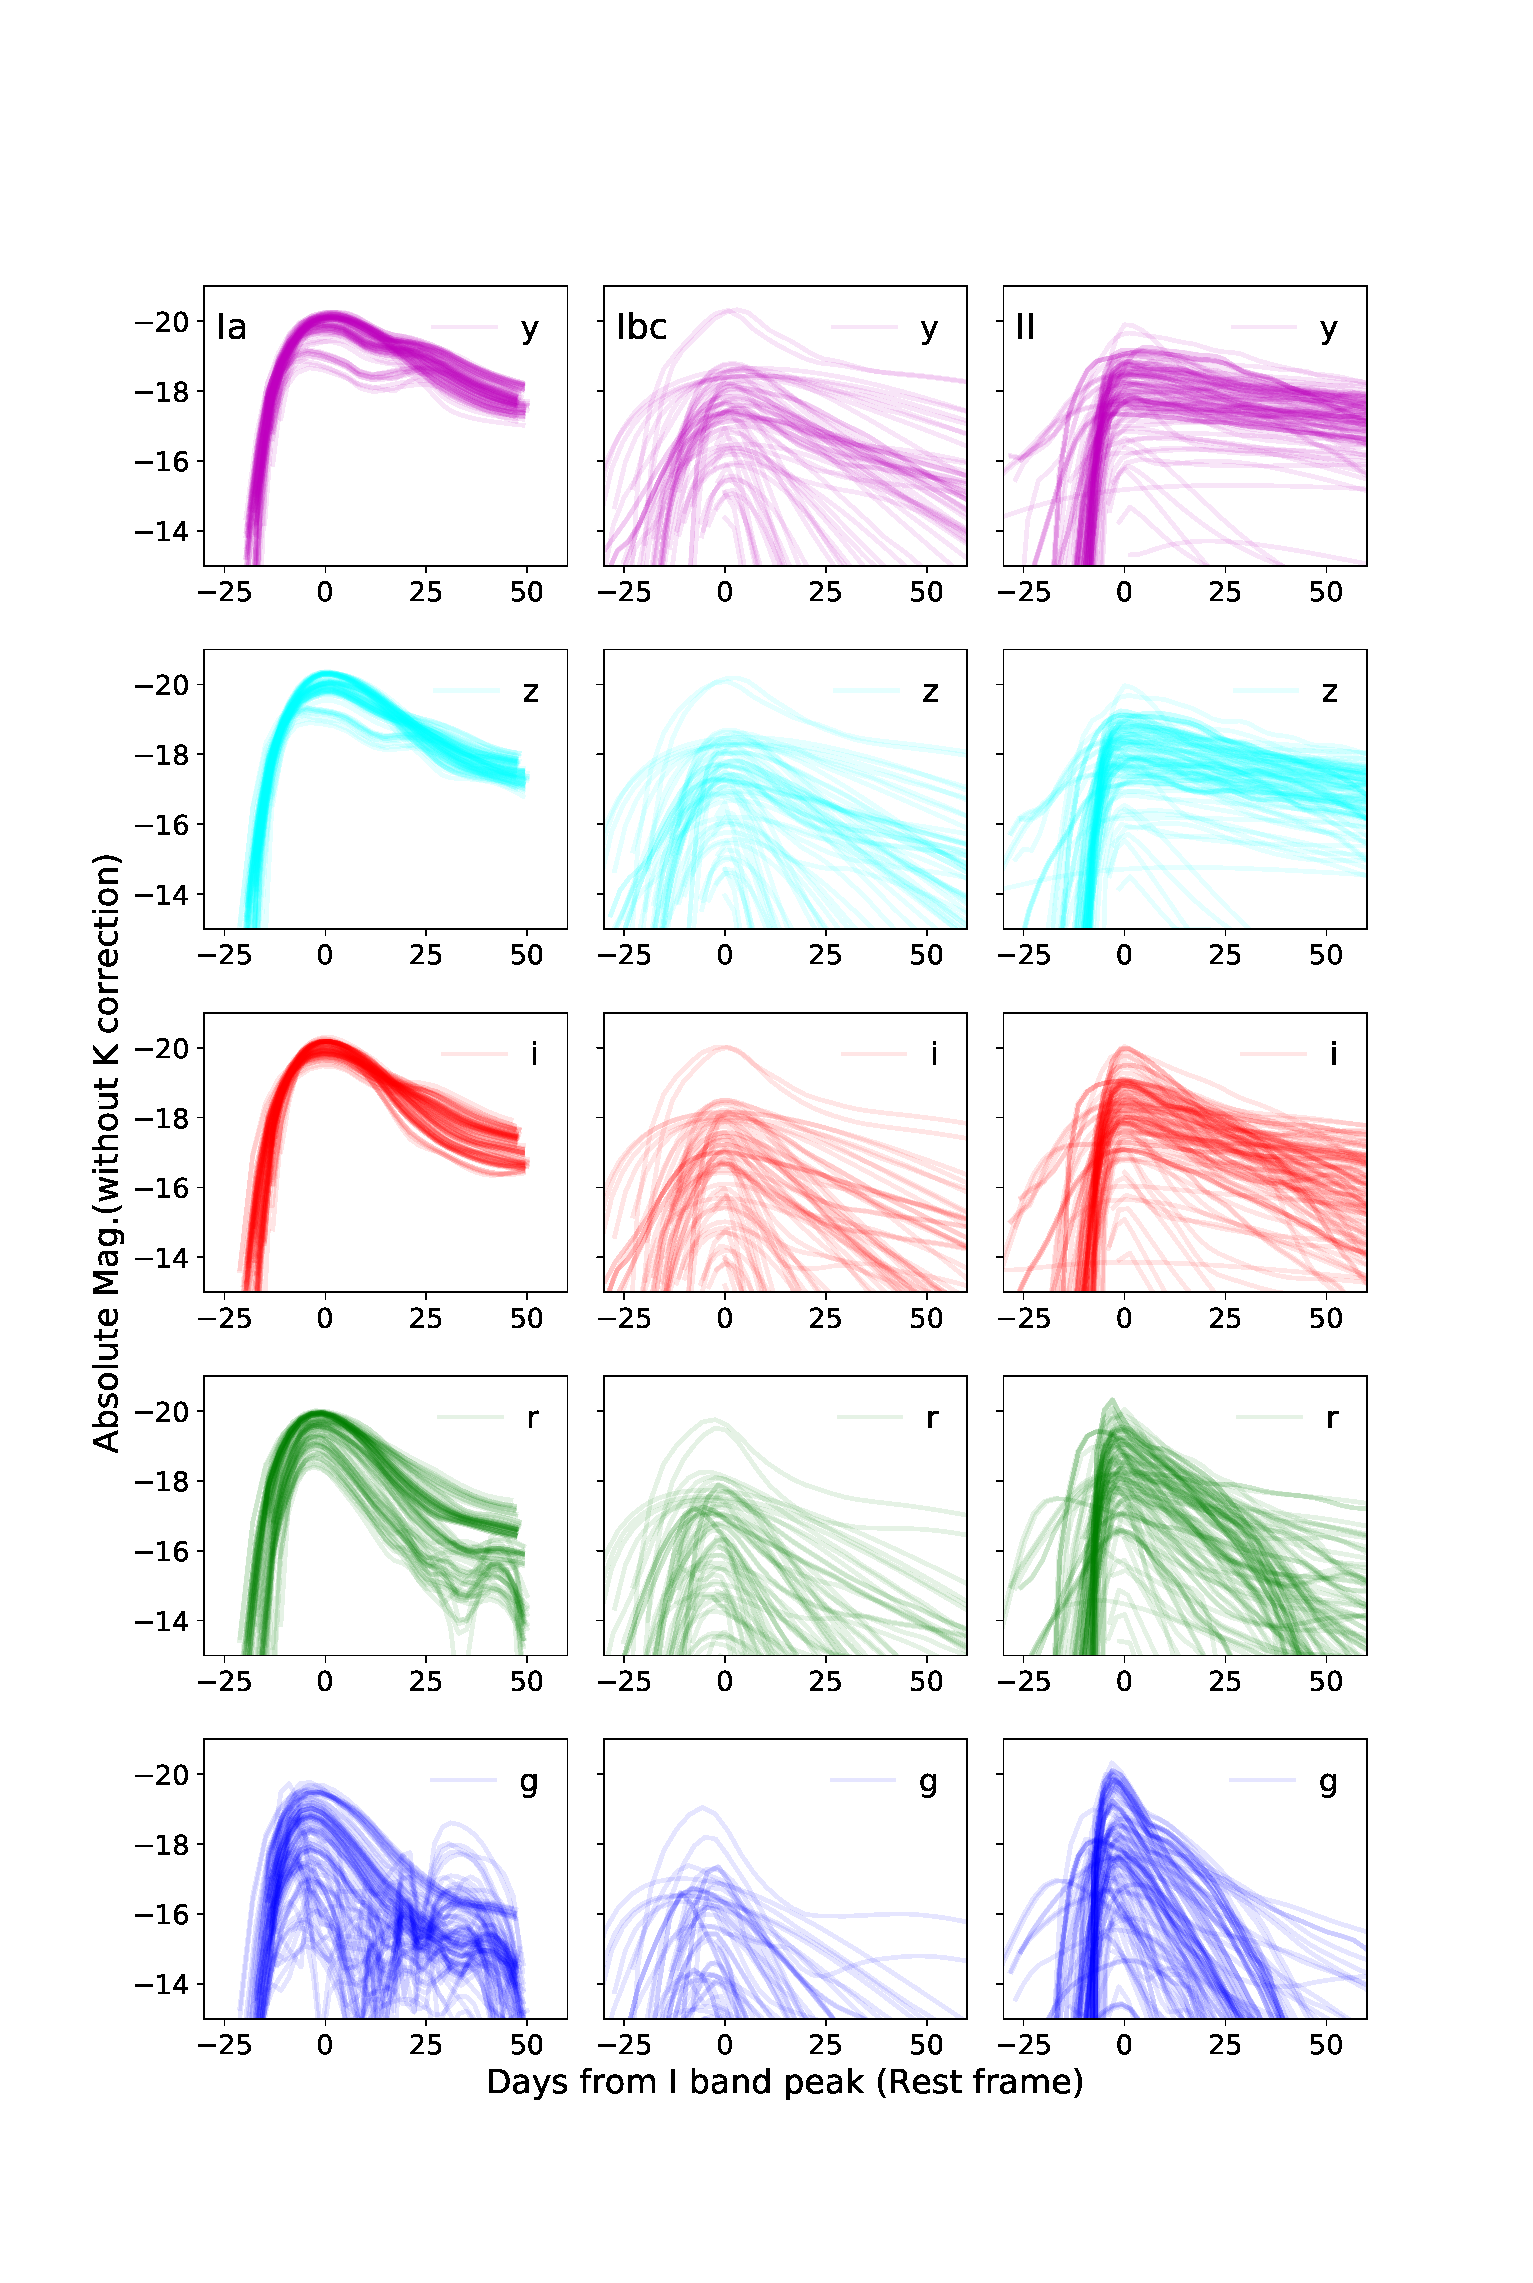
\includegraphics[width=130mm]{figures/SimLCsamples.eps}
  \end{center}
  \vspace{-6mm}
  \caption{%
  Overlay plots of simulated light curves with z between 0.1 and 1.2.
  Each panel shows the \DIFdelbeginFL \DIFdelFL{case }\DIFdelendFL \DIFaddbeginFL \DIFaddFL{plots }\DIFaddendFL of Ia, Ibc, II \DIFaddbeginFL \DIFaddFL{data }\DIFaddendFL from the left, and \DIFaddbeginFL \DIFaddFL{the }\DIFaddendFL $g$-, $r2$-, $i2$-, $z$-, $y$\DIFdelbeginFL \DIFdelFL{-band }\DIFdelendFL \DIFaddbeginFL \DIFaddFL{-bands }\DIFaddendFL from the bottom.
  The variation of the curves in each panel depends on the different parameters and templates used in the simulation.
  \DIFdelbeginFL \DIFdelFL{No }\DIFdelendFL \DIFaddbeginFL \DIFaddFL{A }\DIFaddendFL noise component \DIFdelbeginFL \DIFdelFL{is }\DIFdelendFL \DIFaddbeginFL \DIFaddFL{was not }\DIFaddendFL added to these light curves.
  }%

  \label{fig:simLCsamples}
\end{figure}
%
%
\begin{figure}[htbp]
  \begin{center}
     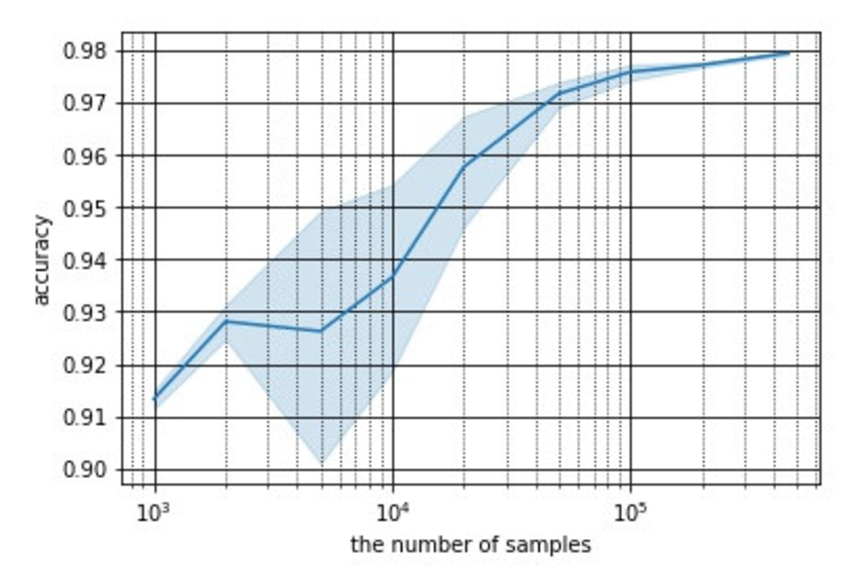
\includegraphics[width=\columnwidth]{figures/size_accuracy.eps}
  \end{center}
  \caption{%
\DIFdelbeginFL \DIFdelFL{A convergence }\DIFdelendFL \DIFaddbeginFL \DIFaddFL{Convergence }\DIFaddendFL test \DIFdelbeginFL \DIFdelFL{: We tested how many }\DIFdelendFL \DIFaddbeginFL \DIFaddFL{to determine the number of }\DIFaddendFL light curves \DIFdelbeginFL \DIFdelFL{needs }\DIFdelendFL \DIFaddbeginFL \DIFaddFL{that would need }\DIFaddendFL to be generated to train \DIFdelbeginFL \DIFdelFL{a }\DIFdelendFL \DIFaddbeginFL \DIFaddFL{the }\DIFaddendFL machine. 
The solid line shows the mean accuracy of five classifiers. The \DIFdelbeginFL \DIFdelFL{shade }\DIFdelendFL \DIFaddbeginFL \DIFaddFL{shaded }\DIFaddendFL area shows the standard deviation of the classifiers\DIFdelbeginFL \DIFdelFL{. The classifiers are }\DIFdelendFL \DIFaddbeginFL \DIFaddFL{, which were }\DIFaddendFL trained with \DIFdelbeginFL \DIFdelFL{5 fold }\DIFdelendFL \DIFaddbeginFL \DIFaddFL{5-fold }\DIFaddendFL cross validation using the training dataset. \DIFdelbeginFL \DIFdelFL{We conclude we need }\DIFdelendFL \DIFaddbeginFL \DIFaddFL{The results indicate that }\DIFaddendFL more than 100,000 light curves \DIFaddbeginFL \DIFaddFL{would be required }\DIFaddendFL for training.
  }%
  \label{fig:size_convergence_test}
\end{figure}
%

%
\subsection{Preprocessing of input data}
\label{sec:preproc}
Based on our pre-experiment with \DIFaddbegin \DIFadd{the }\DIFaddend simulated dataset, we found \DIFdelbegin \DIFdel{that the machines performs best if we 
chose }\DIFdelend \DIFaddbegin \DIFadd{the machine to perform best by using }\DIFaddend a combination of \DIFaddbegin \DIFadd{the }\DIFaddend normalized flux ($f$) and pseudo-absolute magnitude ($M$):
\begin{equation}
    x = \left( M_1^\mathrm{abs}, \ldots, M_P^\mathrm{abs}, f_{1}^{\mathrm{scale}}, \ldots, f_{P}^{\mathrm{scale}} \right)^T,
\end{equation}
where $f_{i}^{\mathrm{scale}}$ is \DIFaddbegin \DIFadd{the }\DIFaddend $i$-th raw observed flux normalized by its maximum flux:
\begin{equation}
    f_{i}^{\mathrm{scale}} = \frac{f_i}{\max \left(f_1, \ldots, f_P \right)},    \label{eq:scaled_flux}
\end{equation}
and $M_i^\mathrm{abs}$ is \DIFaddbegin \DIFadd{the }\DIFaddend $i$-th pseudo-absolute observed magnitude.
For \DIFdelbegin \DIFdel{a }\DIFdelend simplicity, we \DIFdelbegin \DIFdel{ignore }\DIFdelend \DIFaddbegin \DIFadd{ignored }\DIFaddend K-correction and \DIFdelbegin \DIFdel{use }\DIFdelend \DIFaddbegin \DIFadd{used the }\DIFaddend distance modulus (DM(z)) based on $\Lambda$CDM with \DIFaddbegin \DIFadd{the }\DIFaddend photometric redshift
from its host galaxy.
\begin{eqnarray}
    M_i^\mathrm{abs} = m_i - \mathrm{DM}\left(z\right),
\end{eqnarray}
We can justify this operation because \DIFdelbegin \DIFdel{we treat }\DIFdelend the training set and the observed dataset \DIFdelbegin \DIFdel{in the same way.
It there existed }\DIFdelend \DIFaddbegin \DIFadd{are processed using the same approach.
In the case of the existence of }\DIFaddend K-correction offset, both \DIFdelbegin \DIFdel{dataset would experience }\DIFdelend \DIFaddbegin \DIFadd{datasets would experience this }\DIFaddend in the same way.
In addition, \DIFdelbegin \DIFdel{since }\DIFdelend \DIFaddbegin \DIFadd{because }\DIFaddend the observed flux could \DIFdelbegin \DIFdel{go to }\DIFdelend \DIFaddbegin \DIFadd{take on }\DIFaddend a negative value \DIFdelbegin \DIFdel{due }\DIFdelend \DIFaddbegin \DIFadd{owing }\DIFaddend to statistical fluctuation, 
we adopt hyperbolic sine to imitate the magnitude system we use \citep{lupton99a}.  
\begin{eqnarray}
    m_i = 27.0 - \frac{2.5}{\log 10} \sinh^{-1} \frac{f_i}{2}. \label{eq:mag} 
\end{eqnarray}
In fact, \DIFdelbegin \DIFdel{the }\DIFdelend combination of the flux and magnitudes \DIFdelbegin \DIFdel{are redundant.   If we know one, we can }\DIFdelend \DIFaddbegin \DIFadd{is redundant, because knowledge of the one would enable us to }\DIFaddend calculate the other \DIFdelbegin \DIFdel{in an explicit way}\DIFdelend \DIFaddbegin \DIFadd{explicitly}\DIFaddend .   
However, based on our experiment, the score of \DIFdelbegin \DIFdel{machine gets better if we use }\DIFdelend \DIFaddbegin \DIFadd{the machine improves by using }\DIFaddend both.  
We \DIFdelbegin \DIFdel{suspect }\DIFdelend \DIFaddbegin \DIFadd{suspected that }\DIFaddend the distribution in flux (linear) \DIFdelbegin \DIFdel{and }\DIFdelend \DIFaddbegin \DIFadd{differs from that of the }\DIFaddend magnitude space (log)\DIFdelbegin \DIFdel{are different, and it gives an extra clue to the machine }\DIFdelend \DIFaddbegin \DIFadd{, which provides the machine with additional information}\DIFaddend .
Thus, we \DIFdelbegin \DIFdel{use }\DIFdelend \DIFaddbegin \DIFadd{used the }\DIFaddend pseudo-absolute magnitude ($M$) and normalized flux ($f$) as an input.

\section{Deep neural network classifier}
\label{sec:DNN}
\DIFdelbegin \DIFdel{On }\DIFdelend \DIFaddbegin \DIFadd{With }\DIFaddend the rise of \DIFdelbegin \DIFdel{the era of }\DIFdelend Big Data, the use of \DIFdelbegin \DIFdel{machine learning technique plays }\DIFdelend \DIFaddbegin \DIFadd{machine-learning techniques has played }\DIFaddend a critical role \DIFdelbegin \DIFdel{on }\DIFdelend \DIFaddbegin \DIFadd{in }\DIFaddend the analysis of astronomical data. Techniques such as \DIFdelbegin \DIFdel{Random Forest, Support Vector Machine, and Convolution Neural Network }\DIFdelend \DIFaddbegin \DIFadd{random forest, support vector machine, and convolution neural network }\DIFaddend have been used for photometric data analysis \citep{pasquet19a}, galaxy classifications \citep{hausen19a}\DIFaddbegin \DIFadd{, }\DIFaddend and spectral classifications \citep{garciadias18a,muthukrishna19c,sharma20a}.

\DIFdelbegin \DIFdel{We are in need of classifying SN }\DIFdelend \DIFaddbegin \DIFadd{In our work, we seek to classify SNe }\DIFaddend from photometric data.
\DIFdelbegin \DIFdel{We attempt to make }\DIFdelend \DIFaddbegin \DIFadd{Our approach entails making }\DIFaddend use of the observed data \DIFdelbegin \DIFdel{as it is without parameterization.
It is the Deep Learning that makes this attempt }\DIFdelend \DIFaddbegin \DIFadd{without pre-processing or parameterization.
In this regard, we rely on deep learning to make our work }\DIFaddend possible.
We \DIFdelbegin \DIFdel{test how good deep learning can do }\DIFdelend \DIFaddbegin \DIFadd{decided to test the extent to which deep learning could provide useful results }\DIFaddend without extracting features such as color, \DIFdelbegin \DIFdel{light curve width }\DIFdelend \DIFaddbegin \DIFadd{the width of the light curve, }\DIFaddend and the peak magnitude\DIFdelbegin \DIFdel{on this paper}\DIFdelend .

\DIFdelbegin \DIFdel{We push }\DIFdelend \DIFaddbegin \DIFadd{The fact that we went }\DIFaddend one step further \DIFdelbegin \DIFdel{and use }\DIFdelend \DIFaddbegin \DIFadd{by leaving }\DIFaddend the observed data as raw as possible, \DIFdelbegin \DIFdel{meaning our input is }\DIFdelend \DIFaddbegin \DIFadd{means that our input consists of }\DIFaddend a simple array of magnitudes. \DIFdelbegin \DIFdel{Such attempt would not be }\DIFdelend \DIFaddbegin \DIFadd{An attempt such as this would not have been }\DIFaddend possible ten years ago\DIFdelbegin \DIFdel{, but thanks for the advancement of computing and }\DIFdelend \DIFaddbegin \DIFadd{; however, owing to advancements in computing and the }\DIFaddend deep learning technique, \DIFdelbegin \DIFdel{now it becomes a }\DIFdelend \DIFaddbegin \DIFadd{this has become }\DIFaddend reality. Among \DIFdelbegin \DIFdel{many other machine learning methods, }\DIFdelend \DIFaddbegin \DIFadd{the many machine-learning methods, we decided to use a }\DIFaddend deep neural network \DIFdelbegin \DIFdel{is our choice which enables }\DIFdelend \DIFaddbegin \DIFadd{to enable }\DIFaddend us to classify astronomical objects from the raw observed data. 

\subsection{Model design}
\label{sec:model} %added by IT
In this section, we describe \DIFdelbegin \DIFdel{our design of DNN model
}\DIFdelend \DIFaddbegin \DIFadd{the design of our DNN model,
}\DIFaddend \footnote{The code for our model is available at $\langle$https://github.com/ichiro-takahashi/snclass$\rangle$.}
which \DIFdelbegin \DIFdel{takes }\DIFdelend \DIFaddbegin \DIFadd{accepts }\DIFaddend an array of observed magnitudes as \DIFdelbegin \DIFdel{an }\DIFdelend \DIFaddbegin \DIFadd{its }\DIFaddend input and outputs \DIFaddbegin \DIFadd{the }\DIFaddend SN classification with probabilities. We adopted \DIFdelbegin \DIFdel{Highway layer \citep{srivastava15a} }\DIFdelend \DIFaddbegin \DIFadd{a highway layer (also known as a ``layer in layer'' \citep{srivastava15a}) }\DIFaddend as a core part of our network\DIFdelbegin \DIFdel{which is also called 'layer in layer'}\DIFdelend . Compared to \DIFdelbegin \DIFdel{the }\DIFdelend plain DNN, \DIFdelbegin \DIFdel{Highway layer can perform better }\DIFdelend \DIFaddbegin \DIFadd{the performance of a highway layer improves }\DIFaddend when the network is deep in terms of parameter optimization \citep{srivastava15b}.   
\DIFdelbegin \DIFdel{Just like }\DIFdelend \DIFaddbegin \DIFadd{Similar to }\DIFaddend other DNN models, this model \DIFdelbegin \DIFdel{goes through training, }\DIFdelend \DIFaddbegin \DIFadd{proceeds through a training and }\DIFaddend validation process to optimize \DIFaddbegin \DIFadd{the }\DIFaddend parameters, and we describe the steps below. \DIFdelbegin \DIFdel{The terminology we use is common }\DIFdelend \DIFaddbegin \DIFadd{Our terminology is commonly used }\DIFaddend in the world of DNN, but \DIFaddbegin \DIFadd{as }\DIFaddend this is a new introduction to \DIFaddbegin \DIFadd{the }\DIFaddend astronomical community, we \DIFdelbegin \DIFdel{spell out each step one by one}\DIFdelend \DIFaddbegin \DIFadd{explain each step in detail}\DIFaddend . The architecture of our model is summarized in figure \ref{fig:dnn_model}.
\DIFdelbegin \DIFdel{At the end}\DIFdelend \DIFaddbegin \DIFadd{Ultimately}\DIFaddend , each SN is \DIFdelbegin \DIFdel{given }\DIFdelend \DIFaddbegin \DIFadd{assigned }\DIFaddend a probability of \DIFdelbegin \DIFdel{being }\DIFdelend \DIFaddbegin \DIFadd{belonging to }\DIFaddend a certain astrophysical class, in our case, \DIFdelbegin \DIFdel{SN types}\DIFdelend \DIFaddbegin \DIFadd{the type of SN}\DIFaddend . 
%
\begin{figure}[htbp]
  \begin{center}
    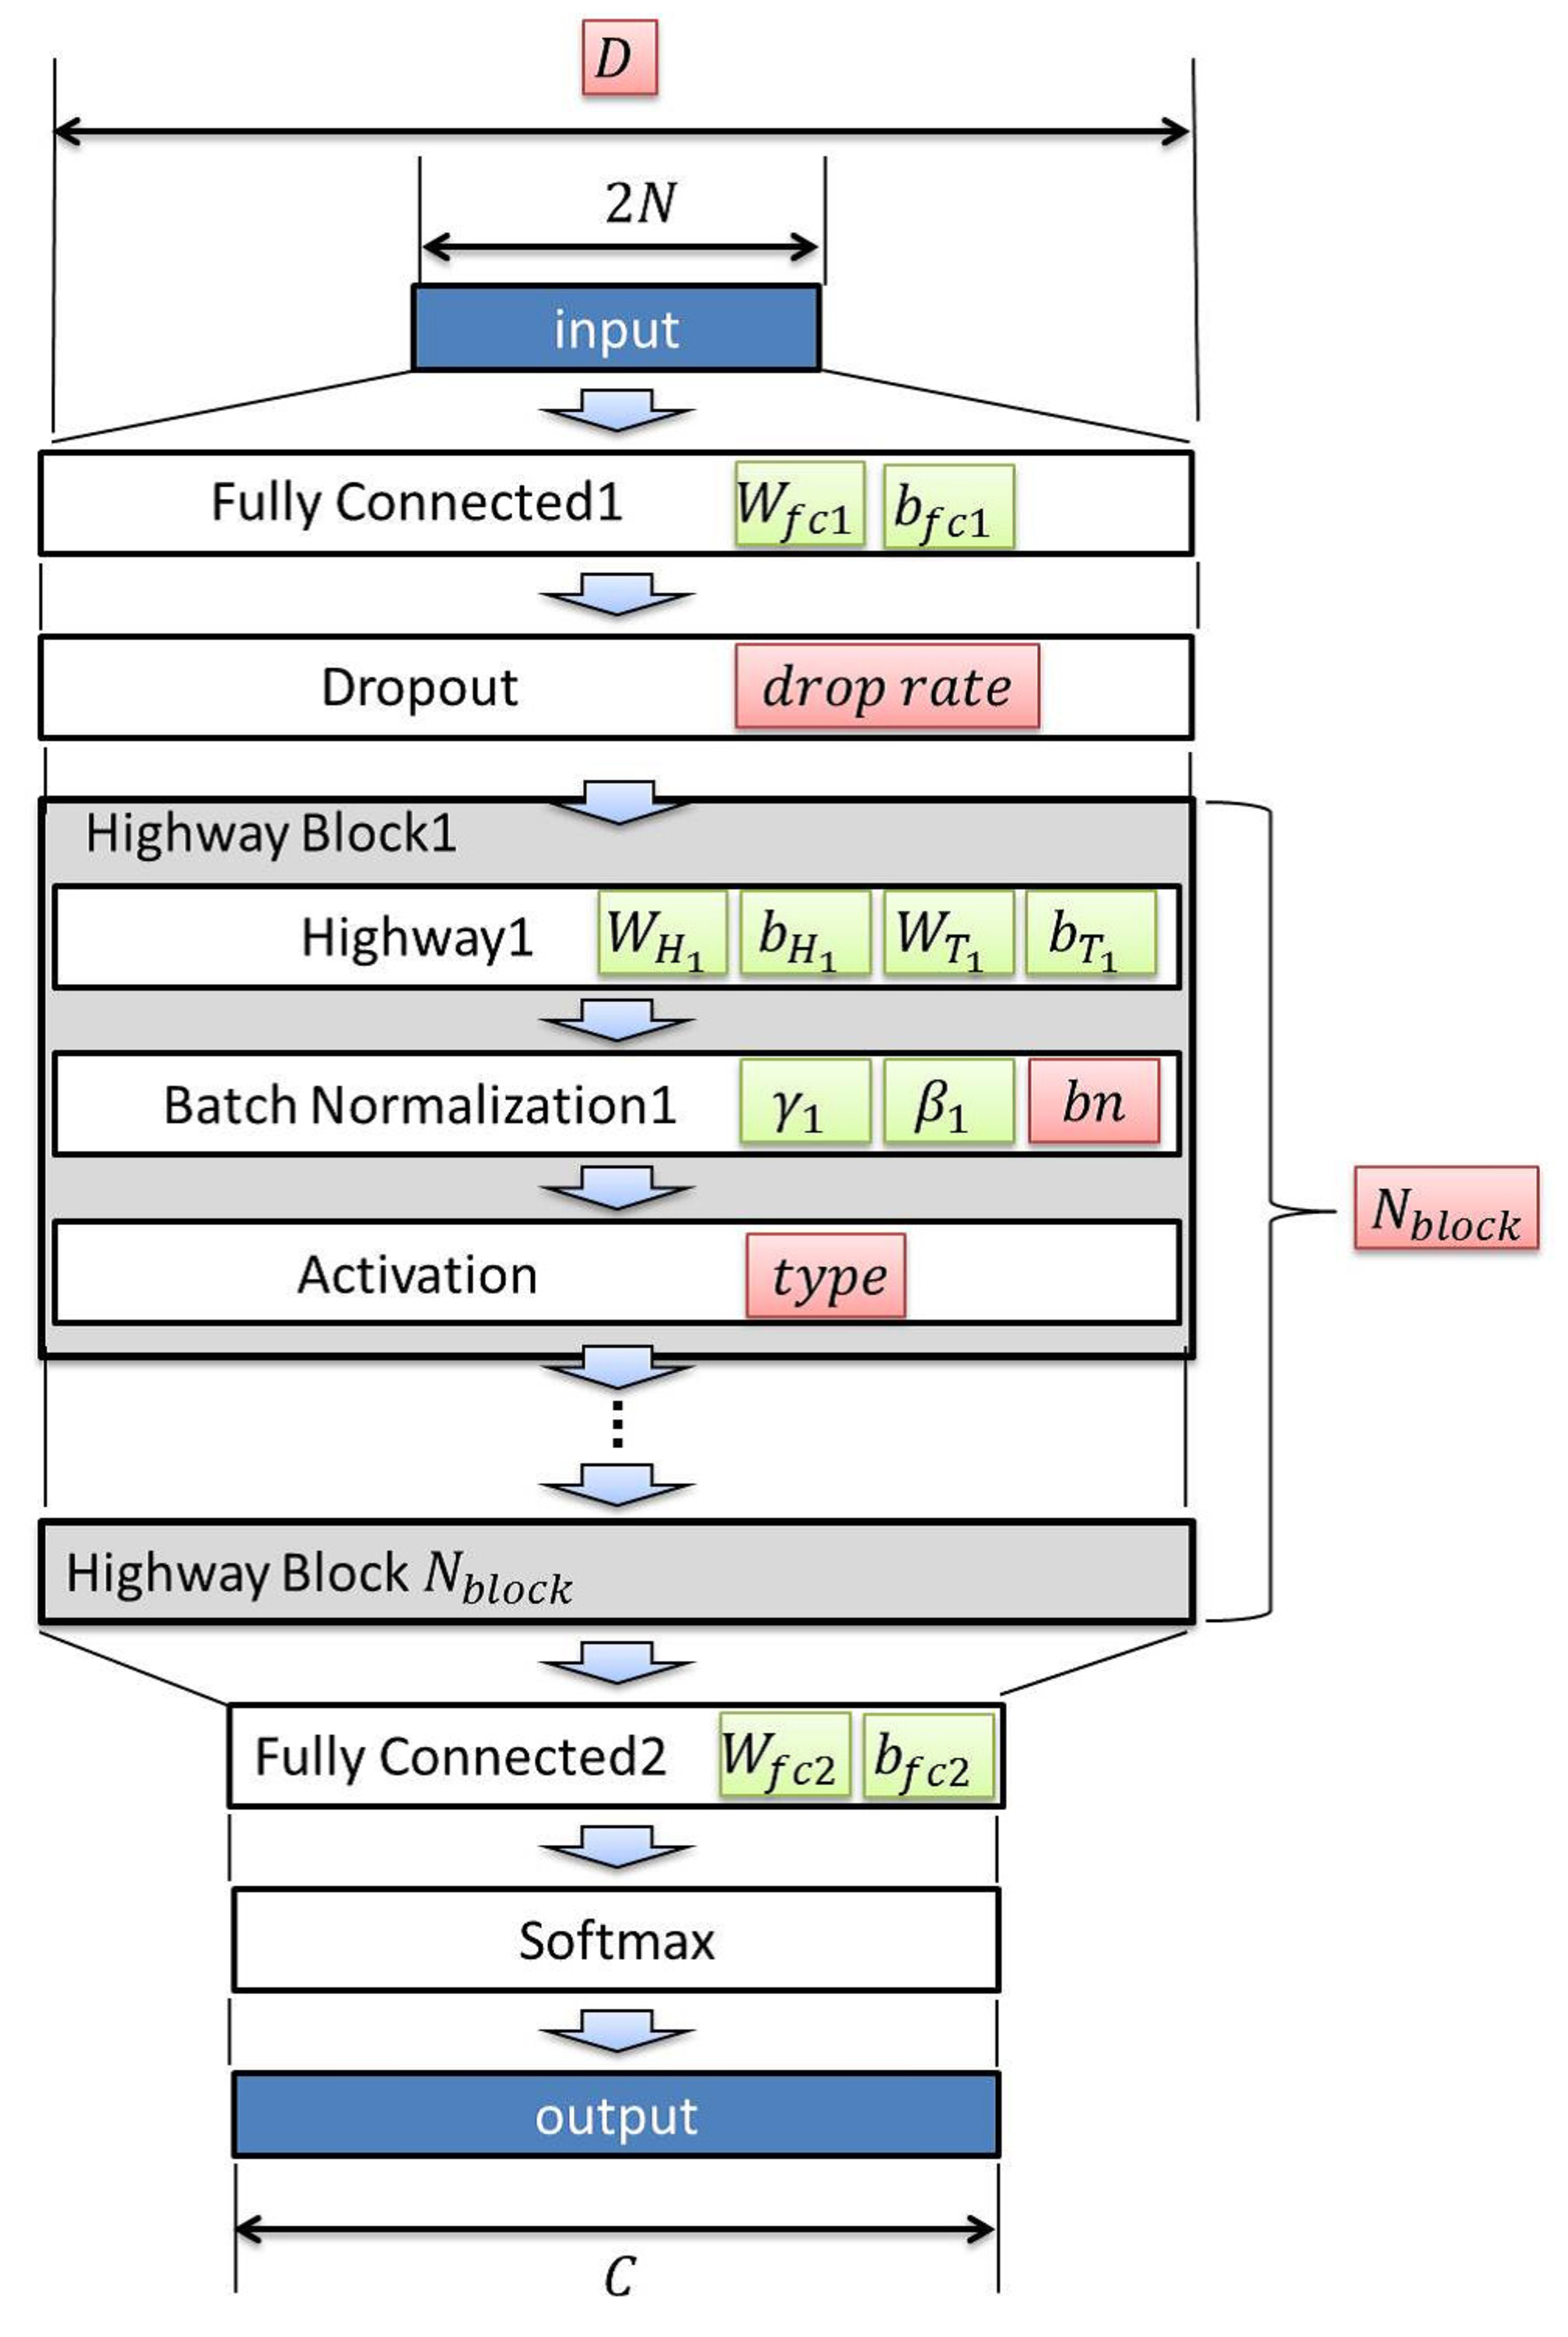
\includegraphics[width=130mm]{figures/model_all.eps}
  \end{center}
  \caption{\label{dnnmodel}
  \DIFdelbeginFL \DIFdelFL{The architecture }\DIFdelendFL \DIFaddbeginFL \DIFaddFL{Architecture }\DIFaddendFL of the deep neural network classifier. 
  The green boxes are parameters \DIFdelbeginFL \DIFdelFL{which are }\DIFdelendFL optimized by \DIFaddbeginFL \DIFaddFL{the }\DIFaddendFL gradient descent method during training. The red boxes are \DIFdelbeginFL \DIFdelFL{hyper-parameters which }\DIFdelendFL \DIFaddbeginFL \DIFaddFL{hyperparameters that }\DIFaddendFL are optimized \DIFdelbeginFL \DIFdelFL{by }\DIFdelendFL \DIFaddbeginFL \DIFaddFL{during }\DIFaddendFL the \DIFdelbeginFL \DIFdelFL{hyper-parameter }\DIFdelendFL \DIFaddbeginFL \DIFaddFL{hyperparameter }\DIFaddendFL search. 
  \DIFdelbeginFL \DIFdelFL{Batch Normalization }\DIFdelendFL \DIFaddbeginFL \DIFaddFL{The batch normalization }\DIFaddendFL layer has four variables ($\mu, \sigma^2, \gamma, \beta$)\DIFdelbeginFL \DIFdelFL{. }\DIFdelendFL \DIFaddbeginFL \DIFaddFL{, where }\DIFaddendFL $\mu$ and $\sigma^2$ are \DIFaddbeginFL \DIFaddFL{intended }\DIFaddendFL to learn the statistics (mean and variance) of the value through the layer\DIFaddbeginFL \DIFaddFL{, }\DIFaddendFL respectively\DIFdelbeginFL \DIFdelFL{.  }\DIFdelendFL \DIFaddbeginFL \DIFaddFL{, and }\DIFaddendFL $\gamma$ and $\beta$ are scale \DIFdelbeginFL \DIFdelFL{parameter }\DIFdelendFL and shift \DIFdelbeginFL \DIFdelFL{parameter }\DIFdelendFL \DIFaddbeginFL \DIFaddFL{parameters, respectively, }\DIFaddendFL to adjust the output. \DIFaddbeginFL \DIFaddFL{Note that }\DIFaddendFL $\mu$ and $\sigma^2$ are not updated by gradient descent\DIFdelbeginFL \DIFdelFL{method but }\DIFdelendFL \DIFaddbeginFL \DIFaddFL{; instead, they }\DIFaddendFL are updated by \DIFaddbeginFL \DIFaddFL{the }\DIFaddendFL moving average. \DIFdelbeginFL \DIFdelFL{We omit them }\DIFdelendFL \DIFaddbeginFL \DIFaddFL{They were omitted }\DIFaddendFL from the figure for simplicity.
  }%
  \label{fig:dnn_model}
\end{figure}
%


{\bf Input}: Our input is an array of magnitudes and normalized fluxes of the $i$th SN in the training \DIFdelbegin \DIFdel{data set:
}\DIFdelend \DIFaddbegin \DIFadd{dataset:
}\DIFaddend \begin{equation}
      x_i = \left( M_{i1}, M_{i2}, \ldots M_{ij} \ldots , M_{iN}, f_{i1}, f_{i2}, \ldots, f_{iN} \right)^T\DIFaddbegin \DIFadd{.
}\DIFaddend \end{equation}
We do not \DIFdelbegin \DIFdel{use time or filter explicitly but it }\DIFdelend \DIFaddbegin \DIFadd{explicitly specify the time at which or the particular filter with which the data were recorded, but this information }\DIFaddend is recorded as an order inside the array. The philosophy here is that the training set\DIFaddbegin \DIFadd{, }\DIFaddend which is composed of \DIFdelbegin \DIFdel{the simulated data in }\DIFdelend \DIFaddbegin \DIFadd{simulated data of }\DIFaddend the same array length\DIFdelbegin \DIFdel{holds the information on }\DIFdelend \DIFaddbegin \DIFadd{, includes information on the }\DIFaddend filter and dates. For example, the $j$th magnitude in the array is \DIFdelbegin \DIFdel{the data taken }\DIFdelend \DIFaddbegin \DIFadd{data recorded }\DIFaddend on a certain date and by a certain filter. The combination of the date and filter is identical to \DIFdelbegin \DIFdel{the ones }\DIFdelend \DIFaddbegin \DIFadd{those }\DIFaddend in the training set. Therefore, the $j$th component implicitly contains unique information about \DIFaddbegin \DIFadd{the }\DIFaddend dates and filters.  
\DIFdelbegin \DIFdel{If input is }\DIFdelend \DIFaddbegin \DIFadd{Considering that the input consists of }\DIFaddend a combination of \DIFaddbegin \DIFadd{the }\DIFaddend magnitude and normalized flux,
\DIFaddbegin \DIFadd{The size of }\DIFaddend our input array \DIFdelbegin \DIFdel{has a size of }\DIFdelend \DIFaddbegin \DIFadd{is }\DIFaddend $1\times2N$ per \DIFdelbegin \DIFdel{a }\DIFdelend SN where $N$ is the number of data points.


{\bf First Fully Connected layer:}
We \DIFdelbegin \DIFdel{would like }\DIFdelend \DIFaddbegin \DIFadd{decided }\DIFaddend to make use of $D$ neurons\DIFdelbegin \DIFdel{which is }\DIFdelend \DIFaddbegin \DIFadd{, }\DIFaddend also known as the number of \DIFdelbegin \DIFdel{'hidden layer',}\DIFdelend \DIFaddbegin \DIFadd{``hidden layers,'' }\DIFaddend and $D$ is greater than the number of input components ($2N$). However, the dimension \DIFaddbegin \DIFadd{of }\DIFaddend $D$ is not known in advance, and this \DIFdelbegin \DIFdel{parameter }\DIFdelend is one of the hyperparameters we optimize later in this section. \DIFdelbegin \DIFdel{Since the dimension of }\DIFdelend \DIFaddbegin \DIFadd{Because the dimensionality of the }\DIFaddend input ($2N$) \DIFdelbegin \DIFdel{and }\DIFdelend \DIFaddbegin \DIFadd{could differ from }\DIFaddend the number of optimized neurons $D$\DIFdelbegin \DIFdel{could be different, we are in need of adjusting the }\DIFdelend \DIFaddbegin \DIFadd{, we would need to adjust the number of }\DIFaddend dimensions and that is the role of this \DIFdelbegin \DIFdel{First Fully Connected }\DIFdelend \DIFaddbegin \DIFadd{first fully connected }\DIFaddend layer $F(x)$.    
\begin{equation}
    F \left(x, \left\{W_{fc1},b_{fc1}\right\}\right) = W_{fc1} x + b_{fc1} \in \mathbb{R}^D.
\end{equation}
$F(x)$ is given by a linear combination of matrix $W_{fc} \in \mathbb{R}^{D\times 2N}$ and a vector $b_{fc} \in \mathbb{R}^D$. The initial value of $W_{fc}$ is generated by Gaussian distribution and $b_{fc}$ is initialized by $\mathbf{0}$, which is a $D$\DIFdelbegin \DIFdel{dimentional vector and the all }\DIFdelend \DIFaddbegin \DIFadd{-dimensional vector of which all the }\DIFaddend elements are zero. We \DIFdelbegin \DIFdel{use a python wrapper library called }\DIFdelend \DIFaddbegin \DIFadd{used the Python wrapper library }\DIFaddend {\it dm-sonnet} \DIFaddbegin \DIFadd{(version 1.23)
}\DIFaddend %added 200708
\footnote{{\it dm-sonnet} $\langle$https://github.com/deepmind/sonnet$\rangle$.}
%
and its function \DIFdelbegin \DIFdel{called }\DIFdelend {\it linear} \DIFdelbegin \DIFdel{supplies }\DIFdelend \DIFaddbegin \DIFadd{to supply }\DIFaddend the $F(x)$ when \DIFdelbegin \DIFdel{we plug in '}\DIFdelend \DIFaddbegin \DIFadd{plugging in ``}\DIFaddend $2N$\DIFdelbegin \DIFdel{' and '}\DIFdelend \DIFaddbegin \DIFadd{'' and ``}\DIFaddend $D$\DIFdelbegin \DIFdel{'.Later on}\DIFdelend \DIFaddbegin \DIFadd{.''  
Subsequently}\DIFaddend , $W_{fc}$ and $b_{fc}$ are \DIFdelbegin \DIFdel{optimised by an open source Machine Learning package , }\DIFdelend \DIFaddbegin \DIFadd{optimized by the open source machine-learning package }\DIFaddend {\it Tensorflow} \DIFaddbegin \DIFadd{(version 1.14) }\DIFaddend \citep{Abadi2016}.  
%added 200707
\DIFdelbegin \DIFdel{The versions of }%DIFDELCMD < {\it %%%
\DIFdel{dm-sonnet}%DIFDELCMD < } %%%
\DIFdel{and }%DIFDELCMD < {\it %%%
\DIFdel{Tensorflow}%DIFDELCMD < } %%%
\DIFdel{used are 1.23 and 1.14 respectively.
}\DIFdelend %
Unless \DIFdelbegin \DIFdel{we mention }\DIFdelend \DIFaddbegin \DIFadd{stated }\DIFaddend otherwise, we \DIFdelbegin \DIFdel{use }\DIFdelend \DIFaddbegin \DIFadd{used the }\DIFaddend libraries from {\it Tensorflow}.

{\bf Dropout layer:}
\DIFdelbegin \DIFdel{In order to have }\DIFdelend \DIFaddbegin \DIFadd{To obtain }\DIFaddend a robust result, it is always best to train all of the neurons as an ensemble and avoid \DIFaddbegin \DIFadd{a situation in which }\DIFaddend one of the neurons \DIFdelbegin \DIFdel{drags }\DIFdelend \DIFaddbegin \DIFadd{adversely affects }\DIFaddend the result. Dropout is a process \DIFdelbegin \DIFdel{which randomly drops some of the neurons from the }\DIFdelend \DIFaddbegin \DIFadd{in which certain neurons are randomly dropped from }\DIFaddend training and the \DIFdelbegin \DIFdel{rate of dropout }\DIFdelend \DIFaddbegin \DIFadd{dropout rate }\DIFaddend can be optimized as one of the hyperparameters \citep{dropout}. 

{\bf Highway layer:}
We adopted \DIFaddbegin \DIFadd{a }\DIFaddend Highway layer \citep{srivastava15a} and \DIFaddbegin \DIFadd{optimized }\DIFaddend the number of layers \DIFdelbegin \DIFdel{is optimized through }\DIFdelend \DIFaddbegin \DIFadd{therein during the }\DIFaddend hyperparameter search. In theory, \DIFdelbegin \DIFdel{we can }\DIFdelend \DIFaddbegin \DIFadd{it would be possible to }\DIFaddend design a very deep \DIFdelbegin \DIFdel{layer and the number of layers can be more than we need. In fact, }\DIFdelend \DIFaddbegin \DIFadd{highway layer with more layers than would be necessary. However, in reality, }\DIFaddend it is not trivial to \DIFdelbegin \DIFdel{find the optimized }\DIFdelend \DIFaddbegin \DIFadd{optimize the }\DIFaddend number of layers.   
The depth and/or \DIFdelbegin \DIFdel{layer }\DIFdelend size of the \DIFdelbegin \DIFdel{DNN model is }\DIFdelend \DIFaddbegin \DIFadd{layers of the DNN model are }\DIFaddend directly related to the complexity of the features \DIFdelbegin \DIFdel{that we }\DIFdelend \DIFaddbegin \DIFadd{used as }\DIFaddend input, and greatly affect the \DIFaddbegin \DIFadd{computational }\DIFaddend performance of the task.  
\DIFdelbegin \DIFdel{However, if a model is too deep , }\DIFdelend \DIFaddbegin \DIFadd{Thus, an overly deep model would complicate }\DIFaddend the learning process \DIFdelbegin \DIFdel{becomes difficult and causes }\DIFdelend \DIFaddbegin \DIFadd{and cause }\DIFaddend performance degradation.
\DIFdelbegin \DIFdel{Highway }\DIFdelend \DIFaddbegin \DIFadd{A highway }\DIFaddend layer is a technique that stabilizes \DIFaddbegin \DIFadd{the }\DIFaddend learning process by devising the network structure.
\DIFdelbegin \DIFdel{In \citet{Kimura17}, we have used Highway layerand }\DIFdelend \DIFaddbegin \DIFadd{We previously used a highway layer, which we }\DIFaddend tested on 2D \DIFdelbegin \DIFdel{image}\DIFdelend \DIFaddbegin \DIFadd{images}\DIFaddend , and it \DIFdelbegin \DIFdel{proved a good performance .  The details }\DIFdelend \DIFaddbegin \DIFadd{delivered good performance \citet{Kimura17}. Details }\DIFaddend of the use and \DIFdelbegin \DIFdel{the advantages of Highway layer is described in \citet{Kimura17}.  We continue to adopt Highway }\DIFdelend \DIFaddbegin \DIFadd{advantages of the highway layer are provided in a previous paper of ours \citet{Kimura17}. This encouraged us to adopt a highway }\DIFaddend layer scheme for this analysis.
The output of \DIFdelbegin \DIFdel{Highway }\DIFdelend \DIFaddbegin \DIFadd{the highway }\DIFaddend layer is calculated from the values of \DIFdelbegin \DIFdel{the }\DIFdelend multiple paths.
The output, ${\bf Highway} \left(x\right)$, is formulated as
\begin{equation}
    {\bf Highway} \left(x\right) = G \left(x\right) \otimes H \left(x\right) + C \left(x\right) \otimes x \in \mathbb{R}^D,
\end{equation}
where $H$ is a \DIFdelbegin \DIFdel{non-linear transformation layer. }\DIFdelend \DIFaddbegin \DIFadd{nonlinear transformation layer, }\DIFaddend $G$ is the transformation gate function layer and controls the transformation of input\DIFdelbegin \DIFdel{.  }\DIFdelend \DIFaddbegin \DIFadd{, }\DIFaddend $C$ is the carry gate function layer\DIFdelbegin \DIFdel{. The symbol, }\DIFdelend \DIFaddbegin \DIFadd{, and }\DIFaddend $\otimes$ \DIFdelbegin \DIFdel{, is }\DIFdelend \DIFaddbegin \DIFadd{provides the }\DIFaddend element-wise product, also known as \DIFaddbegin \DIFadd{the }\DIFaddend Hadamard product.
\DIFdelbegin \DIFdel{Highway layer includes other layers inside.  This structure is called }\DIFdelend \DIFaddbegin \DIFadd{A highway layer includes several other layers, a structure known as ``}\DIFaddend layer in layer.\DIFaddbegin \DIFadd{'' }\DIFaddend Each function is defined as follows: 
\begin{eqnarray}
    H \left(x\right) &=& \mathrm{a} \left( F \left(x, \left\{W_{H_{fc}}, b_{H_{fc}}\right\}\right) \right) \in \mathbb{R}^D, \\
    G \left(x\right) &=& \mathrm{a} \left( F \left(x, \left\{W_{G_{fc}}, b_{G_{fc}}\right\}\right) \right) \in \mathbb{R}^D, \\
    C \left(x\right) &=& \mathbf{1} - G \left(x\right) \in \mathbb{R}^D,
\end{eqnarray}
where $a$ is an activation function, namely\DIFaddbegin \DIFadd{, }\DIFaddend sigmoid.
\begin{eqnarray*}
    \mathrm{a} \left(p\right) &=& \left( \sigma\left(p_1\right),\sigma\left(p_2\right), \ldots, \sigma\left(p_D\right) \right)^T, \; p \in \mathbb{R}^D, \\
    \sigma \left(p_i\right) &=& \frac{1}{1 + e^{-p_i}},
\end{eqnarray*}
\DIFdelbegin \DIFdel{Note }\DIFdelend \DIFaddbegin \DIFadd{where }\DIFaddend $D$ is the number of neurons. Each element of $G(x)$ always takes a value between 0 and 1. \DIFdelbegin \DIFdel{At the end values, }\DIFdelend \DIFaddbegin \DIFadd{Eventually, the }\DIFaddend Highway layer behaves as follows:
\begin{equation}
    {\bf Highway(x)}=\left\{
    \begin{array}{@{}ll@{}}
    %\begin{cases}
      x, & \mathrm{if} \ G \left(x\right)= \mathbf{0} \\
      H(x), & \mathrm{if} \ G \left(x\right)= \mathbf{1} 
    %\end{cases}
    \end{array}\right.
\end{equation}
Along with the \DIFdelbegin \DIFdel{hidden layer dimensions }\DIFdelend \DIFaddbegin \DIFadd{dimensions of the hidden layer }\DIFaddend $D$, the dropout ratio, batch normalization, and the types of activation function, the number of \DIFdelbegin \DIFdel{repetition }\DIFdelend \DIFaddbegin \DIFadd{repetitions }\DIFaddend $T$ is one of the hyperparameters and \DIFdelbegin \DIFdel{optimized through }\DIFdelend \DIFaddbegin \DIFadd{is optimized by performing a }\DIFaddend hyperparameter search. \DIFdelbegin \DIFdel{The details are described }\DIFdelend \DIFaddbegin \DIFadd{Details are provided }\DIFaddend in subsection \ref{hyperparametersearch}.

{\bf Batch \DIFdelbegin \DIFdel{Normalization }\DIFdelend \DIFaddbegin \DIFadd{normalization }\DIFaddend layer:}
We adopt \DIFdelbegin \DIFdel{Batch Normalization }\DIFdelend \DIFaddbegin \DIFadd{batch normalization }\DIFaddend \citep{batch_norm} to accelerate and stabilize the optimization. Even if \DIFdelbegin \DIFdel{it may be }\DIFdelend a large number of parameters \DIFdelbegin \DIFdel{we need to train, Batch Normalization helps converge the training , reduce }\DIFdelend \DIFaddbegin \DIFadd{need to be trained, batch normalization facilitates convergence of the training process, reduces }\DIFaddend errors on the slope when we apply entropy minimization, prevents the average and dispersion \DIFdelbegin \DIFdel{goes }\DIFdelend \DIFaddbegin \DIFadd{from becoming }\DIFaddend exponentially large in deep layers, and \DIFdelbegin \DIFdel{minimize }\DIFdelend \DIFaddbegin \DIFadd{minimizes }\DIFaddend the biases on outputs \citep{understanding_batch_norm}.
Batch \DIFdelbegin \DIFdel{Normalization works well }\DIFdelend \DIFaddbegin \DIFadd{normalization is effective }\DIFaddend in many cases. However, \DIFdelbegin \DIFdel{if both Batch Normalization and Dropout are in the model, the performance }\DIFdelend \DIFaddbegin \DIFadd{the performance of a model that employs both batch normalization and dropout }\DIFaddend may degrade (\cite{dropout_and_batch_norm}).   

{\bf Activation layer:}
Each neuron is activated \DIFdelbegin \DIFdel{through a non-linear transformation. Non-linearity }\DIFdelend \DIFaddbegin \DIFadd{by using nonlinear transformation. Nonlinearity }\DIFaddend is an important component \DIFdelbegin \DIFdel{for DNNwhich gives us }\DIFdelend \DIFaddbegin \DIFadd{of DNN, because it allows }\DIFaddend a wide variety of \DIFdelbegin \DIFdel{expression. Note }\DIFdelend \DIFaddbegin \DIFadd{expressions. Note that }\DIFaddend the majority of the layers, including \DIFdelbegin \DIFdel{Fully Connected Layers, are }\DIFdelend \DIFaddbegin \DIFadd{fully connected layers, involve }\DIFaddend a linear transformation and\DIFdelbegin \DIFdel{even if we have }\DIFdelend \DIFaddbegin \DIFadd{, even if }\DIFaddend a number of layers \DIFdelbegin \DIFdel{, it is equivalent of }\DIFdelend \DIFaddbegin \DIFadd{were to exist, it would be equivalent to }\DIFaddend one single linear transformation. Thus, \DIFdelbegin \DIFdel{it }\DIFdelend \DIFaddbegin \DIFadd{nonlinear transformation }\DIFaddend is essential to \DIFdelbegin \DIFdel{have a non-linear transformation so that each neuron can have a freedom to take any values necessary }\DIFdelend \DIFaddbegin \DIFadd{allow each neuron the freedom to have any necessary values}\DIFaddend .
For the first iteration, we do not know what kind of transformation is the best\DIFaddbegin \DIFadd{; thus}\DIFaddend , the transformation itself is taken as one of the hyperparameters. \DIFdelbegin \DIFdel{The functions, '}\DIFdelend \DIFaddbegin \DIFadd{In our work, we used the functions ``}\DIFaddend tf.nn\DIFdelbegin \DIFdel{',}\DIFdelend \DIFaddbegin \DIFadd{,'' }\DIFaddend in {\it Tensorflow}\DIFdelbegin \DIFdel{is being used}\DIFdelend .

{\bf Second \DIFdelbegin \DIFdel{Fully Connected }\DIFdelend \DIFaddbegin \DIFadd{fully connected }\DIFaddend layer:}
After $T$ \DIFdelbegin \DIFdel{reptitions of Highway layer, Batch Normalization }\DIFdelend \DIFaddbegin \DIFadd{repetitions of the highway layer, batch normalization }\DIFaddend layer, and \DIFdelbegin \DIFdel{Activation layer,
we are in need of converting }\DIFdelend \DIFaddbegin \DIFadd{activation layer,
it is necessary to convert }\DIFaddend the number of neurons to the number of SNe times the number of SN classes. This \DIFdelbegin \DIFdel{is an opposite operation of the First Fully Connected layers}\DIFdelend \DIFaddbegin \DIFadd{operation is opposite to that of the first fully connected layer}\DIFaddend .

{\bf Softmax layer:}
\DIFdelbegin \DIFdel{Softmax layer normalize }\DIFdelend \DIFaddbegin \DIFadd{The Softmax layer normalizes }\DIFaddend the input value of this layer, which is denoted by $h \in \mathbb{R}^D$. The output value is $\hat{y} \in \mathbb{R}^D$ and each element $\hat{y}_k$ is expressed as
\begin{equation}
    \hat{y}_k = \frac{\exp \left( h_k \right)}{\sum_{k'=1}^K \exp \left( h_{k'} \right)}.
\end{equation}
The normalized value $\hat{y}$ satisfies $\hat{y}_k \geq 0$ and $\sum_k^K \hat{y}_k =1$.
We can interpret $\hat{y}_k$ as \DIFdelbegin \DIFdel{a }\DIFdelend \DIFaddbegin \DIFadd{the }\DIFaddend probability that the input $x$ belongs to class $k$.
However, we note that this is a \DIFdelbegin \DIFdel{pseudo probability and }\DIFdelend \DIFaddbegin \DIFadd{pseudoprobability and that }\DIFaddend it differs from the \DIFdelbegin \DIFdel{one we use in statistics}\DIFdelend \DIFaddbegin \DIFadd{statistical probability}\DIFaddend .

\subsection{Hyperparameter search}\label{hyperparametersearch}
We perform a hyperparameter search (red boxes in figure \ref{fig:dnn_model}) by combining grid search and \DIFdelbegin \DIFdel{Tree-structured }\DIFdelend \DIFaddbegin \DIFadd{the tree-structured }\DIFaddend Parzen Estimator (TPE) algorithm \citep{pmlr-v28-bergstra13}.
\DIFdelbegin \DIFdel{Grid }\DIFdelend \DIFaddbegin \DIFadd{Although grid }\DIFaddend search is not suitable \DIFdelbegin \DIFdel{for }\DIFdelend \DIFaddbegin \DIFadd{to search a }\DIFaddend high-dimensional space\DIFdelbegin \DIFdel{search, but has an }\DIFdelend \DIFaddbegin \DIFadd{, it has the }\DIFaddend advantage of searching for multiple points in parallel.
In addition, \DIFdelbegin \DIFdel{since the algorithm is simple, we can convey the knowledge of }\DIFdelend \DIFaddbegin \DIFadd{because of the simplicity of the algorithm, it allows us to convey knowledge acquired during }\DIFaddend preliminary experiments for parameter initialization.
\DIFdelbegin \DIFdel{On the other hand}\DIFdelend \DIFaddbegin \DIFadd{Meanwhile}\DIFaddend , the TPE algorithm is suitable for searching a high-dimensional space, but has \DIFdelbegin \DIFdel{a }\DIFdelend \DIFaddbegin \DIFadd{the }\DIFaddend disadvantage of not knowing where to start \DIFdelbegin \DIFdel{for the first time}\DIFdelend \DIFaddbegin \DIFadd{initially}\DIFaddend .
Therefore, this time, \DIFdelbegin \DIFdel{we search around }\DIFdelend \DIFaddbegin \DIFadd{our search was guided by }\DIFaddend the hyperparameter values that were \DIFdelbegin \DIFdel{good }\DIFdelend \DIFaddbegin \DIFadd{obtained }\DIFaddend in the preliminary experiment \DIFdelbegin \DIFdel{by }\DIFdelend \DIFaddbegin \DIFadd{using }\DIFaddend grid search, and \DIFdelbegin \DIFdel{then send the grid search results to }\DIFdelend \DIFaddbegin \DIFadd{these results were then used as input for the }\DIFaddend TPE algorithm.  
The ranges \DIFdelbegin \DIFdel{of hyperparameters that we searched }\DIFdelend \DIFaddbegin \DIFadd{in which we searched for the hyperparameters }\DIFaddend are given in table \ref{tb:hp}.

\DIFdelbegin \DIFdel{As a usual strategy, we divide }\DIFdelend \DIFaddbegin \DIFadd{According to the usual approach, we divided }\DIFaddend the dataset into \DIFdelbegin \DIFdel{a training data and a validation dataset.
We use }\DIFdelend \DIFaddbegin \DIFadd{training and validation datasets.
We used }\DIFaddend the training data \DIFdelbegin \DIFdel{for optimizing }\DIFdelend \DIFaddbegin \DIFadd{to optimize the }\DIFaddend DNN, and \DIFdelbegin \DIFdel{use }\DIFdelend the validation data \DIFdelbegin \DIFdel{for measuring }\DIFdelend \DIFaddbegin \DIFadd{to measure }\DIFaddend the accuracy.
\DIFdelbegin \DIFdel{In optimizing the hyperparameters , we evaluated the hyperparameters with validation dataset so
that }\DIFdelend \DIFaddbegin \DIFadd{The hyperparameters were optimized by evaluation with the validation dataset to maximize }\DIFaddend the accuracy of \DIFdelbegin \DIFdel{validation datasetbecomes maximum.
We iterate this process for }\DIFdelend \DIFaddbegin \DIFadd{this dataset.
This process was iteratively conducted }\DIFaddend 100 times \DIFdelbegin \DIFdel{so that the accuracy converges to }\DIFdelend \DIFaddbegin \DIFadd{to allow the accuracy to converge to }\DIFaddend its maximum (figure \ref{fig:hp_test}).

%
\begin{table}[htbp]
  \tbl{Ranges of hyperparameter search for Type Classification}{
      \begin{tabular}{lcc}
        \noalign{\vskip 2mm}
        \hline
        hyper parameter     & value (grid)  & range (TPE)\\ \hline 
        $D$                 & \{100, 300\}  & 50, \ldots, 1000   \\
        $T$                 & \{1, 3, 5\}   & 1, \ldots, 5       \\
        $bn$                & \{true\}      & \{true, false\}    \\
        $drop\mbox{ }rate$      & [5e-3, 0.035] & [5e-4, 0.25]       \\
        $type$              & \multicolumn{2}{c}{\{identity, relu, sigmoid, tanh\}} \\
        \hline
      \end{tabular}
  }\label{tb:hp}
\end{table}

\begin{figure}[htbp]
  \begin{center}
     \includegraphics[width=\columnwidth]{figures/hp_iterations_accuracy.eps}
  \end{center}
  \caption{%
  \DIFdelbeginFL \DIFdelFL{We iterate }\DIFdelendFL \DIFaddbeginFL \DIFaddFL{Result of iterative }\DIFaddendFL hyperparameter search \DIFdelbeginFL \DIFdelFL{for }\DIFdelendFL \DIFaddbeginFL \DIFaddFL{(}\DIFaddendFL 100 \DIFdelbeginFL \DIFdelFL{times where it converges }\DIFdelendFL \DIFaddbeginFL \DIFaddFL{cycles) showing its convergence }\DIFaddendFL to its maximum performance in terms of accuracy. \DIFdelbeginFL \DIFdelFL{What is shown is the case of a }\DIFdelendFL \DIFaddbeginFL \DIFaddFL{The task involved }\DIFaddendFL binary classification.
  }%
  \label{fig:hp_test}
\end{figure}
%
%
%
We can train the DNN classifier in the same way regardless of the number of classes.
In the case of multi-type classification, the number of classes is $K = 3$ in our experiment\DIFdelbegin \DIFdel{, so }\DIFdelend \DIFaddbegin \DIFadd{; thus, }\DIFaddend the number of outputs of the DNN classifier is also three.
In binary classification (SN~Ia or Non-SN~Ia), the number of \DIFdelbegin \DIFdel{the }\DIFdelend outputs is two.

We \DIFdelbegin \DIFdel{train }\DIFdelend \DIFaddbegin \DIFadd{trained }\DIFaddend the model by minimizing the cross-entropy error: 
\begin{equation}
\mathrm{CE} \left(y, \hat{y} \right) = -\sum_{k = 1}^K y_k \log \hat{y}_k,
\end{equation}
where $y$ is \DIFdelbegin \DIFdel{a }\DIFdelend \DIFaddbegin \DIFadd{the }\DIFaddend ground truth vector\DIFdelbegin \DIFdel{which is }\DIFdelend \DIFaddbegin \DIFadd{, which entails }\DIFaddend one-hot encoding of $K$ \DIFdelbegin \DIFdel{dimension}\DIFdelend \DIFaddbegin \DIFadd{dimensions}\DIFaddend , and $\hat{y}$ is the DNN output vector.
We \DIFdelbegin \DIFdel{deploy }\DIFdelend \DIFaddbegin \DIFadd{deployed the }\DIFaddend {\it Adam optimizer} \citep{Kingma2014}\DIFaddbegin \DIFadd{, }\DIFaddend which uses a stochastic gradient method to optimize the model parameters.

We \DIFdelbegin \DIFdel{introduce a }\DIFdelend \DIFaddbegin \DIFadd{introduced }\DIFaddend data augmentation to prevent overfitting at the time of training.
By increasing the number of input data by \DIFaddbegin \DIFadd{using data }\DIFaddend augmentation, we prevent DNN from \DIFdelbegin \DIFdel{memorizing all of the }\DIFdelend \DIFaddbegin \DIFadd{having to memorize the entire }\DIFaddend training dataset.
We \DIFdelbegin \DIFdel{apply two ways of data augmentation to }\DIFdelend \DIFaddbegin \DIFadd{used two data augmentation methods to augment }\DIFaddend the training dataset.
\DIFdelbegin \DIFdel{One is adding }\DIFdelend \DIFaddbegin \DIFadd{The first was to add }\DIFaddend Gaussian noise (based on the expected observed uncertainty) to the simulated flux.
The \DIFdelbegin \DIFdel{other is mixup }\DIFdelend \DIFaddbegin \DIFadd{second involved the use of the mixup technique }\DIFaddend (\cite{mixup}).

Mixup generates a new virtual training dataset as follows:
\begin{eqnarray*}
    \tilde{x} &=& \lambda x_u + \left( 1-\lambda \right) x_v, \\
    \tilde{y} &=& \lambda y_u + \left( 1-\lambda \right) y_v,
\end{eqnarray*}
where $\left(x_u, y_u\right)$ and $\left(x_v, y_v\right)$ are samples drawn at random from the training dataset, $x$ is \DIFaddbegin \DIFadd{the }\DIFaddend input vector, $y$ is \DIFaddbegin \DIFadd{the }\DIFaddend one-hot label vector, 
and \DIFdelbegin \DIFdel{a }\DIFdelend \DIFaddbegin \DIFadd{the }\DIFaddend mixing ratio $\lambda \in \left[0, 1\right]$ is drawn from a random distribution\DIFdelbegin \DIFdel{which is low density around }\DIFdelend \DIFaddbegin \DIFadd{, of which the density is low near }\DIFaddend 0 and 1 and higher \DIFdelbegin \DIFdel{density around }\DIFdelend \DIFaddbegin \DIFadd{near }\DIFaddend 0.5. 
The \DIFdelbegin \DIFdel{generated datasets are suitable for }\DIFdelend \DIFaddbegin \DIFadd{datasets generated in this way are suitable to enable the }\DIFaddend DNN to learn the classification boundaries.

As described above, the hyperparameters (red boxes in figure \ref{fig:dnn_model}) of the model are optimized by maximizing the accuracy, \DIFdelbegin \DIFdel{while 
}\DIFdelend \DIFaddbegin \DIFadd{whereas 
}\DIFaddend the model parameters (green boxes in figure \ref{fig:dnn_model}) are optimized by minimizing \DIFaddbegin \DIFadd{the }\DIFaddend cross-entropy error.
%

\subsection{Testing \DIFaddbegin \DIFadd{the }\DIFaddend DNN model with PLAsTiCC dataset} 
\label{sec:p}
%
Before we \DIFdelbegin \DIFdel{apply }\DIFdelend \DIFaddbegin \DIFadd{applied }\DIFaddend our model to the \DIFdelbegin \DIFdel{HSC observed data , we test it with }\DIFdelend \DIFaddbegin \DIFadd{data captured with the HSC, we tested it with a dataset resulting from the }\DIFaddend LSST simulated classification challenge\DIFdelbegin \DIFdel{dataset, }\DIFdelend \DIFaddbegin \DIFadd{, i.e., the }\DIFaddend PLAsTiCC dataset \citep{allam18a,malz19a}\DIFaddbegin \DIFadd{, }\DIFaddend which is composed of realistic photometric \DIFdelbegin \DIFdel{dataset }\DIFdelend \DIFaddbegin \DIFadd{data }\DIFaddend with errors on time-variable objects.
To evaluate our model, we \DIFdelbegin \DIFdel{are in need of dataset with labels of true identity. 
}\DIFdelend \DIFaddbegin \DIFadd{required a labeled dataset to identify true data. 
The }\DIFaddend PLAsTiCC Deep Drilling Field (DDF) dataset \DIFdelbegin \DIFdel{is similar to }\DIFdelend \DIFaddbegin \DIFadd{contains data similar to those in the }\DIFaddend HSC-SSP Transient Survey, and we took advantage \DIFdelbegin \DIFdel{of it}\DIFdelend \DIFaddbegin \DIFadd{thereof}\DIFaddend .
However, we \DIFdelbegin \DIFdel{generate }\DIFdelend \DIFaddbegin \DIFadd{generated }\DIFaddend the training set by ourselves and \DIFdelbegin \DIFdel{do not }\DIFdelend \DIFaddbegin \DIFadd{selected not to }\DIFaddend use the training set \DIFdelbegin \DIFdel{PLAsTiCC team has provided }\DIFdelend \DIFaddbegin \DIFadd{provided by the PLAsTiCC team }\DIFaddend because we knew that the \DIFdelbegin \DIFdel{number of training dataset is not good enough to achieve the }\DIFdelend \DIFaddbegin \DIFadd{size of their training dataset was insufficient to achieve }\DIFaddend maximum performance (figure \ref{fig:size_convergence_test}).

\DIFdelbegin \DIFdel{For training , we }\DIFdelend \DIFaddbegin \DIFadd{The training dataset was created by using the method described in subsection \ref{sec:training}. We }\DIFaddend generated 370,345 light curves based on the \DIFdelbegin \DIFdel{method described in subsection \ref{sec:training} using }\DIFdelend filter response and photometric zero-point for LSST \citep{ivezic19a}.
These light curves are composed of \DIFdelbegin \DIFdel{SN types by }\DIFdelend \DIFaddbegin \DIFadd{the different types of SNe in the ratio }\DIFaddend SN~Ia:Ibc:II=0.60:0.06:0.34, and their peaks are randomly shifted in time.
%
\DIFdelbegin \DIFdel{For test dataset , we extract }\DIFdelend \DIFaddbegin \DIFadd{The test dataset was created by extracting }\DIFaddend 2,297 light curves from \DIFaddbegin \DIFadd{the }\DIFaddend PLAsTiCC dataset.
These \DIFdelbegin \DIFdel{are labeled three types of SNe (}\DIFdelend \DIFaddbegin \DIFadd{curves are labeled }\DIFaddend Ia, Ibc\DIFdelbegin \DIFdel{and II), and simulated to occur in COSMOS}\DIFdelend \DIFaddbegin \DIFadd{, or II, to identify the type of SN each curve represented. The curves were simulated for subsequent inclusion in the COSMOS catalog}\DIFaddend .

We \DIFdelbegin \DIFdel{use }\DIFdelend \DIFaddbegin \DIFadd{used }\DIFaddend the area under the curve (AUC) of \DIFaddbegin \DIFadd{the }\DIFaddend receiver operating characteristic (ROC) curve, \DIFaddbegin \DIFadd{the }\DIFaddend precision-recall curve in two-class classification, and the accuracy from \DIFaddbegin \DIFadd{the }\DIFaddend confusion matrix in three-class classification as a metric to evaluate our model.
\DIFdelbegin \DIFdel{We test which combination of inputs performs best for }\DIFdelend \DIFaddbegin \DIFadd{Different combinations of inputs were tested to determine which performs best when using the }\DIFaddend PLAsTiCC dataset. Our input could be a combination of \DIFaddbegin \DIFadd{the }\DIFaddend arrays of normalized flux ($f$), magnitude ($m$), \DIFaddbegin \DIFadd{or the }\DIFaddend pseudo-absolute magnitude ($M$).
Table \ref{tab:p_test} \DIFdelbegin \DIFdel{shows the AUC in }\DIFdelend \DIFaddbegin \DIFadd{lists the AUC for }\DIFaddend two-class classification and \DIFdelbegin \DIFdel{accuracy in }\DIFdelend \DIFaddbegin \DIFadd{the accuracy for }\DIFaddend three-class classification \DIFdelbegin \DIFdel{in }\DIFdelend \DIFaddbegin \DIFadd{when using }\DIFaddend PLAsTiCC data, respectively.
\DIFdelbegin \DIFdel{We find that the combination of }\DIFdelend \DIFaddbegin \DIFadd{Our investigation showed that a combination of the }\DIFaddend normalized flux ($f$) and pseudo-absolute magnitude ($M$) performs best, \DIFaddbegin \DIFadd{and, }\DIFaddend although the information is redundant, we suspect the different distribution of the data \DIFdelbegin \DIFdel{gives extra clue to the machine }\DIFdelend \DIFaddbegin \DIFadd{provides the machine with additional guidance}\DIFaddend .
The AUC \DIFaddbegin \DIFadd{values }\DIFaddend for the ROC curve and \DIFaddbegin \DIFadd{the }\DIFaddend precision-recall curve are 0.996 and 0.995\DIFaddbegin \DIFadd{, }\DIFaddend respectively.
Figure\ \ref{fig:plasticc_3class_CM} shows the confusion matrix \DIFdelbegin \DIFdel{in }\DIFdelend \DIFaddbegin \DIFadd{for }\DIFaddend the three-class classification, \DIFdelbegin \DIFdel{and }\DIFdelend \DIFaddbegin \DIFadd{with }\DIFaddend the total accuracy \DIFdelbegin \DIFdel{is }\DIFdelend calculated as 95.3\%.
As is always the case in the real world, it is \DIFdelbegin \DIFdel{hard }\DIFdelend \DIFaddbegin \DIFadd{difficult }\DIFaddend to classify SN~Ibc, but the effect on \DIFdelbegin \DIFdel{total }\DIFdelend \DIFaddbegin \DIFadd{overall }\DIFaddend accuracy is relatively small.
%PLAsTiCC, test(v1.2.1)
%
\begin{table}[htbp]
\tbl{Classification performance of each input for the PLAsTiCC dataset.}{
\begin{tabular}{cccccc}
\noalign{\vskip 2mm}
\hline
\multicolumn{3}{c}{Input\footnotemark[$*$]}   & \multicolumn{2}{c}{AUC} & Accuracy \\
\hline
$M$ & $m$ & $f$ &  ROC &  Pre.-Rec. &\\
\hline
\checkmark &            & \checkmark &    0.996 &       0.995 &     0.953\\
\checkmark &            &            &    0.995 &       0.993 &     0.952\\
           & \checkmark & \checkmark &    0.995 &       0.993 &     0.948\\
           & \checkmark &            &    0.995 &       0.991 &     0.940\\
\hline
\end{tabular}
}\label{tab:p_test}
\begin{tabnote}
\footnotemark[$*$] Input to classifier is displayed as \DIFaddbeginFL \DIFaddFL{a }\DIFaddendFL check mark. $M$: pseudo-absolute magnitude, $m$: magnitude, $f$: normalized flux.
\end{tabnote}
\end{table}
%
\begin{figure}[htbp]
  \begin{center}
     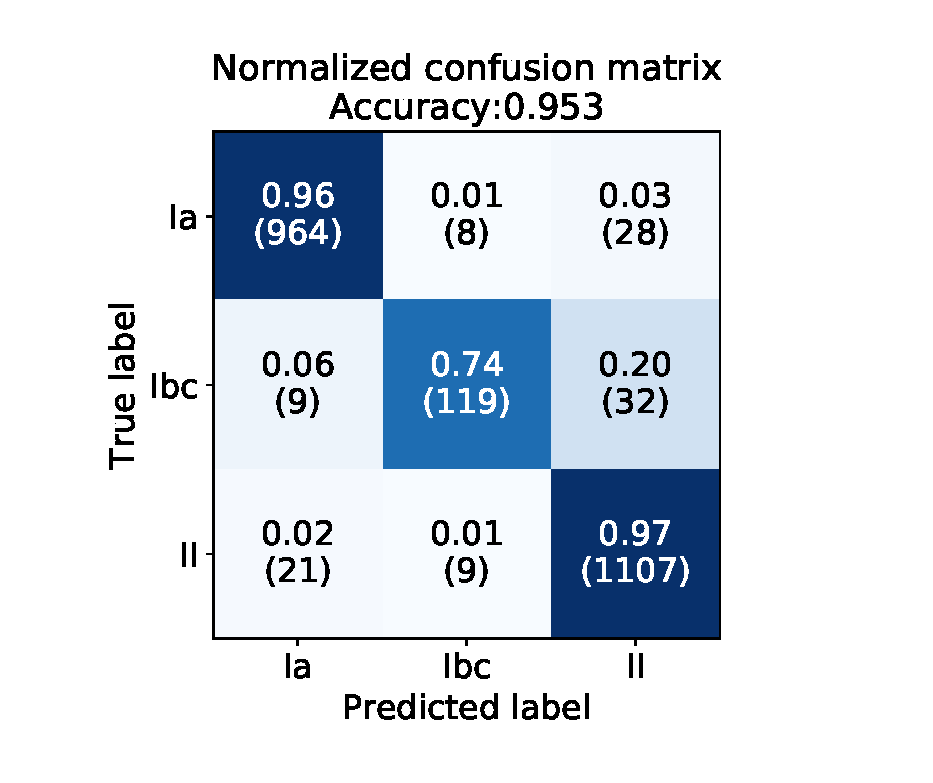
\includegraphics[width=\columnwidth]{figures/06_CM_abs-mag_scaled-flux_w-mixup_predictions_test_2.eps}
  \end{center}
  \caption{%
  Normalized confusion matrix in \DIFaddbeginFL \DIFaddFL{the }\DIFaddendFL three-class classification of \DIFaddbeginFL \DIFaddFL{the }\DIFaddendFL PLAsTiCC dataset. The \DIFdelbeginFL \DIFdelFL{input to the }\DIFdelendFL classifier \DIFdelbeginFL \DIFdelFL{is }\DIFdelendFL \DIFaddbeginFL \DIFaddFL{received the }\DIFaddendFL pseudo-absolute magnitude and normalized flux \DIFaddbeginFL \DIFaddFL{as its input}\DIFaddendFL . The proportions in each row sum to 1. The numbers in parentheses represent the raw numbers.
  }%
  \label{fig:plasticc_3class_CM}
\end{figure}
%
%added IT 200707
%SN ratio vs performance
%
Table \ref{tab:snr_vs_AUC} summarizes the classification performance for each group of \DIFaddbegin \DIFadd{the }\DIFaddend test set divided according to the maximum signal-to-noise ratio of the photometric data.
It shows that the classification performance tends to \DIFdelbegin \DIFdel{be better }\DIFdelend \DIFaddbegin \DIFadd{improve }\DIFaddend as the maximum signal-to-noise ratio increases.
\begin{table}[htbp]
\tbl{Classification performance for the maximum signal-to-noise ratio (SNR).}{
\begin{tabular}{cccc}
\noalign{\vskip 2mm}
\hline
Max. SNR & Number & \multicolumn{2}{c}{AUC\footnotemark[$*$]} \\
\hline
         &        & ROC   & Pre.-Rec. \\
\hline
$<$ 5    & 31     & 0.975 & 0.983 \\
5 -- 10  & 736    & 0.989 & 0.983 \\   
10 -- 20 & 814    & 0.999 & 0.998 \\
$>$ 20   & 716    & 0.999 & 0.999 \\
\hline
All      & 2297   & 0.996 & 0.995 \\
\hline
\end{tabular}
}\label{tab:snr_vs_AUC}
\begin{tabnote}
\footnotemark[$*$] AUC for the best performing model ($M+f$).
\end{tabnote}
\end{table}
%

%
In the three-class classification of the PLAsTiCC dataset,
107 SNe \DIFdelbegin \DIFdel{is }\DIFdelend \DIFaddbegin \DIFadd{were }\DIFaddend misclassified and have the following characteristics:
\begin{itemize}
\item 54\% (58/107) of \DIFdelbegin \DIFdel{them are 'incomplete events' that do }\DIFdelend \DIFaddbegin \DIFadd{SNe were ``incomplete events'' that did }\DIFaddend not include the \DIFdelbegin \DIFdel{SN peak phase , the }\DIFdelend \DIFaddbegin \DIFadd{peak phase of the SN (the }\DIFaddend period (observed frame) of 10 days before and 20 days after \DIFdelbegin \DIFdel{peak, }\DIFdelend \DIFaddbegin \DIFadd{the peak) }\DIFaddend in the photometric data, \DIFdelbegin \DIFdel{while they are only }\DIFdelend \DIFaddbegin \DIFadd{whereas they only constitute }\DIFaddend 38\% of all events.
\item Of the \DIFdelbegin \DIFdel{rest}\DIFdelend \DIFaddbegin \DIFadd{remaining misclassifications}\DIFaddend , 29\% (14/49) are on the boundary where the difference in probability between the correct class and the predicted class is less than 0.1.
\item \DIFdelbegin \DIFdel{More }\DIFdelend \DIFaddbegin \DIFadd{In more }\DIFaddend than half of the remaining 35 events\DIFdelbegin \DIFdel{misclassify Ibc as Ia, II}\DIFdelend \DIFaddbegin \DIFadd{, Ibc was misclassified as either Ia or II.
}\DIFaddend \end{itemize}
Figure\ \ref{fig:misclass_rate_3class} shows the accuracy against redshift for the PLAsTiCC dataset.
The accuracy for Ibc is lower than that of \DIFdelbegin \DIFdel{other classes.
It is greatly reduce }\DIFdelend \DIFaddbegin \DIFadd{the other classes; in particular,
it is greatly reduced }\DIFaddend at redshifts beyond 1.0, and also decreased at redshift z of 0.1 to 0.2.
\DIFdelbegin \DIFdel{As a result of individual check, while some }\DIFdelend \DIFaddbegin \DIFadd{Manual verification of individual misclassifications revealed that, although certain }\DIFaddend misclassified SNe are \DIFdelbegin \DIFdel{so }\DIFdelend dark and indeterminate \DIFaddbegin \DIFadd{to an extent }\DIFaddend that they are difficult to classify even with conventional methods, \DIFdelbegin \DIFdel{there are also bright SNe that are }\DIFdelend \DIFaddbegin \DIFadd{a few bright SNe were also }\DIFaddend completely misclassified.
%
\begin{figure}[htbp]
  \begin{center}
     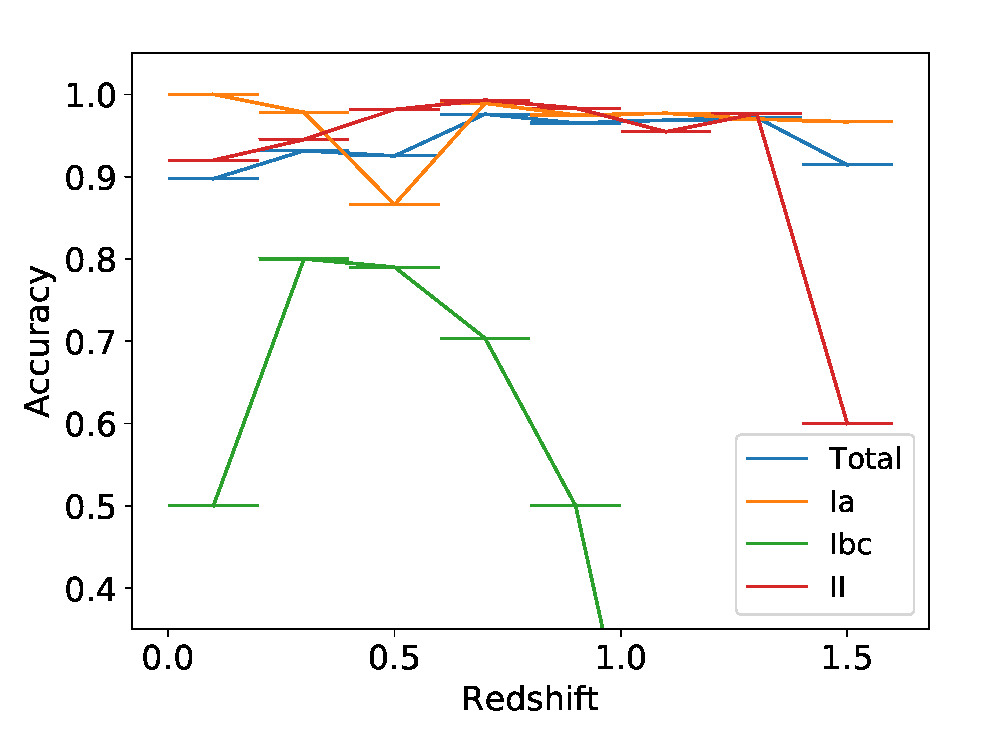
\includegraphics[width=\columnwidth]{figures/misclass_rate_plastic_3class.eps}
  \end{center}
  \caption{%
  Accuracy \DIFdelbeginFL \DIFdelFL{against }\DIFdelendFL \DIFaddbeginFL \DIFaddFL{as a function of the }\DIFaddendFL redshift in the three-class classification of the PLAsTiCC dataset.
  }%
  \label{fig:misclass_rate_3class}
\end{figure}

%%%%%%%%%%%%%%%%%%%%%%%%%%%%%%%%%%%%%%%%%%%%
%%%%%%%%%%%%%%%%%%%%%%%%%%%%%%%%%%%%%%%%%%%%
\section{Application to HSC-SSP \DIFdelbegin \DIFdel{transient survey}\DIFdelend \DIFaddbegin \DIFadd{Transient Survey}\DIFaddend }
\label{sec:h}
%
We \DIFdelbegin \DIFdel{apply }\DIFdelend \DIFaddbegin \DIFadd{applied }\DIFaddend the developed classifier to the \DIFdelbegin \DIFdel{observed photometric data set }\DIFdelend \DIFaddbegin \DIFadd{dataset acquired during the HSC-SSP Transient Survey. This dataset includes photometric data }\DIFaddend of 1824 SNe.
As described \DIFdelbegin \DIFdel{in }\DIFdelend \DIFaddbegin \DIFadd{previously }\DIFaddend \citet{yasuda19a}, the survey %is part of HSC-SSP survey, where observations were performed in two areas with different 
\DIFdelbegin \DIFdel{is }\DIFdelend \DIFaddbegin \DIFadd{was }\DIFaddend conducted in two \DIFdelbegin \DIFdel{kinds of }\DIFdelend layers with different depths and cadence, \DIFdelbegin \DIFdel{'Deep' and '}\DIFdelend \DIFaddbegin \DIFadd{i.e., ``Deep'' and ``}\DIFaddend Ultra-Deep\DIFdelbegin \DIFdel{'.}\DIFdelend \DIFaddbegin \DIFadd{.''
}\DIFaddend Therefore, the number of photometric data points of \DIFaddbegin \DIFadd{an }\DIFaddend SN in each layer could be different.
Our DNN model requires \DIFdelbegin \DIFdel{the }\DIFdelend exactly the same number of data points as \DIFdelbegin \DIFdel{an input, and here we divide our data set }\DIFdelend \DIFaddbegin \DIFadd{its input; thus, we divided our dataset }\DIFaddend into five cases based on the number of photometric data points.
%
The number of SNe for each case is summarized in table\ \ref{tab:class_flag}.
For example, the number of SNe in Case 0 is 709, and they are in the Ultra-Deep field. Each SN \DIFdelbegin \DIFdel{has }\DIFdelend \DIFaddbegin \DIFadd{is represented by }\DIFaddend a total of 
42 epochs of photometric data in four bands ($g$-, $r2$-, $i2$- and $z$-band).
The number of epochs and filter schedule for Case 0 SNe are summarized in table \ref{tab:HSCsurvey_schedule}.
\DIFdelbegin \DIFdel{By introducing five cases , the machine can }\DIFdelend \DIFaddbegin \DIFadd{The introduction of these five cases enabled the machine to correctly }\DIFaddend classify 1812 HSC SNe\DIFaddbegin \DIFadd{, }\DIFaddend which corresponds to 99.3\% of \DIFaddbegin \DIFadd{the }\DIFaddend 1824 SNe.
The remaining 12 SNe \DIFdelbegin \DIFdel{are excluded due to the }\DIFdelend \DIFaddbegin \DIFadd{were excluded owing to }\DIFaddend missing data. 
%
%v190522
\begin{table}[htbp]
\tbl{Number of SNe for each Case.}{
\begin{tabular}{lrrrr}
\noalign{\vskip 1mm}
\hline
Case & Epoch & Number & Fraction \\
\hline
0     & 42      & 709        & 0.391 \\
1     & 26      & 646        & 0.357 \\
2     & 19      & 271        & 0.150 \\
3     & 10      & 122        & 0.067 \\
4     & 4        & 64        & 0.035 \\
\hline
\end{tabular}
}\label{tab:class_flag}
\end{table}
%
%
\begin{table}[htbp]
\tbl{Number of input epochs and the schedule for Case 0 SNe.}{
\begin{tabular}{llp{15em}}
\noalign{\vskip 2mm}
\hline
Filter & Epochs & Elapsed day\\
\hline
$g$ & 8 & 2, 40, 63, 70, 92, 119, 126, 154\\
$r2$ & 9 & 5, 32, 61, 71, 92, 103, 122, 129, 151\\
$i2$ & 13 & 2, 6, 32, 40, 61, 68, 71, 94, 101, 120, 127, 154, 155\\
$z$ & 12 & 0, 6, 30, 40, 59, 68, 90, 101, 119, 126, 151, 157\\
%Y  & 10 & -59, -26, -17, 4, 13, 37, 45, 59, 68, 89 \\
\hline
\end{tabular}
}\label{tab:HSCsurvey_schedule}
\end{table}
%
%
%training set 
We \DIFdelbegin \DIFdel{apply both two-class and three-class classification to the above }\DIFdelend \DIFaddbegin \DIFadd{subjected the aforementioned }\DIFaddend five cases of \DIFdelbegin \DIFdel{HSC observed data}\DIFdelend \DIFaddbegin \DIFadd{observed HSC data to both two-class and three-class classification}\DIFaddend .
For each \DIFdelbegin \DIFdel{case}\DIFdelend \DIFaddbegin \DIFadd{of these cases}\DIFaddend , the machine needs to be trained independently with a dedicated training \DIFdelbegin \DIFdel{data set}\DIFdelend \DIFaddbegin \DIFadd{dataset}\DIFaddend .
Thus, \DIFdelbegin \DIFdel{hyperparameters are }\DIFdelend \DIFaddbegin \DIFadd{the hyperparameters were }\DIFaddend optimized for each case and \DIFaddbegin \DIFadd{are }\DIFaddend reported in table \ref{tb:searched_hp_class}.
The following subsections (subsection \ref{sec:h2} and \ref{sec:h3}) describe the performance evaluation for each classification.
%
%
\begin{table*}[t]
  \tbl{Optimized hyperparameters for classification}{
      \begin{tabular}{lcccllllllllll}
      \noalign{\vskip 1mm}
\hline
%      & $M$        & $m$        & $f$        & the number of blocks T & hidden size D & drop rate & bn & type    \\ \hline
      & \multicolumn{3}{l}{Input\footnotemark[$*$]}            & \multicolumn{5}{l}{Two-Class}      &  \multicolumn{5}{l}{Three-Class}   \\ \hline
      & $M$        & $m$        & $f$        & $T$ & $D$   & $drop\mbox{ }rate$ & $bn$ & $type$    & $T$ & $D$   & $drop\mbox{ }rate$ & $bn$ & $type$    \\ \hline      
Case 0& \checkmark &            & \checkmark & 5 & 178 & 9.47e-3   & 1  & sigmoid & 4 & 429 & 1.20e-3   & 0  & linear  \\
      & \checkmark &            &            & 3 & 247 & 9.68e-4   & 1  & sigmoid & 4 & 516 & 2.54e-3   & 0  & tanh    \\
      &            & \checkmark & \checkmark & 4 & 531 & 6.43e-3   & 0  & linear  & 4 & 608 & 1.72e-2   & 0  & linear  \\
      &            & \checkmark &            & 4 & 411 & 9.00e-2   & 1  & sigmoid & 4 & 838 & 1.36e-3   & 0  & tanh    \\ \hline
Case 1& \checkmark &            & \checkmark & 5 & 734 & 8.75e-4   & 0  & tanh    & 4 & 915 & 1.03e-2   & 0  & linear  \\
      & \checkmark &            &            & 2 & 389 & 7.17e-2   & 1  & sigmoid & 5 & 698 & 2.79e-2   & 0  & linear  \\
      &            & \checkmark & \checkmark & 2 & 647 & 7.92e-4   & 0  & tanh    & 4 & 540 & 1.45e-3   & 0  & linear  \\
      &            & \checkmark &            & 2 & 342 & 1.42e-2   & 1  & sigmoid & 2 & 520 & 9.99e-4   & 1  & sigmoid \\ \hline
Case 2& \checkmark &            & \checkmark & 2 & 368 & 1.79e-3   & 1  & sigmoid & 4 & 698 & 9.08e-4   & 0  & linear  \\
      & \checkmark &            &            & 4 & 920 & 1.44e-3   & 0  & sigmoid & 4 & 614 & 7.03e-3   & 0  & linear  \\
      &            & \checkmark & \checkmark & 5 & 572 & 4.27e-3   & 1  & sigmoid & 4 & 896 & 8.58e-3   & 0  & linear  \\
      &            & \checkmark &            & 4 & 640 & 1.12e-1   & 1  & sigmoid & 5 & 300 & 5.00e-1   & 1  & sigmoid \\ \hline
Case 3& \checkmark &            & \checkmark & 5 & 893 & 1.42e-3   & 1  & sigmoid & 4 & 522 & 5.02e-4   & 0  & tanh    \\
      & \checkmark &            &            & 4 & 880 & 1.98e-2   & 1  & sigmoid & 5 & 841 & 4.96e-2   & 1  & sigmoid \\
      &            & \checkmark & \checkmark & 3 & 300 & 5.00e-3   & 1  & linear  & 3 & 462 & 9.28e-4   & 1  & sigmoid \\
      &            & \checkmark &            & 3 & 930 & 9.77e-2   & 1  & sigmoid & 3 & 300 & 5.00e-3   & 1  & sigmoid \\ \hline
Case 4& \checkmark &            & \checkmark & 5 & 379 & 4.21e-3   & 1  & sigmoid & 3 & 484 & 2.13e-3   & 0  & linear  \\
      & \checkmark &            &            & 2 & 631 & 1.77e-2   & 0  & sigmoid & 4 & 243 & 3.21e-3   & 1  & sigmoid \\
      &            & \checkmark & \checkmark & 5 & 140 & 4.04e-3   & 1  & sigmoid & 5 & 389 & 1.23e-4   & 0  & tanh    \\
      &            & \checkmark &            & 4 & 567 & 5.77e-2   & 0  & sigmoid & 3 & 354 & 2.14e-1   & 1  & sigmoid \\ \hline
\end{tabular}
  }\label{tb:searched_hp_class}
\begin{tabnote}
\footnotemark[$*$] Input to classifier is displayed as \DIFaddbeginFL \DIFaddFL{a }\DIFaddendFL check mark. $M$: pseudo-absolute magnitude, $m$: magnitude, $f$: normalized flux.
\end{tabnote}
\end{table*}
%
%
%
%%%%%%%%%%%%%%%%%%%%%%%%%%%%%%%%%%%%%%%%%%%%%%%%%
\subsection{Binary classification}
\label{sec:h2}
%
\DIFdelbegin \DIFdel{In binary classification , we prepare }\DIFdelend \DIFaddbegin \DIFadd{Binary classification was performed using }\DIFaddend four versions of classifiers\DIFaddbegin \DIFadd{, which we prepared }\DIFaddend with different inputs as in \DIFdelbegin \DIFdel{PLAsTiCC dataset, and }\DIFdelend \DIFaddbegin \DIFadd{the PLAsTiCC dataset. This approach allowed us to }\DIFaddend compare their performance\DIFdelbegin \DIFdel{.
The performance for each input of binary classification are summarized }\DIFdelend \DIFaddbegin \DIFadd{, a summary of which is provided }\DIFaddend in table\ \ref{tab:h2_AUC}.

For the validation dataset, which is \DIFdelbegin \DIFdel{a }\DIFdelend part of the simulated dataset, a higher number of input dimensions \DIFdelbegin \DIFdel{results in the better the results, and any classifier can classify them }\DIFdelend \DIFaddbegin \DIFadd{were found to improve the results, enabling any classifier to classify the data }\DIFaddend with very high \DIFdelbegin \DIFdel{AUCs}\DIFdelend \DIFaddbegin \DIFadd{AUC}\DIFaddend .
The best AUCs for all classified events are 0.993 and 0.995 for the ROC \DIFdelbegin \DIFdel{curve }\DIFdelend and precision-recall curve, respectively.

For \DIFaddbegin \DIFadd{the }\DIFaddend test dataset, the classification performance \DIFdelbegin \DIFdel{is }\DIFdelend \DIFaddbegin \DIFadd{was }\DIFaddend verified using 1332 HSC SNe (1256 with redshift) labeled by the SALT2 \DIFdelbegin \DIFdel{light curve }\DIFdelend \DIFaddbegin \DIFadd{light-curve }\DIFaddend fitter \citep{guy2007,guy10b}, \DIFdelbegin \DIFdel{one of the conventional classification methods}\DIFdelend \DIFaddbegin \DIFadd{a conventional classification method}\DIFaddend .
The verification label for \DIFaddbegin \DIFadd{the }\DIFaddend HSC SNe conforms to \DIFaddbegin \DIFadd{that reported previously }\DIFaddend \citet{yasuda19a}, which defines SN~Ia as SNe that satisfy all \DIFdelbegin \DIFdel{the following four }\DIFdelend \DIFaddbegin \DIFadd{four of the following }\DIFaddend criteria for the SALT2 fitting results:
(1)color ($c$), and stretch ($x_1$) within the $3\sigma$ range of \citet{scolnickessler2016} \DIFdelbegin \DIFdel{'}\DIFdelend \DIFaddbegin \DIFadd{``}\DIFaddend All G10\DIFdelbegin \DIFdel{' }\DIFdelend \DIFaddbegin \DIFadd{'' }\DIFaddend distribution, 
(2)absolute magnitude in B band $M_B$ brighter than $-18.5$ mag, 
(3)reduced $\chi ^{2}$ of less than 10,
(4)number of degrees of freedom (dof) \DIFdelbegin \DIFdel{is }\DIFdelend greater than or equal to \DIFdelbegin \DIFdel{5.
}\DIFdelend \DIFaddbegin \DIFadd{five.
}\DIFaddend Other candidates that satisfy the looser set of conditions above \DIFdelbegin \DIFdel{are labeled 'Ia?'.}\DIFdelend \DIFaddbegin \DIFadd{were labeled ``Ia?.''
}\DIFaddend Specifically, the range \DIFdelbegin \DIFdel{of }\DIFdelend \DIFaddbegin \DIFadd{in }\DIFaddend (1) \DIFdelbegin \DIFdel{is }\DIFdelend \DIFaddbegin \DIFadd{was }\DIFaddend expanded to within 5 sigma, and the thresholds of (2) and (3) \DIFdelbegin \DIFdel{are }\DIFdelend \DIFaddbegin \DIFadd{were }\DIFaddend set to $-17.5$ mag and 20\DIFdelbegin \DIFdel{respectively.
On the other hand, we define non Ia }\DIFdelend \DIFaddbegin \DIFadd{, respectively.
Meanwhile, we defined non-Ia }\DIFaddend in the HSC classification as SNe that do not satisfy the conditions \DIFdelbegin \DIFdel{of 'Ia' and 'Ia?',and whose }\DIFdelend \DIFaddbegin \DIFadd{to be classified as ``Ia'' and ``Ia?,'' and of which the }\DIFaddend number of dof is \DIFdelbegin \DIFdel{5 }\DIFdelend \DIFaddbegin \DIFadd{five }\DIFaddend or more.
The \DIFdelbegin \DIFdel{numbers }\DIFdelend \DIFaddbegin \DIFadd{number }\DIFaddend of labeled Ia, Ia?\DIFdelbegin \DIFdel{and non Ia }\DIFdelend \DIFaddbegin \DIFadd{, and non-Ia }\DIFaddend are 429, 251\DIFaddbegin \DIFadd{, }\DIFaddend and 908 (410, 240\DIFaddbegin \DIFadd{, }\DIFaddend and 850, with redshift), respectively.
\DIFdelbegin \DIFdel{Besides }\DIFdelend \DIFaddbegin \DIFadd{Apart from }\DIFaddend the above, 215 SNe with \DIFdelbegin \DIFdel{the number of dof }\DIFdelend less than 5 \DIFdelbegin \DIFdel{are labeled as 'unclassified',and fitting of }\DIFdelend \DIFaddbegin \DIFadd{dof were labeled as ``unclassified,'' and }\DIFaddend the remaining 21 SNe \DIFdelbegin \DIFdel{fails.
In this performance evaluation , we use }\DIFdelend \DIFaddbegin \DIFadd{failed to be fitted.
This performance evaluation was conducted by using }\DIFaddend 428 Ia and 904 \DIFdelbegin \DIFdel{non Ia }\DIFdelend \DIFaddbegin \DIFadd{non-Ia }\DIFaddend SNe classified by our machine.

We also extracted 441 \DIFdelbegin \DIFdel{'light curve verified SNe' that have }\DIFdelend \DIFaddbegin \DIFadd{``light-curve verified SNe'' for which }\DIFaddend spec-z and photometric information \DIFaddbegin \DIFadd{were available }\DIFaddend before and after \DIFaddbegin \DIFadd{their }\DIFaddend peak, and verified their classification results.
Figures\ \ref{fig:h2_test_all} and \ref{fig:h2_test_gold} show the AUCs of the best classifier for all labeled HSC SNe and the \DIFdelbegin \DIFdel{light curve }\DIFdelend \DIFaddbegin \DIFadd{light-curve }\DIFaddend verified HSC SNe\DIFaddbegin \DIFadd{, }\DIFaddend respectively.
The confusion matrices for each case are shown in figure\ \ref{fig:h2_test_CM}.
The best performing classifier \DIFdelbegin \DIFdel{shows }\DIFdelend \DIFaddbegin \DIFadd{obtained }\DIFaddend the same classification results as the conventional method \DIFdelbegin \DIFdel{in }\DIFdelend \DIFaddbegin \DIFadd{for }\DIFaddend 84.2\% of 1256 labeled SNe, \DIFdelbegin \DIFdel{with }\DIFdelend \DIFaddbegin \DIFadd{which is }\DIFaddend 91.8\% \DIFdelbegin \DIFdel{accuracy for }\DIFdelend \DIFaddbegin \DIFadd{accurate for the }\DIFaddend 441 \DIFdelbegin \DIFdel{light curve }\DIFdelend \DIFaddbegin \DIFadd{light-curve }\DIFaddend verified SNe.
%
%
%
%2class AUC
%Ver. 1.2.0 
\begin{table*}[htbp]
\tbl{AUC of each input in the HSC binary classification.}{
\begin{tabular}{c|ccc|p{3em}p{1.8em}p{1.8em}p{1.8em}p{1.8em}p{1.8em}|p{3em}p{1.8em}p{1.8em}p{1.8em}p{1.8em}p{1.8em}}
\noalign{\vskip 1mm}
\hline
Dataset & \multicolumn{3}{c}{Input\footnotemark[$*$]} & \multicolumn{6}{|c|}{ROC} & \multicolumn{6}{c}{Precision-Recall} \\
\hline
 & $M$ & $m$ & $f$ & Case 0 & 1 & 2 & 3 & 4 & All & Case 0 & 1 & 2 & 3 & 4 & All \\
\hline
Validation &\checkmark &            & \checkmark &       1.000&       0.990 &       0.987 &       0.976 &       0.887 &        0.993 &          1.000 &          0.993 &          0.991 &          0.983 &          0.917 &           0.995 \\
& \checkmark &            &            &       0.999&       0.980 &       0.975 &       0.959 &       0.845 &        0.987 &          0.999 &          0.986 &          0.982 &          0.972 &          0.886 &           0.991 \\
&           & \checkmark & \checkmark &       0.999&       0.983 &       0.979 &       0.963 &       0.817 &        0.988 &          0.999 &          0.988 &          0.985 &          0.973 &          0.863 &           0.992 \\
&           & \checkmark &            &       0.996&       0.971 &       0.966 &       0.938 &       0.790 &        0.980 &          0.997 &          0.980 &          0.976 &          0.955 &          0.841 &           0.985 \\
\hline
Test& \checkmark &            & \checkmark &       0.975 &       0.978 &       0.931 &       0.844 &       1.000 &        0.966 &          0.931 &          0.955 &          0.773 &          0.761 &          1.000 &           0.909 \\
(Light curve verified)& \checkmark &            &            &       0.986 &       0.967 &       0.942 &       0.967 &       0.964 &        0.971 &          0.965 &          0.935 &          0.849 &          0.966 &          0.944 &           0.934 \\
&           & \checkmark & \checkmark &       0.947 &       0.926 &       0.887 &       0.756 &       1.000 &        0.923 &          0.836 &          0.860 &          0.803 &          0.632 &          1.000 &           0.820 \\
&           & \checkmark &            &       0.945 &       0.864 &       0.854 &       0.756 &       0.643 &        0.896 &          0.826 &          0.769 &          0.752 &          0.612 &          0.687 &           0.787 \\
\hline
Test& \checkmark &            & \checkmark &       0.945 &       0.922 &       0.914 &       0.863 &       0.844 &        0.925 &          0.855 &          0.840 &          0.809 &          0.788 &          0.650 &           0.832 \\
(All labeled)& \checkmark &            &            &       0.957 &       0.909 &       0.879 &       0.908 &       0.864 &        0.922 &          0.901 &          0.814 &          0.714 &          0.885 &          0.702 &           0.817 \\
&           & \checkmark & \checkmark &       0.915 &       0.889 &       0.885 &       0.718 &       0.711 &        0.885 &          0.780 &          0.778 &          0.768 &          0.543 &          0.363 &           0.749 \\
&           & \checkmark &            &       0.911 &       0.837 &       0.855 &       0.713 &       0.656 &        0.862 &          0.773 &          0.685 &          0.712 &          0.523 &          0.385 &           0.712 \\
\hline
\end{tabular}
}\label{tab:h2_AUC}
\begin{tabnote}
\footnotemark[$*$] Input to classifier is displayed as \DIFaddbeginFL \DIFaddFL{a }\DIFaddendFL check mark. $M$: pseudo-absolute magnitude, $m$: magnitude, $f$: normalized flux.
\end{tabnote}
\end{table*}
%
% all samples
%
%
\begin{figure*}[htbp]
    \begin{tabular}{cc}
        \begin{minipage}{0.5\hsize}
            \begin{center}
                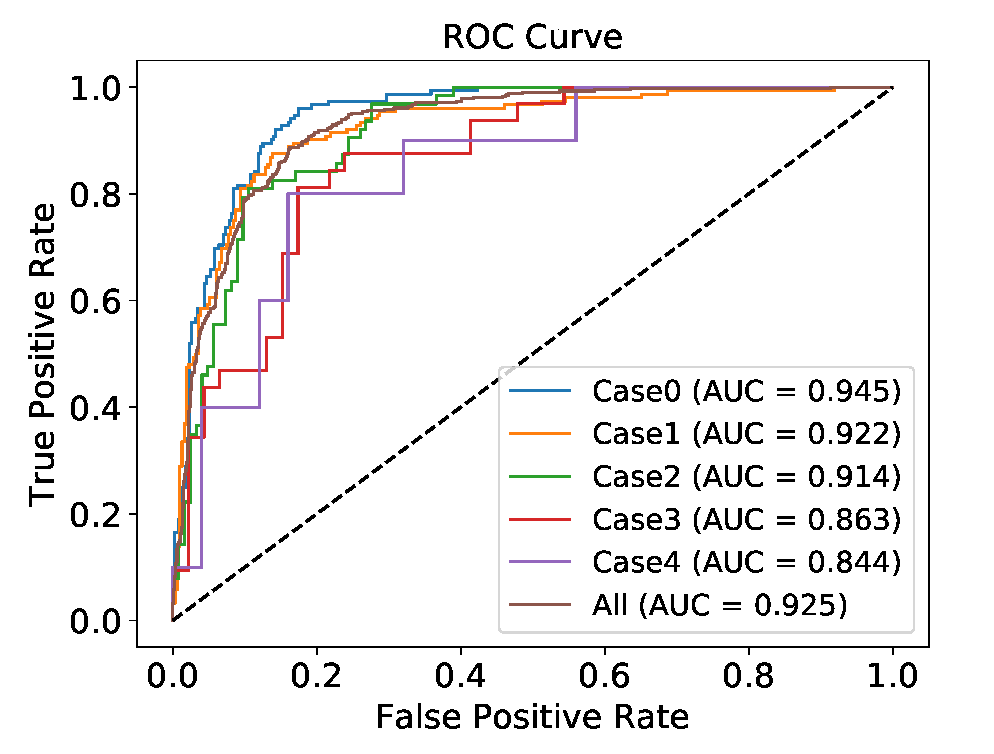
\includegraphics[width=\columnwidth]{figures/10_absolute-magnitude-scaled-flux-remove-y_SNdata_test_190522_ROC_all.eps}
            \end{center}
        \end{minipage}
        \begin{minipage}{0.5\hsize}
            \begin{center}
                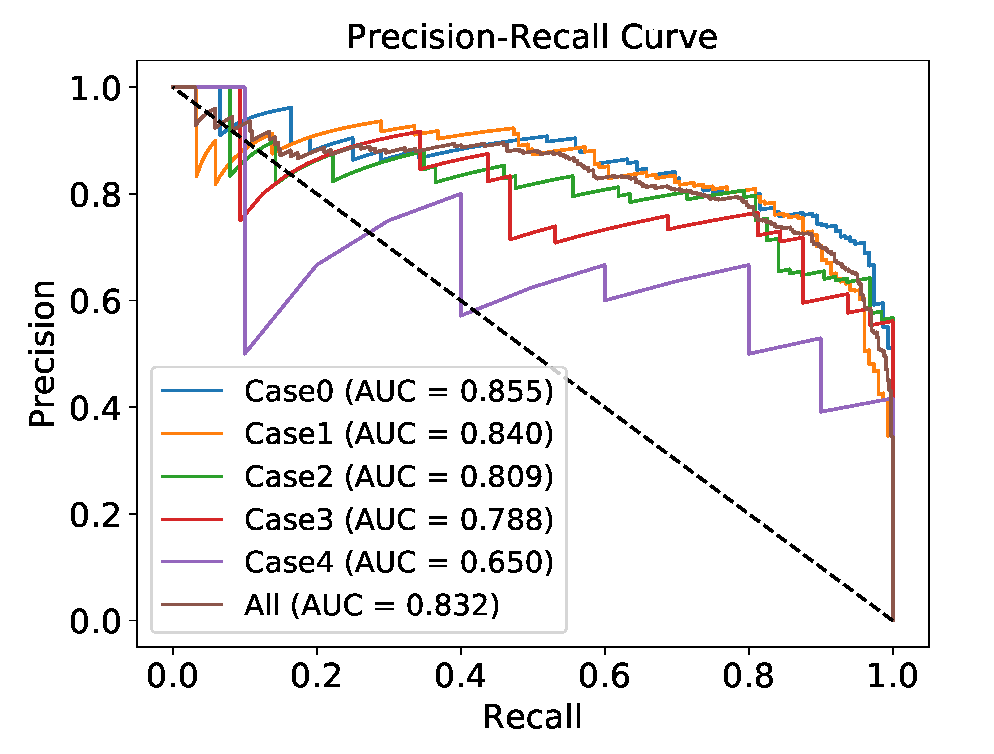
\includegraphics[width=\columnwidth]{figures/10_absolute-magnitude-scaled-flux-remove-y_SNdata_test_190522_PreRec_all.eps}
            \end{center}
        \end{minipage}
    \end{tabular}
    \vspace{2mm}
    \caption{%
    ROC curves and \DIFdelbeginFL \DIFdelFL{Precision Recall }\DIFdelendFL \DIFaddbeginFL \DIFaddFL{precision-recall }\DIFaddendFL curves \DIFdelbeginFL \DIFdelFL{in }\DIFdelendFL \DIFaddbeginFL \DIFaddFL{for the }\DIFaddendFL two-class classification of all labeled HSC SNe.
    The input to the classifier is \DIFaddbeginFL \DIFaddFL{the }\DIFaddendFL pseudo-absolute magnitude and normalized flux.
    \DIFdelbeginFL \DIFdelFL{Each }\DIFdelendFL \DIFaddbeginFL \DIFaddFL{The }\DIFaddendFL colored \DIFdelbeginFL \DIFdelFL{line represents }\DIFdelendFL \DIFaddbeginFL \DIFaddFL{lines represent }\DIFaddendFL the performance for each of the five classifiers with different input cases, and \DIFdelbeginFL \DIFdelFL{the }\DIFdelendFL that for all of their outputs.
    }
    \label{fig:h2_test_all}
\end{figure*}
%
%
%spec-z \& w/o incomplete samples
%
\begin{figure*}[htbp]
    \begin{tabular}{cc}
        \begin{minipage}{0.5\hsize}
            \begin{center}
                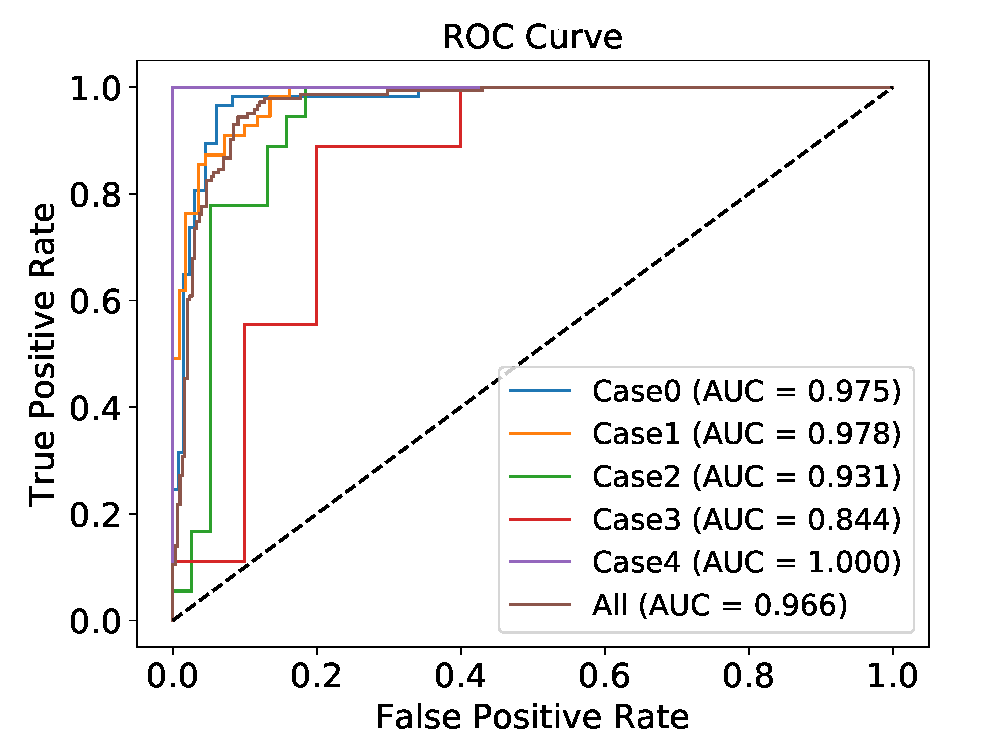
\includegraphics[width=\columnwidth]{figures/10_absolute-magnitude-scaled-flux-remove-y_SNdata_test_190522_ROC_noedge_spec.eps}
            \end{center}
        \end{minipage}
        \begin{minipage}{0.5\hsize}
            \begin{center}
                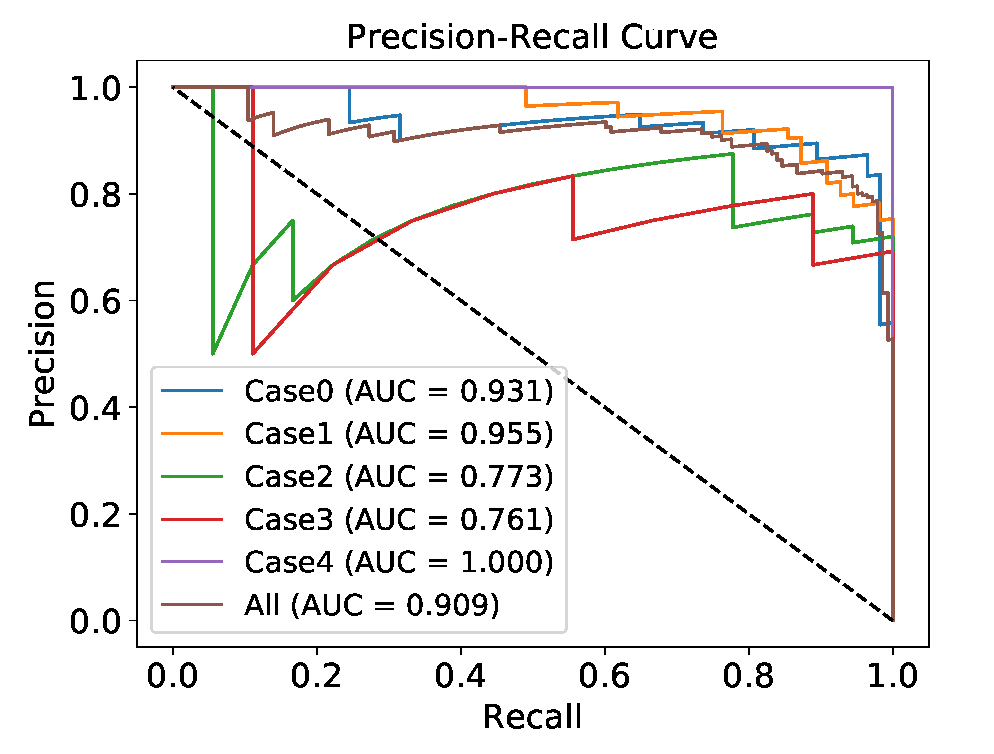
\includegraphics[width=\columnwidth]{figures/10_absolute-magnitude-scaled-flux-remove-y_SNdata_test_190522_PreRec_noedge_spec.eps}
            \end{center}
        \end{minipage}
    \end{tabular}
    \vspace{2mm}
    \caption{%
  As \DIFaddbeginFL \DIFaddFL{shown }\DIFaddendFL in figure \ref{fig:h2_test_all}, but for the \DIFdelbeginFL \DIFdelFL{light curve }\DIFdelendFL \DIFaddbeginFL \DIFaddFL{light-curve }\DIFaddendFL verified HSC SNe. 
}%
    \label{fig:h2_test_gold}
\end{figure*}
%
%
%
%
%2class Test CM
%Ver. 1.2.0
%
%% spec-z & w/o incomplete samples
%
\begin{figure*}[htbp]
    \begin{tabular}{cc}
        \begin{minipage}{0.5\hsize}
            \begin{center}
                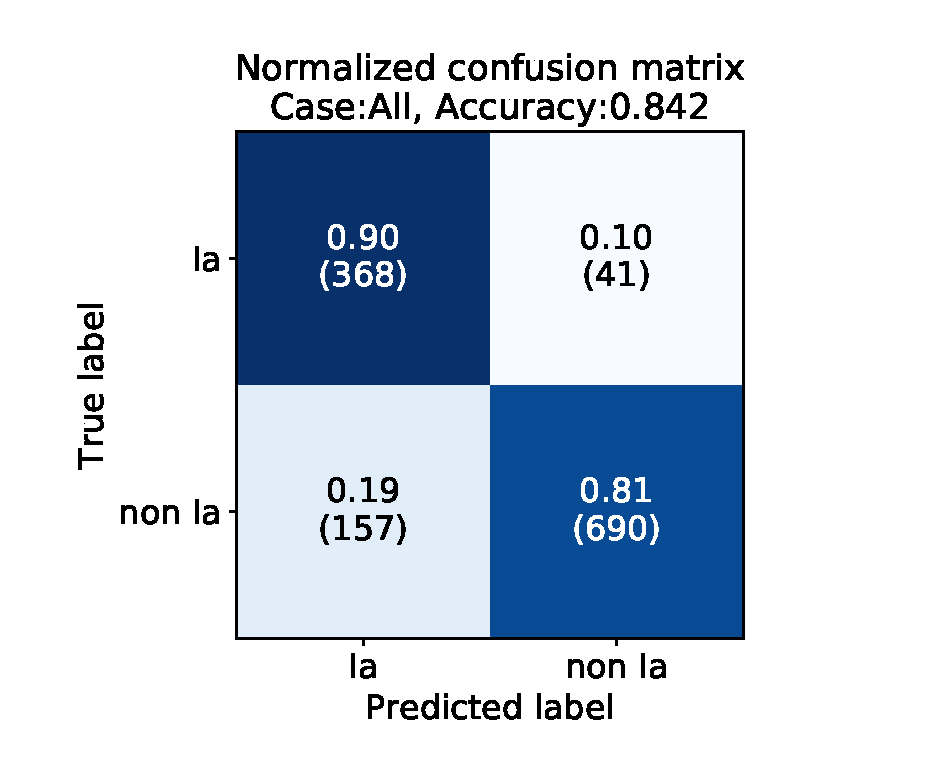
\includegraphics[width=\columnwidth]{figures/10_CM_absolute-magnitude-scaled-flux-remove-y_SNdata_test_190522_2_Flagall_all.eps}
            \end{center}
        \end{minipage}
        \begin{minipage}{0.5\hsize}
            \begin{center}
                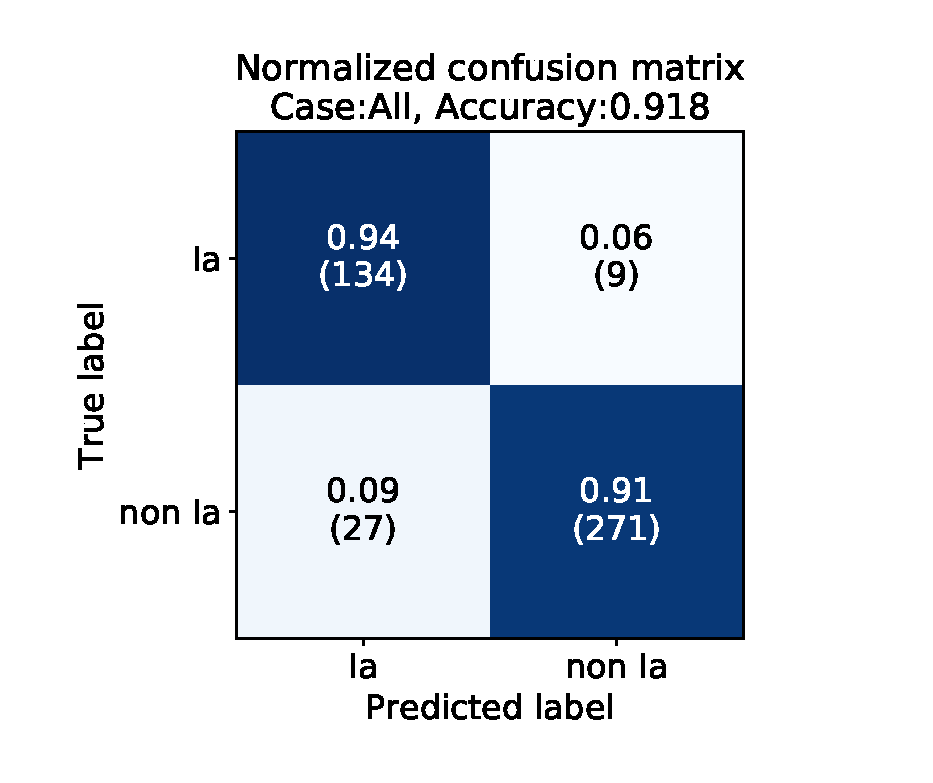
\includegraphics[width=\columnwidth]{figures/10_CM_absolute-magnitude-scaled-flux-remove-y_SNdata_test_190522_2_Flagall_noedge_spec.eps}
            \end{center}
        \end{minipage}
    \end{tabular}
    \caption{%
  Normalized confusion matrices \DIFdelbeginFL \DIFdelFL{in }\DIFdelendFL \DIFaddbeginFL \DIFaddFL{for the }\DIFaddendFL binary classification of 1256 labeled HSC SNe (left) and \DIFaddbeginFL \DIFaddFL{the }\DIFaddendFL 441 \DIFdelbeginFL \DIFdelFL{light curve }\DIFdelendFL \DIFaddbeginFL \DIFaddFL{light-curve }\DIFaddendFL verified SNe (right).
  The inputs for both classifications are \DIFaddbeginFL \DIFaddFL{the }\DIFaddendFL pseudo-absolute magnitude and normalized flux.
}%
    \label{fig:h2_test_CM}
\end{figure*}
%

In the binary classification of 1256 labeled HSC SNe, 198 of them \DIFdelbegin \DIFdel{are }\DIFdelend \DIFaddbegin \DIFadd{were }\DIFaddend misclassified.
The misclassification rate for each case is different, and tends to increase as the number of input dimensions decreases\DIFdelbegin \DIFdel{.
Although }\DIFdelend \DIFaddbegin \DIFadd{;
i.e., even though }\DIFaddend the rate is 13\% for Case 0, it is 23\% for Case 4.
As with the PLAsTiCC data, incomplete events without \DIFdelbegin \DIFdel{peak phase are }\DIFdelend \DIFaddbegin \DIFadd{their peak phase constitute }\DIFaddend the majority of misclassified events in \DIFaddbegin \DIFadd{the }\DIFaddend HSC data, accounting for 47\% (93/198) of them.
The second most common cause of misclassification is \DIFaddbegin \DIFadd{an }\DIFaddend outlier value or systematic flux offset in photometric data, accounting for 34\%(67/198) of misclassifications.
Of the remaining 38 SNe, 17 are boundary events with \DIFaddbegin \DIFadd{a }\DIFaddend Ia probability of 40 to 60\%, and the \DIFdelbegin \DIFdel{rest are events where }\DIFdelend \DIFaddbegin \DIFadd{remainder are events for which }\DIFaddend SALT2 fitting \DIFdelbegin \DIFdel{does not work well}\DIFdelend \DIFaddbegin \DIFadd{is ineffective}\DIFaddend .

%
%%%%%%%%%%%%%%%%%%%%%%%%%%%%%%%%%%%%%%%%%%%%%%%%%%%%%%%%%
%
\subsection{Multi-type classification}
\label{sec:h3}
%
In this paper, we \DIFdelbegin \DIFdel{show }\DIFdelend \DIFaddbegin \DIFadd{present }\DIFaddend the classification performance only for the validation dataset with \DIFaddbegin \DIFadd{the }\DIFaddend three-class classifier, because \DIFdelbegin \DIFdel{three type classification label is }\DIFdelend \DIFaddbegin \DIFadd{these three types of classification labels are }\DIFaddend not available for the HSC transients.
The accuracy \DIFaddbegin \DIFadd{values }\DIFaddend for each input in the three-class classification of the validation dataset are summarized in table\ \ref{tab:h3_validation}.
The best accuracy for the validation dataset is 94.0\%.
The confusion matrix of the best classifier is shown in figure \ref{fig:h3_validation_CM}.
\DIFdelbegin \DIFdel{It }\DIFdelend \DIFaddbegin \DIFadd{The result }\DIFaddend represents that our classifier has a very high sensitivity \DIFdelbegin \DIFdel{to }\DIFdelend \DIFaddbegin \DIFadd{toward }\DIFaddend SN~Ia\DIFdelbegin \DIFdel{while it is not good }\DIFdelend \DIFaddbegin \DIFadd{, whereas it is less effective }\DIFaddend at classifying SN~Ibc.

In addition, we describe the predicted classes of actual HSC SNe classified by the three-class classifier.
Figure \ref{fig:hsc3_type_frac_alongz} shows the fractions of each type predicted by the classifier in each redshift from 0.1 to 1.5.
All 1812 \DIFaddbegin \DIFadd{of the }\DIFaddend classified HSC SNe \DIFdelbegin \DIFdel{are }\DIFdelend \DIFaddbegin \DIFadd{were }\DIFaddend used to calculate the fraction.
These SN types are a combination of the outputs from the two classifiers with different inputs depending on the presence of redshift information: (1) pseudo-absolute magnitude and normalized flux, (2) magnitude and normalized flux.

%
%
%
%3class Validation
%Ver. 1.2.1
\begin{table}[htbp]
\DIFdelbeginFL %DIFDELCMD < \tbl{Accuracy of each input in the HSC three class classification for validation dataset.}{
%DIFDELCMD < \begin{tabular}{ccc|p{3em}p{1.8em}p{1.8em}p{1.8em}p{1.8em}p{1.8em}}
%DIFDELCMD < \noalign{\vskip 2mm} 
%DIFDELCMD < \hline
%DIFDELCMD < \multicolumn{3}{c}{Input\footnotemark[$*$]} & \multicolumn{6}{|c}{Accuracy\footnotemark[${\dagger}$]} \\
%DIFDELCMD < \hline
%DIFDELCMD < $M$ & $m$ & $f$  &  Case 0 & 1 & 2 & 3 & 4 &  All \\
%DIFDELCMD < \hline
%DIFDELCMD < \checkmark &            & \checkmark &        0.985 &        0.926 &        0.920 &        0.890 &        0.774 &         0.940 \\
%DIFDELCMD < \checkmark &            &            &        0.971 &        0.894 &        0.886 &        0.844 &        0.729 &         0.914 \\
%DIFDELCMD <            & \checkmark & \checkmark &        0.970 &        0.907 &        0.897 &        0.860 &        0.724 &         0.921 \\
%DIFDELCMD <            & \checkmark &            &        0.952 &        0.871 &        0.861 &        0.818 &        0.701 &         0.892 \\
%DIFDELCMD < \hline
%DIFDELCMD < \end{tabular}
%DIFDELCMD < }%%%
\DIFdelendFL \DIFaddbeginFL \tbl{Accuracy of each input in the HSC three-class classification for the validation dataset.}{
\begin{tabular}{ccc|p{3em}p{1.8em}p{1.8em}p{1.8em}p{1.8em}p{1.8em}}
\noalign{\vskip 2mm} 
\hline
\multicolumn{3}{c}{Input\footnotemark[$*$]} & \multicolumn{6}{|c}{Accuracy\footnotemark[${\dagger}$]} \\
\hline
$M$ & $m$ & $f$  &  Case 0 & 1 & 2 & 3 & 4 &  All \\
\hline
\checkmark &            & \checkmark &        0.985 &        0.926 &        0.920 &        0.890 &        0.774 &         0.940 \\
\checkmark &            &            &        0.971 &        0.894 &        0.886 &        0.844 &        0.729 &         0.914 \\
           & \checkmark & \checkmark &        0.970 &        0.907 &        0.897 &        0.860 &        0.724 &         0.921 \\
           & \checkmark &            &        0.952 &        0.871 &        0.861 &        0.818 &        0.701 &         0.892 \\
\hline
\end{tabular}
}\DIFaddendFL \label{tab:h3_validation}
\begin{tabnote}
\footnotemark[$*$] Input to classifier is displayed as \DIFaddbeginFL \DIFaddFL{a }\DIFaddendFL check mark. $M$: pseudo-absolute magnitude, $m$: magnitude, $f$: normalized flux.

\footnotemark[$\dagger$] Accuracy of samples extracted from each case according to the fractions in table \ref{tab:class_flag}.
\end{tabnote}
\end{table}
%
%
\begin{figure}[htbp]
  \begin{center}
     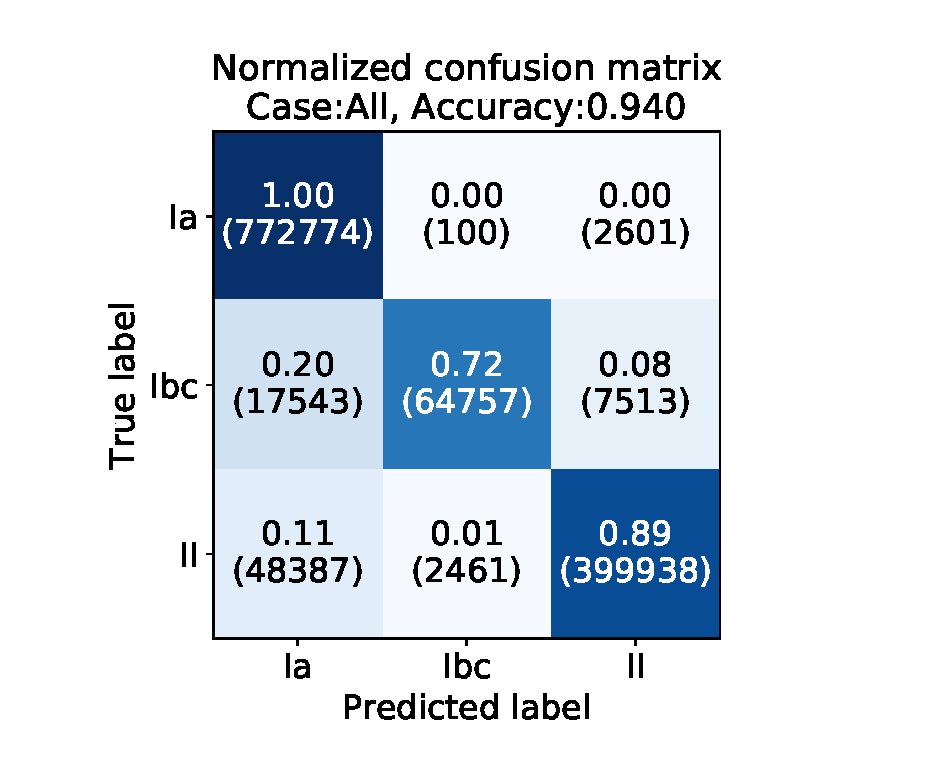
\includegraphics[width=\columnwidth]{figures/13_CM_abs-mag_scaled-flux_w-mixup_remove-y_predictions_validation_2_Flagall_weighted.eps}
  \end{center}
  \caption{%
  Normalized confusion matrix for validation dataset in the HSC three-class classification.
  The input is \DIFaddbeginFL \DIFaddFL{the }\DIFaddendFL pseudo-absolute magnitude and normalized flux.
  The proportions in each row sum to 1 (within \DIFaddbeginFL \DIFaddFL{the }\DIFaddendFL rounding error).
  }%
  \label{fig:h3_validation_CM}
\end{figure}
%
%
%
\begin{figure}[htbp]
  \begin{center}
     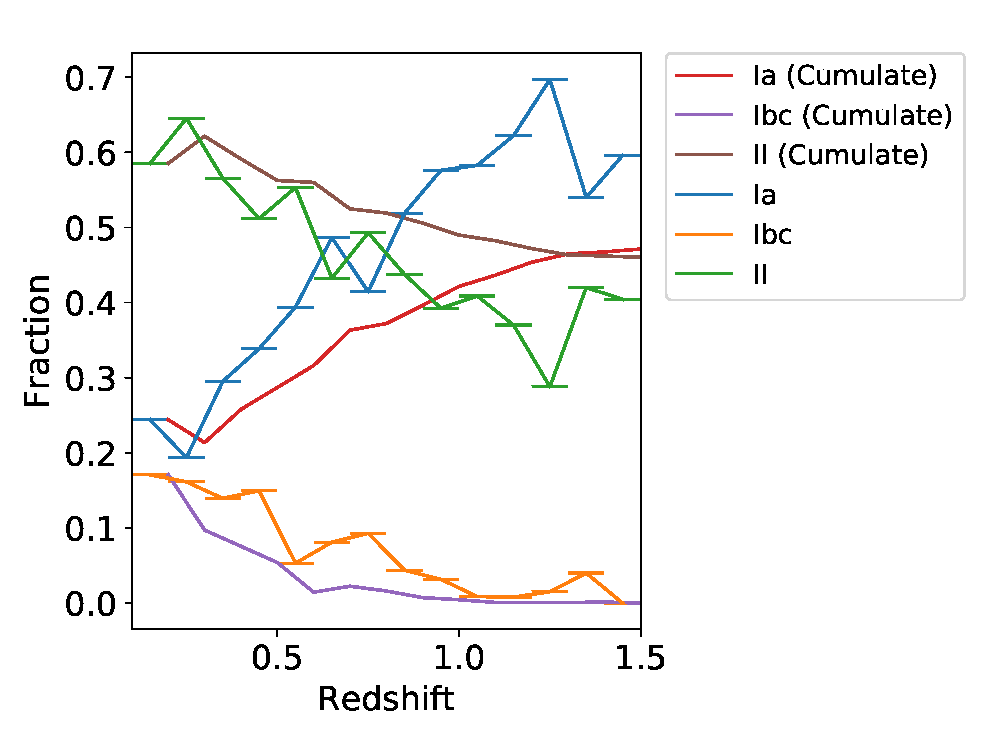
\includegraphics[width=\columnwidth]{figures/SNfrac_alongz.eps}
  \end{center}
  \caption{%
  Type fractions along redshift in HSC three-class classification.
  }%
  \label{fig:hsc3_type_frac_alongz}
\end{figure}
%

%
\subsection{Classification of HSC SNe}
%
We \DIFdelbegin \DIFdel{here publish }\DIFdelend \DIFaddbegin \DIFadd{report }\DIFaddend the classification results of 1824 HSC SNe, obtained by the proposed classifiers, in e-table 1.\footnote{ E-table 1 is available \DIFdelbegin \DIFdel{on }\DIFdelend \DIFaddbegin \DIFadd{in }\DIFaddend the online edition as a supplementary table. }
\DIFdelbegin \DIFdel{A part }\DIFdelend \DIFaddbegin \DIFadd{Part }\DIFaddend of this classification list is \DIFdelbegin \DIFdel{shown }\DIFdelend \DIFaddbegin \DIFadd{provided }\DIFaddend in table\ \ref{tab:h_results} as an example.
This list summarizes the probabilities predicted by the two-class and three-class classifiers for each SN, along with \DIFdelbegin \DIFdel{redshifts of }\DIFdelend \DIFaddbegin \DIFadd{the redshifts of the }\DIFaddend host galaxies and \DIFdelbegin \DIFdel{classification labels by }\DIFdelend \DIFaddbegin \DIFadd{the classification labels assigned on the basis of the }\DIFaddend SALT2 \DIFdelbegin \DIFdel{fit}\DIFdelend \DIFaddbegin \DIFadd{fitting}\DIFaddend .
The probabilities in this list are calculated from the output of the classifier with the normalized flux added to the input.
Each classification performance shown in subsections \ref{sec:h2} and \ref{sec:h3} is calculated based on the probabilities in this list.
\begin{table*}[htbp]
\tbl{Example of classification result list for HSC SNe.}{
%\tiny
\scriptsize
\begin{tabular}{p{4.5em}p{1.2em}p{4.0em}p{2.1em}|p{0.6em}p{1.8em}p{3.0em}|p{2.9em}|p{1.2em}p{1.2em}p{1.2em}p{0.6em}|p{2.9em}|p{1.2em}p{1.2em}p{1.2em}p{0.6em}}
\noalign{\vskip 1mm}
%\multicolumn{6}{|c}{Accuracy}
\hline
Name  &  Case &        z &  z\_src\footnotemark[$*$] &  \multicolumn{3}{p{6.0em}}{SALT2 fitting} &\multicolumn{5}{|p{13.5em}}{Classifier (Input\footnotemark[$\dagger$]: $M+f$)} & \multicolumn{5}{|p{12.0em}}{Classifier (Input\footnotemark[$\dagger$]: $m+f$)}\\
\hline
      &       &          &          &  dof & Type\footnotemark[$\ddagger$] & F\_cover\footnotemark[$\S$]  & 2-class &\multicolumn{4}{p{10.0em}|}{3-class}&2-class &    \multicolumn{4}{p{10.0em}}{3-class}\\
\hline
      &       &          &          &      &        &        &    Ia &    Ia &   Ibc &    II  &Type &   Ia &    Ia &   Ibc &    II &Type\\
\hline
HSC16aaau &     1 &    $0.370_{-0.072}^{+0.110}$ &         3 &    7 &    Ia? &   False &    0.556 &    0.554 &    0.022 &    0.424 &      Ia &    0.517 &    0.649 &    0.008 &    0.342 &      Ia \\
HSC16aaav &     1 &    $3.280_{-2.423}^{+0.167}$ &         4 &   17 &  nonIa &     True &    0.134 &    0.049 &    0.002 &    0.949 &      II &    0.279 &    0.356 &    0.048 &    0.596 &      II \\
HSC16aabj &     0 &    $0.361_{-0.008}^{+0.007}$ &         2 &    8 &  nonIa &   False &    0.630 &    0.667 &    0.001 &    0.331 &      Ia &    0.574 &    0.578 &    0.018 &    0.405 &      Ia \\
HSC16aabk &     1 &      -- &         0 &    9 &    Ia? &   False &      -- &      -- &      -- &      -- &     -- &    0.433 &    0.675 &    0.077 &    0.248 &      Ia \\
HSC16aabp &     1 &    $1.477_{-0.032}^{+0.037}$ &         2 &   19 &  nonIa &   False &    0.957 &    0.964 &    0.001 &    0.035 &      Ia &    0.807 &    0.871 &    0.039 &    0.090 &      Ia \\
\vdots & & & & & & & & & & & & & & & &\\
HSC17bjrb &     1 &    $0.560_{-0.036}^{+0.024}$ &         3 &    1 &  UC &   False &    0.003 &    0.007 &    0.004 &    0.989 &      II &    0.011 &    0.002 &    0.004 &    0.994 &      II \\
HSC17bjwo &     0 &    $1.449_{-0.063}^{+0.080}$ &         2 &   26 &     Ia &     True &    0.881 &    0.915 &    0.005 &    0.080 &      Ia &    0.891 &    0.935 &    0.010 &    0.055 &      Ia \\
HSC17bjya &     0 &    $1.128_{-0.000}^{+0.000}$ &         1 &   22 &  nonIa &     True &    0.130 &    0.145 &    0.039 &    0.816 &      II &    0.141 &    0.109 &    0.056 &    0.835 &      II \\
HSC17bjyn &     0 &    $0.626_{-0.000}^{+0.000}$ &         1 &   24 &     Ia &     True &    0.887 &    0.891 &    0.031 &    0.078 &      Ia &    0.965 &    0.918 &    0.007 &    0.075 &      Ia \\
HSC17bjza &     1 &    $1.350_{-0.156}^{+1.142}$ &         4 &   13 &  nonIa &     True &    0.016 &    0.041 &    0.016 &    0.943 &      II &    0.062 &    0.039 &    0.005 &    0.957 &      II \\
HSC17bkbn &     0 &    $0.863_{-0.012}^{+0.036}$ &         2 &   23 &  nonIa &     True &    0.031 &    0.025 &    0.002 &    0.973 &      II &    0.028 &    0.021 &    0.002 &    0.976 &      II \\
HSC17bkcz &     0 &    $0.795_{-0.000}^{+0.000}$ &         1 &   27 &     Ia &     True &    0.675 &    0.674 &    0.035 &    0.291 &      Ia &    0.661 &    0.789 &    0.019 &    0.191 &      Ia \\
HSC17bkef &     0 &    $2.940_{-0.087}^{+0.119}$ &         2 &    0 &   fail &    -- &    0.219 &    0.443 &    0.000 &    0.556 &      II &    0.950 &    0.947 &    0.010 &    0.043 &      Ia \\
HSC17bkem &     2 &    $0.609_{-0.000}^{+0.000}$ &         1 &   17 &     Ia &     True &    0.889 &    0.858 &    0.001 &    0.141 &      Ia &    0.901 &    0.863 &    0.023 &    0.114 &      Ia \\
HSC17bkfv &     0 &    $0.670_{-0.035}^{+0.035}$ &         3 &   23 &     Ia &     True &    0.915 &    0.906 &    0.016 &    0.078 &      Ia &    0.961 &    0.926 &    0.011 &    0.063 &      Ia \\
\vdots & & & & & & & & & & & & & & & &\\
HSC17dskd &     0 &    $0.630_{-0.000}^{+0.000}$ &         1 &    3 &  UC &   False &    0.889 &    0.863 &    0.087 &    0.050 &      Ia &    0.873 &    0.873 &    0.072 &    0.054 &      Ia \\
HSC17dsng &     0 &    $1.331_{-0.048}^{+0.048}$ &         2 &    7 &    Ia? &   False &    0.951 &    0.967 &    0.006 &    0.027 &      Ia &    0.935 &    0.895 &    0.011 &    0.094 &      Ia \\
HSC17dsoh &     0 &    $1.026_{-0.000}^{+0.000}$ &         1 &    2 &  UC &   False &    0.968 &    0.968 &    0.011 &    0.020 &      Ia &    0.911 &    0.923 &    0.022 &    0.055 &      Ia \\
HSC17dsox &     0 &    $1.137_{-0.034}^{+0.041}$ &         2 &    2 &  UC &   False &    0.708 &    0.794 &    0.019 &    0.186 &      Ia &    0.721 &    0.738 &    0.040 &    0.222 &      Ia \\
HSC17dspl &     0 &    $0.624_{-0.000}^{+0.000}$ &         1 &    9 &  nonIa &   False &    0.180 &    0.065 &    0.114 &    0.821 &      II &    0.049 &    0.103 &    0.100 &    0.797 &      II \\
\hline
\end{tabular}
}\label{tab:h_results}
\begin{tabnote}
\footnotemark[$*$] Code for redshift source.
1: spec-z, 2: COSMOS photo-z, 3: HSC photo-z ultra-deep, 4: HSC photo-z deep, 0: hostless.

\footnotemark[$\dagger$] $M$: pseudo-absolute magnitude, $m$: magnitude, $f$: normalized flux.

\footnotemark[$\ddagger$] SN type labeled by SALT2 fitting, UC: unclassified.

\footnotemark[$\S$] Flag indicating whether the photometric data \DIFdelbeginFL \DIFdelFL{covers }\DIFdelendFL \DIFaddbeginFL \DIFaddFL{cover }\DIFaddendFL the period of 10 days before and 20 days after the peak. SNe with this flag set to False are defined as \DIFdelbeginFL \DIFdelFL{'incomplete events'.}\DIFdelendFL \DIFaddbeginFL \DIFaddFL{``incomplete events.''
}\DIFaddendFL \end{tabnote}
\end{table*}
%
%
\subsection{Dependence on the number of epochs}
%
When using our classification method, the number of photometric data points given to the classifier increases as the survey progresses.
Therefore, we \DIFdelbegin \DIFdel{investigate }\DIFdelend \DIFaddbegin \DIFadd{investigated }\DIFaddend the transition of performance against the number of epochs.
\DIFdelbegin \DIFdel{We classify }\DIFdelend \DIFaddbegin \DIFadd{This was accomplished by classifying }\DIFaddend the HSC dataset by increasing the number of input data points \DIFdelbegin \DIFdel{one by one, and examine }\DIFdelend \DIFaddbegin \DIFadd{in increments of one, and by examining }\DIFaddend the relationship between the number of epochs and the classification performance.
Binary classifiers \DIFdelbegin \DIFdel{are }\DIFdelend \DIFaddbegin \DIFadd{were }\DIFaddend adopted for classification, and the accuracy calculated from each confusion matrix \DIFdelbegin \DIFdel{is }\DIFdelend \DIFaddbegin \DIFadd{was }\DIFaddend used for evaluation.
Figure\ \ref{fig:n_observations} shows the transition of classification performance for the Case 0 HSC dataset along with the number of epochs.
Although the Ia accuracy is as low as 0.6 to 0.7 in the early stage of the survey with less than five epochs, it exceeds 0.8 when the number of epochs increases to 22.
The partial decrease in accuracy is thought to be due to \DIFdelbegin \DIFdel{the new SN found at the added }\DIFdelend \DIFaddbegin \DIFadd{a new SN being found upon the addition of a }\DIFaddend photometric point.
%
\begin{figure}[htbp]
  \begin{center}
     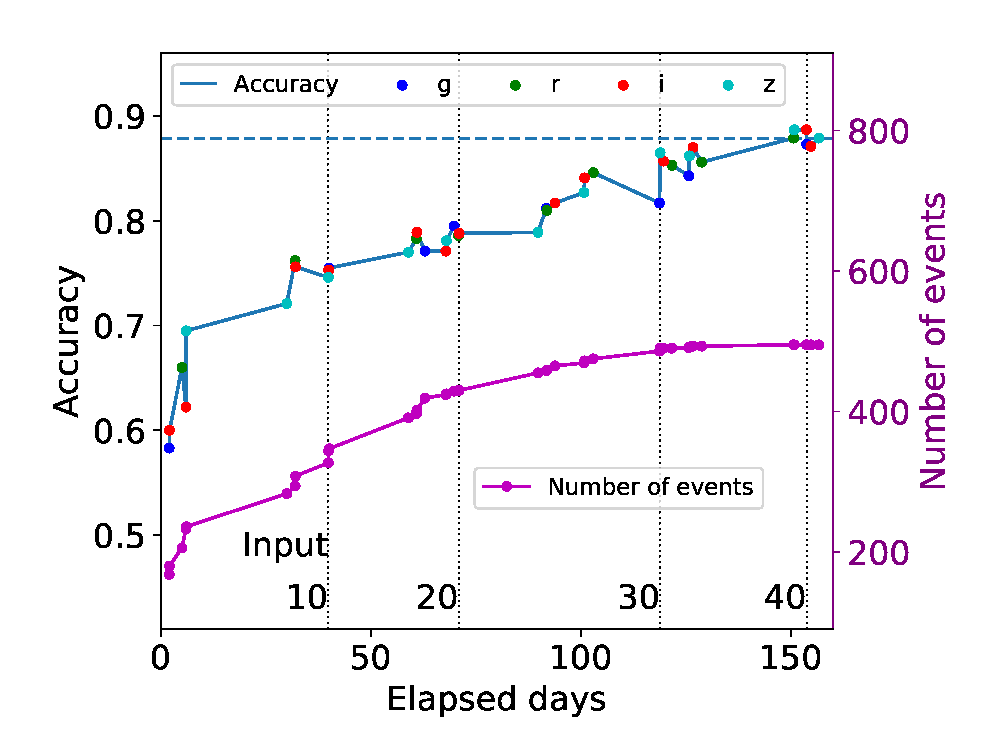
\includegraphics[width=\columnwidth]{figures/n_observations_v2_case0.eps}
  \end{center}
  \caption{%
  Relationship between the number of epochs and classification performance in binary classification for the Case 0 dataset. 
  The horizontal axis \DIFdelbeginFL \DIFdelFL{is }\DIFdelendFL \DIFaddbeginFL \DIFaddFL{represents }\DIFaddendFL the \DIFaddbeginFL \DIFaddFL{number of }\DIFaddendFL elapsed days of the HSC survey, and the vertical \DIFdelbeginFL \DIFdelFL{dot }\DIFdelendFL \DIFaddbeginFL \DIFaddFL{dotted }\DIFaddendFL line \DIFdelbeginFL \DIFdelFL{shows }\DIFdelendFL \DIFaddbeginFL \DIFaddFL{indicates }\DIFaddendFL the scale of \DIFdelbeginFL \DIFdelFL{input photometric point }\DIFdelendFL \DIFaddbeginFL \DIFaddFL{the }\DIFaddendFL number \DIFaddbeginFL \DIFaddFL{of photometric points that were used as input}\DIFaddendFL . 
  The color of each mark in accuracy indicates the band of the added photometric point. 
  The blue horizontal dotted line indicates the accuracy when using all epochs.
  }%
  \label{fig:n_observations}
\end{figure}
%

We also investigated the classification performance during each SN phase by regrouping all events according to the length of \DIFdelbegin \DIFdel{period }\DIFdelend \DIFaddbegin \DIFadd{time }\DIFaddend since the first detection.
Figure\ \ref{fig:lcps} illustrates the light curves and Ia probability transitions since the first detection of \DIFdelbegin \DIFdel{three }\DIFdelend \DIFaddbegin \DIFadd{the three types of }\DIFaddend HSC SNe.
We define \DIFdelbegin \DIFdel{'first detection' }\DIFdelend \DIFaddbegin \DIFadd{``first detection'' }\DIFaddend as the first day when the SN is detected with 5$\sigma$ confidence in flux, and \DIFaddbegin \DIFadd{which is }\DIFaddend flagged as a real object by the real-bogus classifier using \DIFaddbegin \DIFadd{a }\DIFaddend convolutional neural network \citep{yasuda19a}.
The probability is updated at each new epoch.
\DIFdelbegin \DIFdel{While there are events where }\DIFdelend \DIFaddbegin \DIFadd{Although }\DIFaddend the probability increases \DIFaddbegin \DIFadd{for certain events }\DIFaddend as the SN phase progresses, \DIFdelbegin \DIFdel{there are also some events where }\DIFdelend \DIFaddbegin \DIFadd{in the case of other events }\DIFaddend the probabilities fluctuate around 0.5 even as the observation progresses and \DIFaddbegin \DIFadd{these events }\DIFaddend cannot be clearly classified.
Figure\ \ref{fig:n_observations_SNphase} shows the relationship between the number of days \DIFdelbegin \DIFdel{from first detection to classification, accuracy }\DIFdelend \DIFaddbegin \DIFadd{since the first detection until classification, the accuracy, }\DIFaddend and the cumulative number of SNe classified as Ia with high probability.
The calculations for each performance are based on the classification results for 1161 SNe \DIFaddbegin \DIFadd{that were }\DIFaddend detected before the rising phase.
This figure presents \DIFdelbegin \DIFdel{how long }\DIFdelend \DIFaddbegin \DIFadd{the time span of }\DIFaddend SN photometric data \DIFdelbegin \DIFdel{is needed to classify with high accuracy }\DIFdelend \DIFaddbegin \DIFadd{that is needed for highly accurate classification }\DIFaddend using our classifier.
The classification accuracy is 78.1\% for the first two weeks of data, and after one month it increases to 82.7\%.
In addition, the number of follow-up candidates \DIFaddbegin \DIFadd{identified }\DIFaddend by the classifier can be estimated from the cumulative number in figure \ref{fig:n_observations_SNphase}.
Using data \DIFaddbegin \DIFadd{acquired }\DIFaddend within one month from the first detection, 79 SNe with z $>$ 1 \DIFdelbegin \DIFdel{are }\DIFdelend \DIFaddbegin \DIFadd{could be }\DIFaddend classified with Ia probability of 95\% or more.
\DIFdelbegin \DIFdel{Since }\DIFdelend \DIFaddbegin \DIFadd{Because }\DIFaddend the number of these SNe is a cumulative number \DIFdelbegin \DIFdel{for six monthsobservation}\DIFdelend \DIFaddbegin \DIFadd{observed during a period of six months}\DIFaddend , dividing this by six corresponds to the number of follow-up SNe classified during a one-month survey, which is 13 events.
%
\begin{figure*}[htbp]
    \begin{tabular}{ccc}
        \begin{minipage}{0.33\hsize}
            \begin{center}
                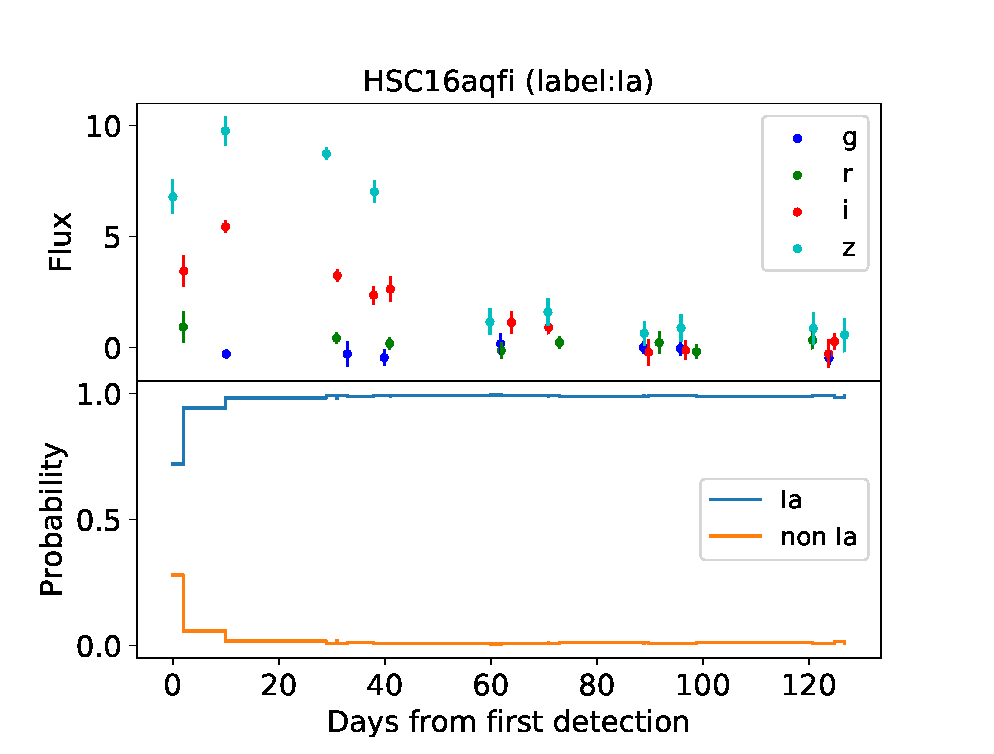
\includegraphics[width=\columnwidth]{figures/lcp_aqfi.eps}
            \end{center}
        \end{minipage}
        \begin{minipage}{0.33\hsize}
            \begin{center}
                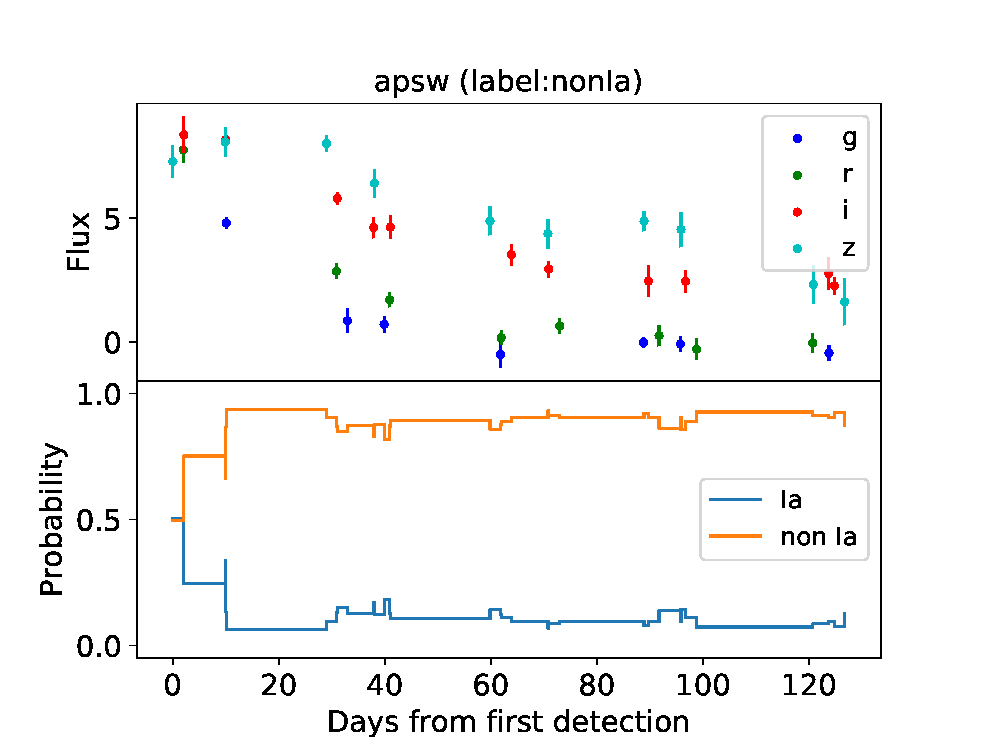
\includegraphics[width=\columnwidth]{figures/lcp_apsw.eps}
            \end{center}
        \end{minipage}
        \begin{minipage}{0.33\hsize}
            \begin{center}
                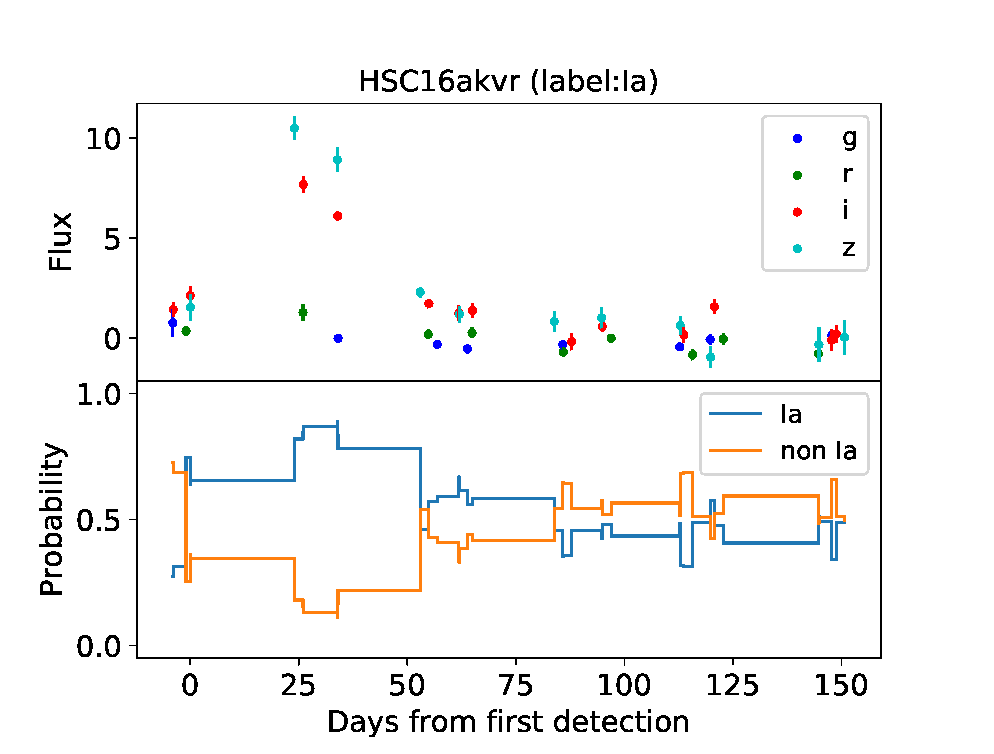
\includegraphics[width=\columnwidth]{figures/lcp_akvr.eps}
            \end{center}
        \end{minipage}
    \end{tabular}
    \vspace{3mm}
    \caption{%
    Examples of light curves and probability transitions. The title of each plot shows the name of the SN in the HSC survey and the label classified by SALT2 fitting.
    }%      
    \label{fig:lcps}
\end{figure*}
%
\begin{figure}[htbp]
  \begin{center}
     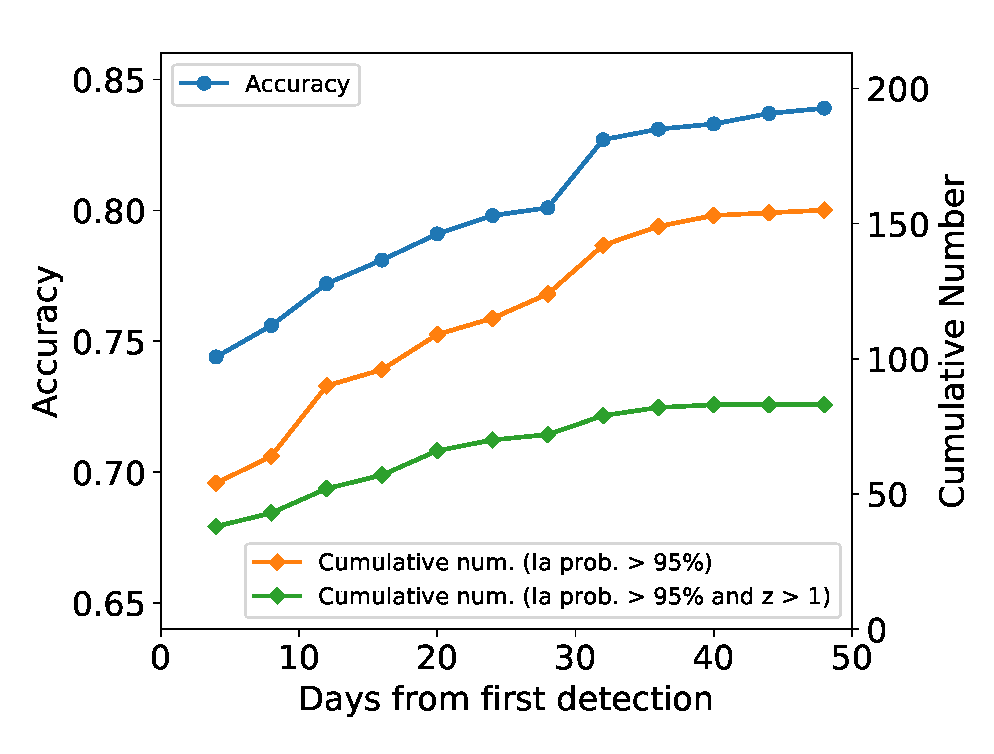
\includegraphics[width=\columnwidth]{figures/n_observations_SNphase_v200318.eps}
  \end{center}
  \caption{%
  Classification accuracy and cumulative number of \DIFdelbeginFL \DIFdelFL{type }\DIFdelendFL \DIFaddbeginFL \DIFaddFL{Type }\DIFaddendFL Ia SNe classified with high probability against \DIFaddbeginFL \DIFaddFL{the }\DIFaddendFL SN phase.
  The orange line indicates the cumulative number of SNe with Ia probability $>$ 95\%, and \DIFaddbeginFL \DIFaddFL{the }\DIFaddendFL green line is that for distant SNe at z $>$ 1.
  }%
  \label{fig:n_observations_SNphase}
\end{figure}
%

Lastly, we \DIFdelbegin \DIFdel{study }\DIFdelend \DIFaddbegin \DIFadd{studied }\DIFaddend the transition of the Ia probability output by the classifier along \DIFaddbegin \DIFadd{the }\DIFaddend SN phase.
Each time the number of input epochs increases, \DIFaddbegin \DIFadd{the }\DIFaddend Ia probability, \DIFaddbegin \DIFadd{i.e., }\DIFaddend the output of the classifier, is updated.
In Figure \ref{fig:visualized_Ia_prob} (Upper panel), we \DIFdelbegin \DIFdel{plot a }\DIFdelend \DIFaddbegin \DIFadd{plotted the }\DIFaddend Ia probability at each epoch for \DIFdelbegin \DIFdel{300 each of }\DIFdelend \DIFaddbegin \DIFadd{each of 300 }\DIFaddend SNe labeled Ia and \DIFdelbegin \DIFdel{non Ia with }\DIFdelend \DIFaddbegin \DIFadd{non-Ia based on the }\DIFaddend SALT2 fitting. \DIFdelbegin \DIFdel{By using this result , we }\DIFdelend \DIFaddbegin \DIFadd{The use of this result enabled us to }\DIFaddend measure the last epoch \DIFdelbegin \DIFdel{to classify }\DIFdelend \DIFaddbegin \DIFadd{at which }\DIFaddend the correct type \DIFaddbegin \DIFadd{is classified}\DIFaddend , i.e., the epoch after which no further change in the classification occurs, for each SN. The lower panel shows the cumulative ratio for the epoch. The figure shows that \DIFdelbegin \DIFdel{classification performance gets better with time , and about }\DIFdelend \DIFaddbegin \DIFadd{the classification performance improves with time and that approximately }\DIFaddend 80\% of supernovae are correctly classified \DIFdelbegin \DIFdel{around }\DIFdelend \DIFaddbegin \DIFadd{approximately }\DIFaddend 30 days after \DIFdelbegin \DIFdel{the }\DIFdelend \DIFaddbegin \DIFadd{their }\DIFaddend first detection. In this figure, the initial cumulative ratio is lower than the accuracy shown in Figure \ref{fig:n_observations_SNphase} because \DIFdelbegin \DIFdel{some }\DIFdelend \DIFaddbegin \DIFadd{certain }\DIFaddend SNe that are \DIFdelbegin \DIFdel{correctly classified at the beginning can finally switch to the }\DIFdelend \DIFaddbegin \DIFadd{initially correctly classified could ultimately be misclassified as the }\DIFaddend wrong type.

%
Figure \ref{fig:HSTIaprob} shows the transitions of Ia probability \DIFdelbegin \DIFdel{along the }\DIFdelend \DIFaddbegin \DIFadd{as a function of the number of }\DIFaddend days from the peak for 26 SNe selected as HST targets in the HSC survey, and the average of these transitions.
The Ia probability for the average of the candidates is greater than 0.8 three weeks before the peak.
This means that our classifier accomplishes the task described in subsection \ref{sec:tasks} \DIFdelbegin \DIFdel{to find good candidates only with information }\DIFdelend \DIFaddbegin \DIFadd{by identifying good candidate SNe even when it only has information acquired }\DIFaddend before the SN peak.
%
\begin{figure}[htbp]
  \begin{center}
     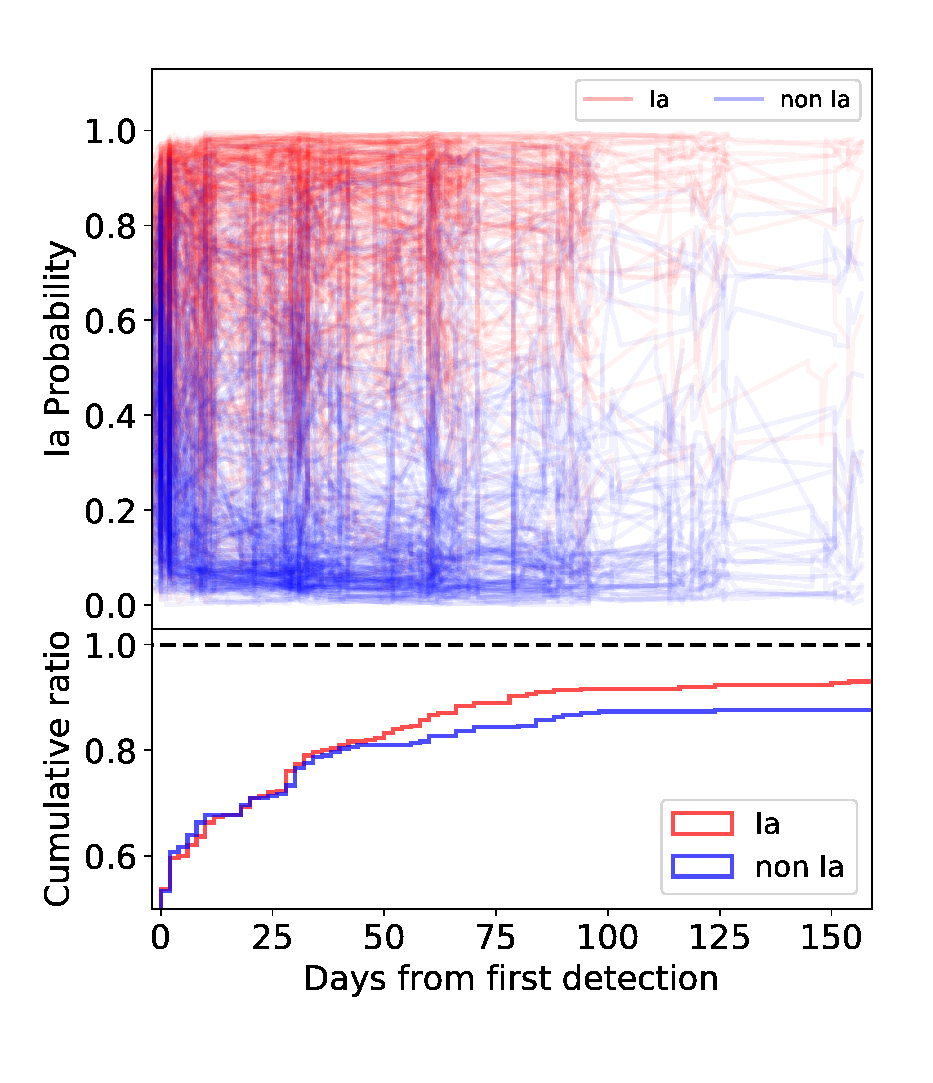
\includegraphics[width=\columnwidth]{figures/n_observations_lastestday_200709.eps}
  \end{center}
  \caption{%
  Upper panel: Transition of Ia probability of SNe after first detection. Each line corresponds to one of \DIFaddbeginFL \DIFaddFL{the }\DIFaddendFL SNe. \DIFdelbeginFL \DIFdelFL{The difference in color indicates the difference in label}\DIFdelendFL \DIFaddbeginFL \DIFaddFL{Different colors indicate different labels}\DIFaddendFL , with red being Ia and blue being \DIFdelbeginFL \DIFdelFL{non Ia}\DIFdelendFL \DIFaddbeginFL \DIFaddFL{non-Ia}\DIFaddendFL . Lower panel: Cumulative ratio for the epoch at which SNe are finally correctly classified.
  }%
  \label{fig:visualized_Ia_prob}
\end{figure}
%
%
\begin{figure}[htbp]
  \begin{center}
     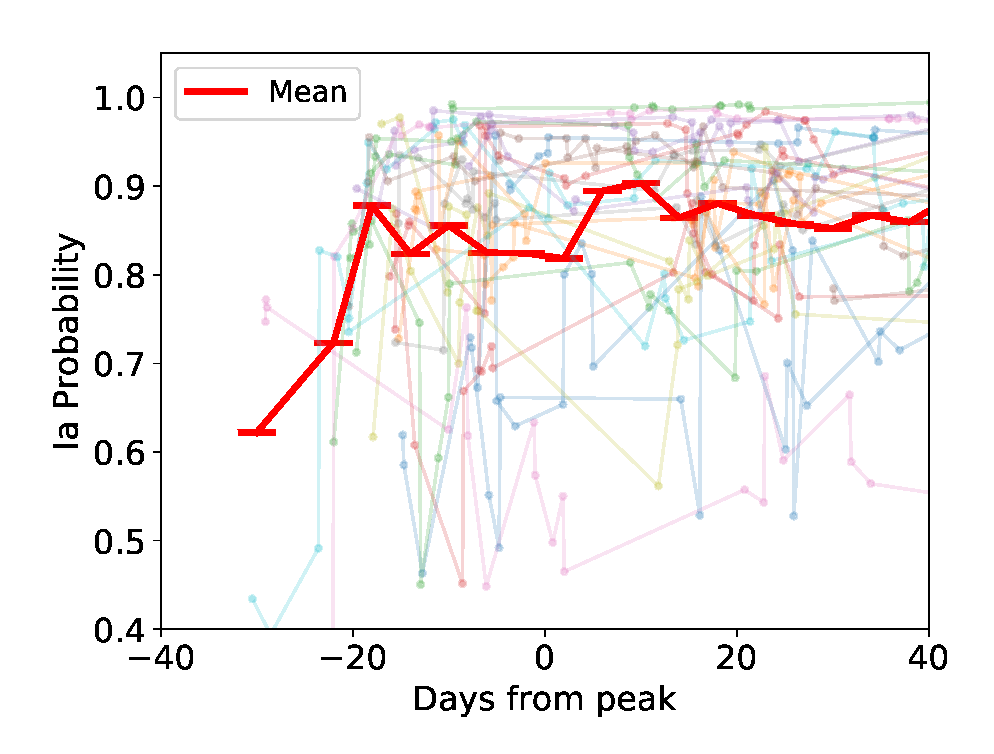
\includegraphics[width=\columnwidth]{figures/HST_DaysFromPeak_vs_IaProbability_200319.eps}
  \end{center}
  \caption{%
  Ia probability transitions of 26 HST targets. Each of the lighter lines represents the variation for \DIFdelbeginFL \DIFdelFL{the }\DIFdelendFL individual HST targets, and the red line is \DIFdelbeginFL \DIFdelFL{those }\DIFdelendFL \DIFaddbeginFL \DIFaddFL{the }\DIFaddendFL average \DIFaddbeginFL \DIFaddFL{of these lines}\DIFaddendFL .
  }%
  \label{fig:HSTIaprob}
\end{figure}
%
%
%%%%%%%%%%%%%%%%%%%%%%%%%%%%%%%%%%%%%%%%%%%%%%%%%%%%
\section{Discussion}
%
\subsection{Factors affecting classifier performance}
%
In this \DIFdelbegin \DIFdel{paper, we apply }\DIFdelend \DIFaddbegin \DIFadd{study, we applied }\DIFaddend our classifier to actual HSC survey data to evaluate its classification performance.
\DIFdelbegin \DIFdel{What we find out by }\DIFdelend \DIFaddbegin \DIFadd{By }\DIFaddend classifying actual data with our method\DIFdelbegin \DIFdel{is }\DIFdelend \DIFaddbegin \DIFadd{, we determined }\DIFaddend that the performance difference between the validation and test \DIFdelbegin \DIFdel{set }\DIFdelend \DIFaddbegin \DIFadd{sets }\DIFaddend is larger than that for the PLAsTiCC data.
\DIFdelbegin \DIFdel{We }\DIFdelend \DIFaddbegin \DIFadd{Here we }\DIFaddend discuss the factors that affect the classification performance of actual data.

One possible \DIFdelbegin \DIFdel{reason }\DIFdelend \DIFaddbegin \DIFadd{factor }\DIFaddend is the uncertainty in the labeling of actual data using conventional methods.
In the confusion matrix for all labeled SNe in figure \ref{fig:h2_test_CM}, 47\% of the 198 misclassified SNe are incomplete events \DIFdelbegin \DIFdel{.
They are only }\DIFdelend \DIFaddbegin \DIFadd{and these events only form }\DIFaddend 35\% of \DIFaddbegin \DIFadd{the }\DIFaddend 1824 HSC SNe.
The high percentage of incomplete events among \DIFaddbegin \DIFadd{the }\DIFaddend misclassified events suggests that \DIFdelbegin \DIFdel{they reduce }\DIFdelend \DIFaddbegin \DIFadd{incomplete events reduce the }\DIFaddend classification performance.
However, the misclassification rate of incomplete events is clearly \DIFdelbegin \DIFdel{increased to }\DIFdelend \DIFaddbegin \DIFadd{higher at }\DIFaddend 28\% (93/338) \DIFdelbegin \DIFdel{in }\DIFdelend \DIFaddbegin \DIFadd{for the }\DIFaddend HSC data compared to 7\% (58/871) \DIFdelbegin \DIFdel{in }\DIFdelend \DIFaddbegin \DIFadd{for }\DIFaddend PLAsTiCC data.
\DIFaddbegin \DIFadd{In addition, }\DIFaddend SALT2 fitting is \DIFdelbegin \DIFdel{also not good }\DIFdelend \DIFaddbegin \DIFadd{equally ineffective }\DIFaddend at fitting incomplete events \DIFdelbegin \DIFdel{due }\DIFdelend \DIFaddbegin \DIFadd{owing }\DIFaddend to its specification, and errors in \DIFaddbegin \DIFadd{the }\DIFaddend fitting parameters are significantly larger.
These \DIFdelbegin \DIFdel{facts suggests the existence }\DIFdelend \DIFaddbegin \DIFadd{findings suggest a degree }\DIFaddend of uncertainty in labeling with conventional classification methods.
Another source of uncertainty in labeling is \DIFdelbegin \DIFdel{due to the uncertainty of }\DIFdelend \DIFaddbegin \DIFadd{the uncertainty in the }\DIFaddend redshift information used in SALT2 fitting.
For at least 16 misclassified events that \DIFdelbegin \DIFdel{have no }\DIFdelend \DIFaddbegin \DIFadd{were not affected by any }\DIFaddend other misclassification factors, the fitting color parameters are far outside the criteria for Ia, and the wrong redshift \DIFdelbegin \DIFdel{is }\DIFdelend \DIFaddbegin \DIFadd{was }\DIFaddend probably used for fitting.
In fact, as shown in the \DIFdelbegin \DIFdel{right panel of }\DIFdelend \DIFaddbegin \DIFadd{panel on the right in }\DIFaddend figure \ref{fig:h2_test_CM}, the performance for \DIFdelbegin \DIFdel{light curve }\DIFdelend \DIFaddbegin \DIFadd{light-curve }\DIFaddend verified SNe, except for incomplete events and \DIFdelbegin \DIFdel{whose }\DIFdelend \DIFaddbegin \DIFadd{for events of which }\DIFaddend spec-z is known, is \DIFdelbegin \DIFdel{better than for }\DIFdelend \DIFaddbegin \DIFadd{superior to that of }\DIFaddend all classified events.

Another \DIFdelbegin \DIFdel{cause of }\DIFdelend \DIFaddbegin \DIFadd{reason for }\DIFaddend the large difference in the performance of the validation and test set is the inability to completely simulate the observed data.
Outlier values and systematic flux offsets, which are considered to be one of the causes of misclassification \DIFaddbegin \DIFadd{as }\DIFaddend described in subsection \ref{sec:h2}, are found only in \DIFaddbegin \DIFadd{real }\DIFaddend observed data.
As described \DIFdelbegin \DIFdel{in }\DIFdelend \DIFaddbegin \DIFadd{previously }\DIFaddend \citet{yasuda19a}, the photometric data of the \DIFdelbegin \DIFdel{SN }\DIFdelend \DIFaddbegin \DIFadd{SNe }\DIFaddend in the HSC survey \DIFdelbegin \DIFdel{is }\DIFdelend \DIFaddbegin \DIFadd{are }\DIFaddend measured from the difference image obtained by subtracting the reference image from the observed image.
We believe that the unsimulated residual in this subtraction \DIFdelbegin \DIFdel{creates }\DIFdelend \DIFaddbegin \DIFadd{created }\DIFaddend a difference between the photometric data \DIFaddbegin \DIFadd{that were used }\DIFaddend for training and observation, and increases the misclassification rate of the classifier \DIFdelbegin \DIFdel{in the }\DIFdelend \DIFaddbegin \DIFadd{when processing }\DIFaddend actual data.
For example, \DIFdelbegin \DIFdel{The }\DIFdelend \DIFaddbegin \DIFadd{the }\DIFaddend light curve of SN HSC16akvr shown in the \DIFdelbegin \DIFdel{right panel of }\DIFdelend \DIFaddbegin \DIFadd{panel on the right in }\DIFaddend figure \ref{fig:lcps} fluctuates at its tail\DIFdelbegin \DIFdel{part, and the }\DIFdelend \DIFaddbegin \DIFadd{, and in this part of the curve the }\DIFaddend classification is not clear\DIFdelbegin \DIFdel{in that part.
It will be necessary to reduce or simulate }\DIFdelend \DIFaddbegin \DIFadd{.
Improving the performance of the classifier would therefore necessitate the reduction or simulation of }\DIFaddend these outlier values as much as possible\DIFdelbegin \DIFdel{to improve the performance of the classifier}\DIFdelend .
%
%
%
\subsection{Comparison with other classifiers}
\label{sec:comparison}
%
\DIFdelbegin \DIFdel{When comparing }\DIFdelend \DIFaddbegin \DIFadd{The direct comparison of }\DIFaddend the classification results of the classifiers \DIFdelbegin \DIFdel{, it is difficult to make a direct comparison if there are }\DIFdelend \DIFaddbegin \DIFadd{is complicated by }\DIFaddend differences in methods, training datasets, or \DIFaddbegin \DIFadd{the }\DIFaddend number of inputs and outputs. 
Here, we simply compare the \DIFaddbegin \DIFadd{results obtained with the }\DIFaddend recent SN type classifier based on machine learning and our classifier with AUC of ROC in \DIFdelbegin \DIFdel{the binary classification of Ia or not}\DIFdelend \DIFaddbegin \DIFadd{binary classification to determine whether an SN is of the type Ia}\DIFaddend .
For comparison, we use the classification results of the simulated SN light curves with redshift information from \citet{Lochner_2016}, \citet{charnock17a}\DIFaddbegin \DIFadd{, }\DIFaddend and \citet{Muthukrishna_2019}.
\citet{Lochner_2016} obtained \DIFaddbegin \DIFadd{an }\DIFaddend AUC of 0.984 by \DIFdelbegin \DIFdel{classification with }\DIFdelend \DIFaddbegin \DIFadd{using }\DIFaddend boosted decision trees (BDTs) \DIFaddbegin \DIFadd{for classification }\DIFaddend using the SALT2 fitting parameters as input features.
\citet{charnock17a} reported \DIFaddbegin \DIFadd{an }\DIFaddend AUC of 0.986 for \DIFaddbegin \DIFadd{the }\DIFaddend classification of SNPCC data using deep recurrent neural networks (RNN) with unidirectional long short-term memory (LSTM) units.
\citet{Muthukrishna_2019} used deep RNN with Gated Recurrent Units (GRUs) to classify simulated ZTF light curves and \DIFdelbegin \DIFdel{archived }\DIFdelend \DIFaddbegin \DIFadd{achieved }\DIFaddend an AUC of 0.99 40 days after \DIFdelbegin \DIFdel{the trigger}\DIFdelend \DIFaddbegin \DIFadd{an event was triggered}\DIFaddend .
The AUC of our classifier, 0.996, is more than comparable to those of these recent classifiers in binary classification.

Next, we compare the results of our classifiers \DIFdelbegin \DIFdel{and those ranked first place }\DIFdelend \DIFaddbegin \DIFadd{with those that ranked first }\DIFaddend in the PLAsTiCC Kaggle competition \citep{malz19a}.
The best classifier in the competition \citep{boone19a} \DIFdelbegin \DIFdel{is }\DIFdelend \DIFaddbegin \DIFadd{was }\DIFaddend based on Light-GBM and trained with features extracted from photometric data modeled by Gaussian process regression.
The \DIFdelbegin \DIFdel{training set of this classifier includes }\DIFdelend \DIFaddbegin \DIFadd{dataset that was used to train this classifier included }\DIFaddend a total of 591,410 light curves \DIFaddbegin \DIFadd{that were obtained }\DIFaddend by augmenting 100 new light curves under different observation conditions and \DIFaddbegin \DIFadd{by using }\DIFaddend different redshifts for each light curve of the original PLAsTiCC training set.
\DIFdelbegin \DIFdel{It }\DIFdelend \DIFaddbegin \DIFadd{The classifier }\DIFaddend classifies events into 15 classes including variable objects other than SN such as microlensing events and active galactic nuclei.
We \DIFdelbegin \DIFdel{use }\DIFdelend \DIFaddbegin \DIFadd{used }\DIFaddend 2,297 PLAsTiCC SN predictions, classified by both \DIFdelbegin \DIFdel{classifier}\DIFdelend \DIFaddbegin \DIFadd{classifiers}\DIFaddend , for comparison.
\DIFdelbegin \DIFdel{Since }\DIFdelend \DIFaddbegin \DIFadd{Because }\DIFaddend the number of output classes is different between our classifier and the best classifier, we \DIFdelbegin \DIFdel{divide }\DIFdelend \DIFaddbegin \DIFadd{divided }\DIFaddend the classification results into Ia and \DIFdelbegin \DIFdel{the }\DIFdelend other, and \DIFdelbegin \DIFdel{compare as }\DIFdelend \DIFaddbegin \DIFadd{performed the comparison as a }\DIFaddend binary classification.
Figure\ \ref{fig:comp_plasticc_1st} shows the confusion matrix of each classifier.
\DIFdelbegin \DIFdel{While }\DIFdelend \DIFaddbegin \DIFadd{Although a strict comparison between }\DIFaddend our classifier and \DIFdelbegin \DIFdel{PLAsTiCC 1st classifier cannot be strictly compared }\DIFdelend \DIFaddbegin \DIFadd{the best PLAsTiCC classifier is not possible }\DIFaddend because of the different training datasets and number of output classes, \DIFdelbegin \DIFdel{our }\DIFdelend \DIFaddbegin \DIFadd{the capability of our classifier is comparable to that of the best PLAsTiCC }\DIFaddend classifier\DIFdelbegin \DIFdel{has a comparable capability to the PLAsTiCC 1st classifier}\DIFdelend .
However, \DIFdelbegin \DIFdel{since }\DIFdelend \DIFaddbegin \DIFadd{because }\DIFaddend our method fixes the observation schedule to \DIFaddbegin \DIFadd{the type of }\DIFaddend input, it is impossible to \DIFdelbegin \DIFdel{apply to }\DIFdelend \DIFaddbegin \DIFadd{process }\DIFaddend all PLAsTiCC data with one classifier.
Our method is not useful for surveys that sweep a wide area \DIFdelbegin \DIFdel{like LSST survey, but }\DIFdelend \DIFaddbegin \DIFadd{such as the LSST survey; instead, it is useful }\DIFaddend for surveys that \DIFdelbegin \DIFdel{keep observing at }\DIFdelend \DIFaddbegin \DIFadd{observe }\DIFaddend the same field \DIFdelbegin \DIFdel{like }\DIFdelend \DIFaddbegin \DIFadd{for a period of time, such as the }\DIFaddend HSC-SSP Transient Survey.
%
\begin{figure*}[htbp]
    \begin{tabular}{cc}
        \begin{minipage}{0.5\hsize}
            \begin{center}
                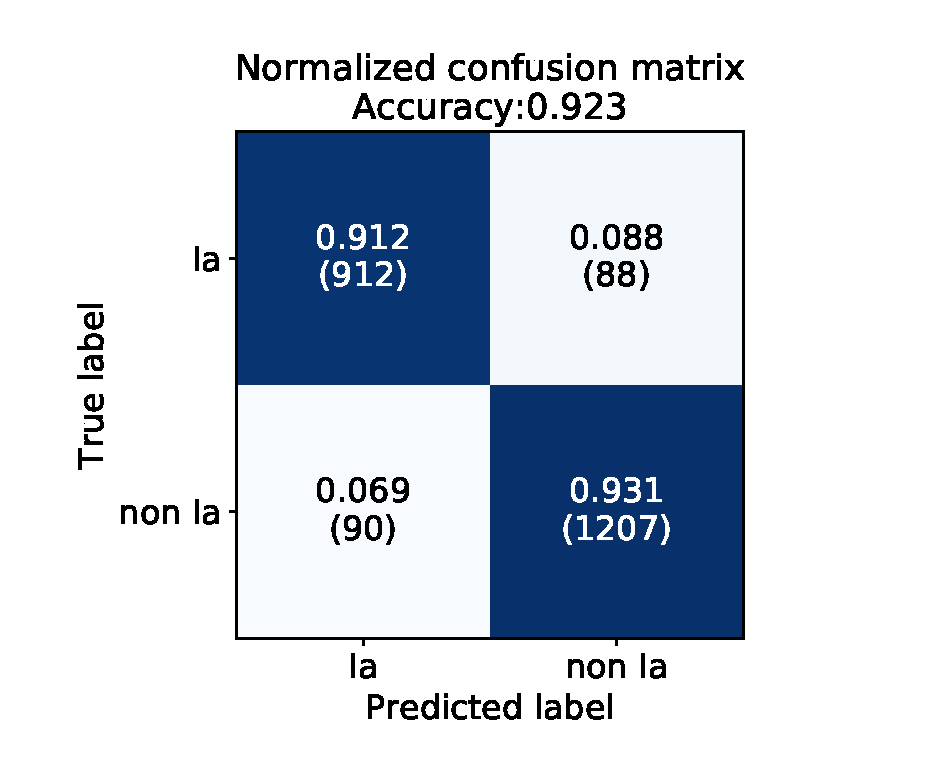
\includegraphics[width=\columnwidth]{figures/07_CM_PLAsTiCC-1st_submission_aug22_2class_2.eps}
            \end{center}
        \end{minipage}
        \begin{minipage}{0.5\hsize}
            \begin{center}
                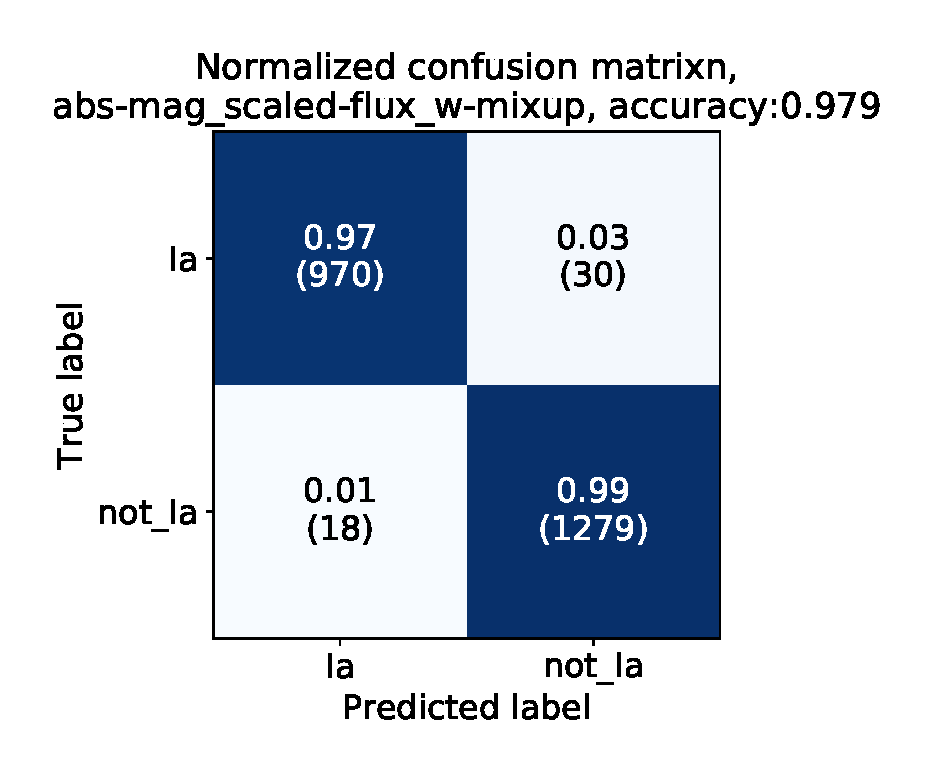
\includegraphics[width=\columnwidth]{figures/03_CM_abs-mag_scaled-flux_w-mixup_predictions_test_2.eps}
            \end{center}
        \end{minipage}
    \end{tabular}  \caption{%
    Normalized confusion matrices of two-class classification results for the PLAsTiCC test set by \citet{boone19a} (left) and our best classifier given pseudo-absolute magnitude and normalized flux (right).
    }%                                                                                           
    \label{fig:comp_plasticc_1st}
\end{figure*}
%
%
%
%
\subsection{Data uncertainty}
%
\DIFdelbegin \DIFdel{The flux error information }\DIFdelend \DIFaddbegin \DIFadd{Information about the flux error }\DIFaddend is also important for the classification of distant SN Ia, which is the main target of the HSC survey\DIFdelbegin \DIFdel{and }\DIFdelend \DIFaddbegin \DIFadd{. In addition, Type SN Ia }\DIFaddend has a small signal-to-noise ratio.
As \DIFdelbegin \DIFdel{shown }\DIFdelend \DIFaddbegin \DIFadd{mentioned }\DIFaddend in section \ref{sec:p}, the signal-to-noise ratio affects the performance of the model.
%
Here, we discuss \DIFdelbegin \DIFdel{how to incorporate }\DIFdelend \DIFaddbegin \DIFadd{the incorporation of }\DIFaddend errors for classification, including \DIFaddbegin \DIFadd{in }\DIFaddend our method.
\citet{charnock17a} \DIFdelbegin \DIFdel{adds }\DIFdelend \DIFaddbegin \DIFadd{added }\DIFaddend the flux error itself as part of the input vector.
In the case of feature-based classification, the flux error is used in \DIFdelbegin \DIFdel{fitting for calculating }\DIFdelend \DIFaddbegin \DIFadd{the fitting process to calculate }\DIFaddend the features, and affects those errors.
The flux error is also used to calculate statistical features such as \DIFdelbegin \DIFdel{'}\DIFdelend \DIFaddbegin \DIFadd{``}\DIFaddend Standard Deviation / Mean\DIFdelbegin \DIFdel{',}\DIFdelend \DIFaddbegin \DIFadd{,'' }\DIFaddend which is one of the features \DIFdelbegin \DIFdel{shown in }\DIFdelend \DIFaddbegin \DIFadd{discussed by }\DIFaddend \citet{narayan18a} and \citet{Muthukrishna_2019}.
\DIFdelbegin \DIFdel{On the other hand, as }\DIFdelend \DIFaddbegin \DIFadd{As }\DIFaddend described in subsection \ref{sec:training}, we calculate the flux error of the simulated training data based on the relationship between the flux and the flux error for each epoch of the observed data.
Then, random numbers that follow a normal distribution defined by the original fluxes and flux errors are input to the classifier as processed fluxes.

The processing of time series data with uncertainty is \DIFdelbegin \DIFdel{an issue }\DIFdelend \DIFaddbegin \DIFadd{problematic }\DIFaddend in many application domains, not only in the \DIFdelbegin \DIFdel{astronomy field }\DIFdelend \DIFaddbegin \DIFadd{field of astronomy}\DIFaddend .
For example, in \DIFaddbegin \DIFadd{the }\DIFaddend similarity matching of time series data with uncertainty,  \DIFdelbegin \DIFdel{it is suggested as a promising method to take into account }\DIFdelend \DIFaddbegin \DIFadd{considering }\DIFaddend continuous correlation in time series such as measuring \DIFaddbegin \DIFadd{the }\DIFaddend distance after filtering by \DIFaddbegin \DIFadd{the }\DIFaddend Uncertain Moving Average (UMA)\citep{Dallachiesa_2012} \DIFaddbegin \DIFadd{is suggested to be a promising approach}\DIFaddend .
UMA filtering uses the correlation of neighboring points and reduces the contribution of observation points with large errors.
We \DIFdelbegin \DIFdel{believe that }\DIFdelend \DIFaddbegin \DIFadd{consider }\DIFaddend the development of a method to efficiently incorporate \DIFdelbegin \DIFdel{such error information is }\DIFdelend \DIFaddbegin \DIFadd{this error information to be }\DIFaddend necessary for improving the classification performance.
%
\subsection{Missing data}
%
Our method \DIFdelbegin \DIFdel{is specialized in }\DIFdelend \DIFaddbegin \DIFadd{was developed specifically for }\DIFaddend the HSC survey, where each observed transient tends to have the same cadence by observing a certain field repeatedly.
However, this method is \DIFdelbegin \DIFdel{not }\DIFdelend \DIFaddbegin \DIFadd{neither }\DIFaddend suitable for processing data with different observation schedules for each object \DIFdelbegin \DIFdel{, or dataset with missing data }\DIFdelend \DIFaddbegin \DIFadd{nor for datasets from which data are missing}\DIFaddend .
In other classification methods, missing data \DIFdelbegin \DIFdel{is }\DIFdelend \DIFaddbegin \DIFadd{are }\DIFaddend interpolated by linear or Gaussian processes \citep{Lochner_2016,Muthukrishna_2019}, or replaced with reference to the flux of adjacent photometric points \citep{charnock17a}.
\DIFdelbegin \DIFdel{We }\DIFdelend \DIFaddbegin \DIFadd{Our approach is to }\DIFaddend handle missing data by preparing multiple classifiers.
The \DIFdelbegin \DIFdel{classifier can }\DIFdelend \DIFaddbegin \DIFadd{advantage of our classifier is that it is able to }\DIFaddend use the photometric information directly \DIFdelbegin \DIFdel{and classify }\DIFdelend \DIFaddbegin \DIFadd{for classification }\DIFaddend with less pre-processing, compared to \DIFdelbegin \DIFdel{the method of interpolation and replacing}\DIFdelend \DIFaddbegin \DIFadd{methods that use interpolation or replacement}\DIFaddend .
In the case of the HSC survey, most of the observation schedules of all supernovae can be roughly divided into two types \DIFdelbegin \DIFdel{, corresponding to }\DIFdelend \DIFaddbegin \DIFadd{that correspond to either the }\DIFaddend Ultra-Deep \DIFdelbegin \DIFdel{and Deep layer}\DIFdelend \DIFaddbegin \DIFadd{or Deep layers}\DIFaddend .
Therefore, \DIFdelbegin \DIFdel{as shown in table \ref{tab:class_flag}, }\DIFdelend we can classify 99.3\% of SNe using only five classifiers with different input \DIFdelbegin \DIFdel{schedule cases}\DIFdelend \DIFaddbegin \DIFadd{schedules}\DIFaddend , including those for SNe data containing missing data \DIFaddbegin \DIFadd{(table \ref{tab:class_flag})}\DIFaddend .
%
%
\subsection{Type fractions of HSC SNe}
The elemental abundance of the solar system \citep{grevesse98a} originates from the cosmic history of SNe \citep{maraston05a,kobayashi00a}.  
Recent studies \DIFdelbegin \DIFdel{show that the solar }\DIFdelend \DIFaddbegin \DIFadd{showed that this elemental }\DIFaddend abundance pattern is observed in other systems \citep{ramirez09a} and clusters \citep{mernier18a}. 
\DIFdelbegin \DIFdel{It is important to investigate }\DIFdelend \DIFaddbegin \DIFadd{Investigation of }\DIFaddend the origin of elements in the context of cosmic evolution \DIFaddbegin \DIFadd{is thus important }\DIFaddend \citep{fukugita04a}. 

It is now well established that \DIFaddbegin \DIFadd{the }\DIFaddend star formation rate \DIFdelbegin \DIFdel{is peaking }\DIFdelend \DIFaddbegin \DIFadd{peaks }\DIFaddend at z$\sim$2, and \DIFaddbegin \DIFadd{that }\DIFaddend the chemical composition of our system \DIFdelbegin \DIFdel{is a mixture of }\DIFdelend \DIFaddbegin \DIFadd{results from both }\DIFaddend SN~Ia and Core-Collapse SNe \citep{tsujimoto95a,kobayashi11a}.
Deriving \DIFdelbegin \DIFdel{SN rate needs a }\DIFdelend \DIFaddbegin \DIFadd{the SN rate would require }\DIFaddend careful analysis \citep{dilday08a,brown19a,frohmaier19a} and \DIFdelbegin \DIFdel{it }\DIFdelend is beyond the scope of this paper, but at least we can \DIFdelbegin \DIFdel{check }\DIFdelend \DIFaddbegin \DIFadd{verify }\DIFaddend the consistency with previous work \DIFdelbegin \DIFdel{on }\DIFdelend \DIFaddbegin \DIFadd{in terms of the }\DIFaddend relative fraction.
\DIFaddbegin \DIFadd{The }\DIFaddend Lick Observatory Supernova Survey \citep{li11a} \DIFdelbegin \DIFdel{reports }\DIFdelend \DIFaddbegin \DIFadd{reported }\DIFaddend the relative ratio \DIFdelbegin \DIFdel{between }\DIFdelend \DIFaddbegin \DIFadd{of }\DIFaddend SN~Ia:Ibc:II to be 0.24:0.19:0.57, \DIFdelbegin \DIFdel{while we have }\DIFdelend \DIFaddbegin \DIFadd{whereas we obtained }\DIFaddend 0.22:0.19:0.59 even at z$\lesssim$0.2. 

Based on our survey depth, we have a complete sampling of SN~Ia up to z$\sim$1.1 \DIFdelbegin \DIFdel{while we lose }\DIFdelend \DIFaddbegin \DIFadd{although we lose the }\DIFaddend completeness of Core-Collapse SN in much lower redshift given the fact that the magnitudes of SN~Ibc and SN~II are fainter by 2$\sim$3 mag at maximum.
\DIFdelbegin \DIFdel{The trend of }\DIFdelend \DIFaddbegin \DIFadd{Increasing redshift causes the }\DIFaddend SN~II fraction \DIFdelbegin \DIFdel{drops while }\DIFdelend \DIFaddbegin \DIFadd{to decrease whereas the }\DIFaddend SN~Ia fraction \DIFdelbegin \DIFdel{rises towards high redshift }\DIFdelend \DIFaddbegin \DIFadd{increases }\DIFaddend as shown in figure \ref{fig:hsc3_type_frac_alongz}. 
\DIFdelbegin \DIFdel{It is simply because of this completeness effect due the the }\DIFdelend \DIFaddbegin \DIFadd{This completeness effect is simply due to the }\DIFaddend magnitude difference and does not reflect the cosmological SN rates.
\DIFdelbegin \DIFdel{If we adopt }\DIFdelend \DIFaddbegin \DIFadd{By adopting }\DIFaddend the SN~Ia rate from \citet{graur14a} and \DIFaddbegin \DIFadd{the }\DIFaddend Core-Collapse SN rate from \citet{strolger15a}, we can estimate the completeness of Core-Collapse SN. 
At z$\sim$0.3\DIFaddbegin \DIFadd{, the }\DIFaddend Core-Collapse SN completeness is 78\%, and it \DIFdelbegin \DIFdel{drops to be }\DIFdelend \DIFaddbegin \DIFadd{is reduced to }\DIFaddend 49\% at z$\sim$0.5. 
The reason \DIFdelbegin \DIFdel{why }\DIFdelend \DIFaddbegin \DIFadd{for the }\DIFaddend SN~II fraction \DIFdelbegin \DIFdel{does not go to }\DIFdelend \DIFaddbegin \DIFadd{not approaching }\DIFaddend zero at z$\sim$1 in \DIFdelbegin \DIFdel{Figure }\DIFdelend \DIFaddbegin \DIFadd{figure }\DIFaddend \ref{fig:hsc3_type_frac_alongz} is that the magnitude \DIFaddbegin \DIFadd{of the }\DIFaddend dispersion of Core-Collapse SN \citep[$\sigma$ $\sim$ 1.2 mag]{li11a,kessler19b} is much larger than that of SN~Ia \citep[$\sigma$ $\sim$ 0.5 mag]{rubin15a}, and they are \DIFdelbegin \DIFdel{factor of 4-5 }\DIFdelend more abundant at z$\sim$1 \DIFdelbegin \DIFdel{\citep{madau98a,hounsell18a}. 
More careful investigation is needed, but we deduce }\DIFdelend \DIFaddbegin \DIFadd{by a factor of 4--5 \citep{madau98a,hounsell18a}. 
Although a more careful investigation would be necessary, we deduce the }\DIFaddend completeness of Core-Collapse SN at z$\sim$1 \DIFdelbegin \DIFdel{is }\DIFdelend \DIFaddbegin \DIFadd{to be }\DIFaddend 12\%.

%
%
%
\section{Conclusions}
%
In this paper, we present a model of a classifier that classifies SN types by directly \DIFdelbegin \DIFdel{inputting photometric data , and its classification performance}\DIFdelend \DIFaddbegin \DIFadd{accepting photometric data as its input. The classification performance of the classifier was discussed in detail}\DIFaddend .
Our DNN classifier is trained with simulated SN photometric data and \DIFdelbegin \DIFdel{classifies }\DIFdelend \DIFaddbegin \DIFadd{was shown to classify }\DIFaddend PLAsTiCC data and actual HSC SNe data with high accuracy of 95.3\% and 84.2\%\DIFdelbegin \DIFdel{respectively.
The study on }\DIFdelend \DIFaddbegin \DIFadd{, respectively.
Our study of }\DIFaddend the number of input dimensions also \DIFdelbegin \DIFdel{shows }\DIFdelend \DIFaddbegin \DIFadd{indicated }\DIFaddend that our classifier can classify the HSC survey data with sufficient accuracy \DIFdelbegin \DIFdel{even for }\DIFdelend \DIFaddbegin \DIFadd{by even using }\DIFaddend two weeks of pre-peak data \DIFdelbegin \DIFdel{from }\DIFdelend \DIFaddbegin \DIFadd{since }\DIFaddend the first detection.
\DIFdelbegin \DIFdel{From these facts, we conclude }\DIFdelend \DIFaddbegin \DIFadd{Based on these results, we concluded }\DIFaddend that this classifier has sufficient classification performance for subsequent type-specific studies and \DIFaddbegin \DIFadd{for the }\DIFaddend selection of follow-up targets even in actual HSC surveys.
%
\begin{ack}
The Hyper Suprime-Cam (HSC) collaboration includes the astronomical communities of Japan, Taiwan, and Princeton University. The HSC instrumentation and software were developed by the National Astronomical Observatory of Japan (NAOJ), the Kavli Institute for the Physics and Mathematics of the Universe (Kavli IPMU), the University of Tokyo, the High Energy Accelerator Research Organization (KEK), the Academia Sinica Institute for Astronomy and Astrophysics in Taiwan (ASIAA), and Princeton University. Funding was contributed by the FIRST program from the Japanese Cabinet Office, the Ministry of Education, Culture, Sports, Science and Technology (MEXT), the Japan Society for the Promotion of Science (JSPS), the Japan Science and Technology Agency (JST), the Toray Science Foundation, NAOJ, Kavli IPMU, KEK, ASIAA, and Princeton University.

\DIFdelbegin \DIFdel{This paper makes }\DIFdelend \DIFaddbegin \DIFadd{The work presented in this paper made }\DIFaddend use of software developed for the Large Synoptic Survey Telescope. We \DIFaddbegin \DIFadd{would like to }\DIFaddend thank the LSST Project for making their code available as free software at http://dm.lsst.org

The Pan-STARRS1 Surveys (PS1) have been made possible through contributions of the Institute for Astronomy, the University of Hawaii, the Pan-STARRS Project Office, the Max-Planck Society and its participating institutes, the Max Planck Institute for Astronomy \DIFdelbegin \DIFdel{, }\DIFdelend \DIFaddbegin \DIFadd{in }\DIFaddend Heidelberg and the Max Planck Institute for Extraterrestrial Physics \DIFdelbegin \DIFdel{, }\DIFdelend \DIFaddbegin \DIFadd{in }\DIFaddend Garching, The Johns Hopkins University, Durham University, the University of Edinburgh, Queen’s University Belfast, the Harvard-Smithsonian Center for Astrophysics, the Las Cumbres Observatory Global Telescope Network Incorporated, the National Central University of Taiwan, the Space Telescope Science Institute, the National Aeronautics and Space Administration under Grant No. NNX08AR22G issued through the Planetary Science Division of the NASA Science Mission Directorate, the National Science Foundation under Grant No. AST-1238877, the University of Maryland, \DIFdelbegin \DIFdel{and }\DIFdelend \DIFaddbegin \DIFadd{the }\DIFaddend Eotvos Lorand University (ELTE)\DIFdelbegin \DIFdel{and the }\DIFdelend \DIFaddbegin \DIFadd{, and }\DIFaddend Los Alamos National Laboratory.

We thank Y. Imoto for his enormous contribution to the development of the classification model, and the data classification.
We also thank T. J. Moriya, J. Jiang\DIFaddbegin \DIFadd{, }\DIFaddend and other members of \DIFaddbegin \DIFadd{the }\DIFaddend HSC transient working group for helpful discussions and comments on the manuscript.

This work is supported by JST CREST Grant Number JPMHCR1414, MEXT KAKENHI Grant Numbers 18H04345 (N.Ya.), 17H06363 (M.T.), and JSPS KAKENHI Grant Numbers 18K03696 (N.S.), 16H02183 (M.T.), 19H00694 (M.T.).

This research is based in part on data collected \DIFdelbegin \DIFdel{at }\DIFdelend \DIFaddbegin \DIFadd{with }\DIFaddend the Subaru Telescope and retrieved from the HSC data archive system, which is operated by the Subaru Telescope and Astronomy Data Center at NAOJ.
\end{ack}
%
%
\appendix 
\section*{Redshift estimation}
\label{sec:est_redshift}
\DIFdelbegin \DIFdel{In }\DIFdelend \DIFaddbegin \DIFadd{The }\DIFaddend HSC-SSP \DIFdelbegin \DIFdel{transient survey, there are }\DIFdelend \DIFaddbegin \DIFadd{Transient Survey includes }\DIFaddend SNe without redshift because their host galaxies are not clearly identified\DIFdelbegin \DIFdel{, called }\DIFdelend \DIFaddbegin \DIFadd{. These SNe are referred to as }\DIFaddend hostless SNe.
In the redshift list of HSC SNe \DIFaddbegin \DIFadd{that was }\DIFaddend used for type classification, 6\% (108/1824) \DIFdelbegin \DIFdel{correspond to them.
To cope with such SNe and }\DIFdelend \DIFaddbegin \DIFadd{corresponds to these hostless SNe.
To be able to process these SNe with our classifier and to address }\DIFaddend the possibility of host galaxy misidentification,
we \DIFdelbegin \DIFdel{can }\DIFdelend \DIFaddbegin \DIFadd{could }\DIFaddend estimate the redshift $z$ of \DIFdelbegin \DIFdel{a }\DIFdelend \DIFaddbegin \DIFadd{an }\DIFaddend SN from the photometric data.

\DIFdelbegin \DIFdel{We use }\DIFdelend \DIFaddbegin \DIFadd{The redshift was estimated by using }\DIFaddend a model with the same structure as \DIFaddbegin \DIFadd{that }\DIFaddend in figure \ref{fig:dnn_model} except that the DNN output is a scalar, and \DIFdelbegin \DIFdel{place no }\DIFdelend \DIFaddbegin \DIFadd{that the model does not include a }\DIFaddend final softmax layer for redshift estimation.
The objective function to optimize is the squared error between the ground truth $z$ and the output value $\hat{y}$.
We \DIFdelbegin \DIFdel{measure }\DIFdelend \DIFaddbegin \DIFadd{measured }\DIFaddend the accuracy of the model with the coefficient of determination $R^2$\DIFdelbegin \DIFdel{, }\DIFdelend \DIFaddbegin \DIFadd{; }\DIFaddend that is,
\begin{eqnarray*}
    R^2 = 1 - \frac{\sum_n \left| z_n - \hat{y}_n \right|^2}{\sum_n \left| z_n - \bar{z} \right|^2}, 
\end{eqnarray*}
where $z_n$ is the redshift value of \DIFaddbegin \DIFadd{the }\DIFaddend $n$-th sample, $\hat{y}_n$ is the output of \DIFaddbegin \DIFadd{the }\DIFaddend $n$-th sample, 
and $\bar{z}$ is the mean redshift of the dataset.
We \DIFdelbegin \DIFdel{perform }\DIFdelend \DIFaddbegin \DIFadd{performed }\DIFaddend the same hyperparameter search in the model as \DIFaddbegin \DIFadd{that described }\DIFaddend in subsection \ref{hyperparametersearch}\DIFdelbegin \DIFdel{including the }\DIFdelend \DIFaddbegin \DIFadd{, 
including }\DIFaddend data augmentation.
The accuracy of this estimator is discussed below.

We \DIFdelbegin \DIFdel{apply }\DIFdelend \DIFaddbegin \DIFadd{applied }\DIFaddend the standard deviation of \DIFaddbegin \DIFadd{the }\DIFaddend normalized residual $(z_{\rm pred}-z_{\rm spec})/(1+z_{\rm spec})$ \citep{Salvato_2009,Salvato_2019}, used in galaxy photo-z estimation, to the performance criteria for redshift estimation.
\DIFdelbegin \DIFdel{In verification }\DIFdelend \DIFaddbegin \DIFadd{Verified }\DIFaddend with Case 0 simulated data, \DIFdelbegin \DIFdel{that }\DIFdelend \DIFaddbegin \DIFadd{the redshifts }\DIFaddend for Ia and \DIFdelbegin \DIFdel{non Ia objects are }\DIFdelend \DIFaddbegin \DIFadd{non-Ia objects were estimated to be }\DIFaddend 0.022 and 0.076, respectively.
For the actual HSC SNe, we used \DIFaddbegin \DIFadd{the }\DIFaddend observationally obtained redshifts of host galaxies (see section \ref{sec:h}) including spec-z and photo-z for comparison with \DIFaddbegin \DIFadd{the }\DIFaddend estimates.
Figure\ \ref{fig:redshift_estimation} shows the comparison between the estimated redshifts and the observed redshifts for \DIFdelbegin \DIFdel{the }\DIFdelend HSC SNe classified as Ia.
The two classes labeled by SALT2 fitting have different distributions, and the events labeled \DIFdelbegin \DIFdel{non Ia }\DIFdelend \DIFaddbegin \DIFadd{non-Ia }\DIFaddend are less accurate in \DIFaddbegin \DIFadd{terms of their }\DIFaddend redshift estimation than Ia.
The normalized residuals for each of \DIFdelbegin \DIFdel{Ia and non Ia }\DIFdelend \DIFaddbegin \DIFadd{the Ia and non-Ia }\DIFaddend Case 0 SNe labeled with SALT2 fitting are normally distributed with standard deviations of 0.066 and 0.138, respectively.
\DIFdelbegin \DIFdel{If the comparison is limited }\DIFdelend \DIFaddbegin \DIFadd{Limiting the comparison }\DIFaddend to SNe in \DIFdelbegin \DIFdel{the }\DIFdelend \DIFaddbegin \DIFadd{a }\DIFaddend host galaxy with spec-z information, \DIFdelbegin \DIFdel{they }\DIFdelend \DIFaddbegin \DIFadd{the standard deviations }\DIFaddend are 0.056 and 0.130\DIFdelbegin \DIFdel{.
Although these }\DIFdelend \DIFaddbegin \DIFadd{, respectively.
Although this }\DIFaddend estimation accuracy is \DIFdelbegin \DIFdel{worse }\DIFdelend \DIFaddbegin \DIFadd{lower }\DIFaddend than the template fitting accuracy using host galaxy photometric data, it is useful not only for hostless SNe, but also to select \DIFaddbegin \DIFadd{the }\DIFaddend host galaxy by comparing the redshift estimated from the SN light curve itself with those of \DIFaddbegin \DIFadd{the }\DIFaddend galaxies.
Furthermore, this distributional difference of residuals leads to the fact that the Ia accuracy can be further improved by excluding events with large residuals \DIFdelbegin \DIFdel{in the estimated }\DIFdelend \DIFaddbegin \DIFadd{when estimating the }\DIFaddend redshift of the SN and host galaxy.
%
\begin{figure*}[htbp]
    \begin{tabular}{cc}
        \begin{minipage}{0.5\hsize}
            \begin{center}
                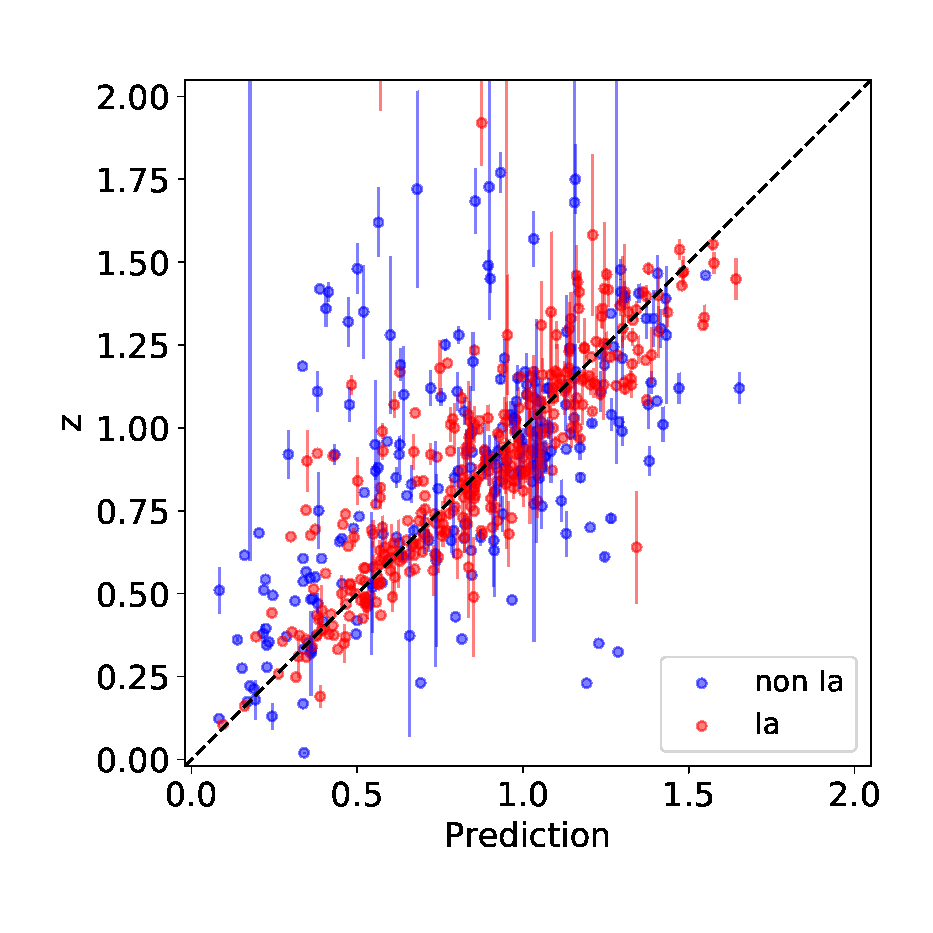
\includegraphics[width=\columnwidth]{figures/redshift_pred_Ia_w_true_label_flagall.eps}
            \end{center}
        \end{minipage}
        \begin{minipage}{0.5\hsize}
            \begin{center}
                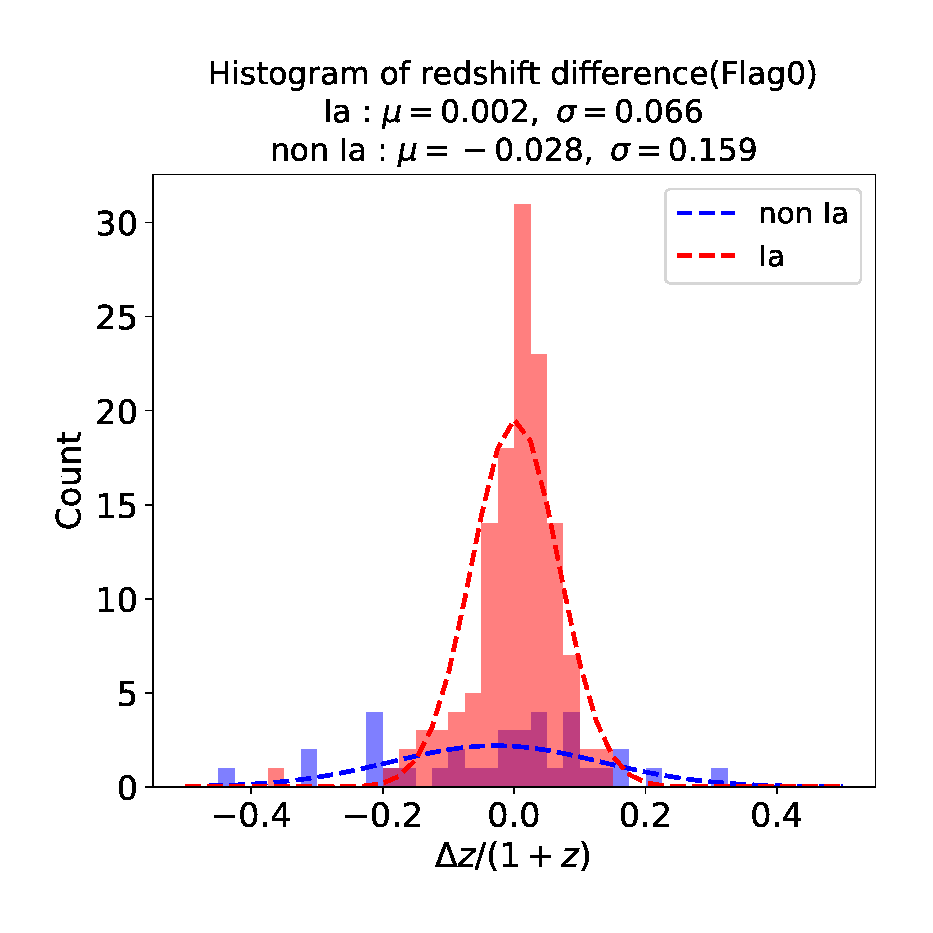
\includegraphics[width=\columnwidth]{figures/redshift_pred_Ia_w_true_label_diff_flag0.eps}
            \end{center}
        \end{minipage}
    \end{tabular}  \caption{%
    (Left) Relation between the machine predictions and the observed redshifts for HSC SNe.
    The dashed line is the line of equality.
    The color difference represents \DIFaddbeginFL \DIFaddFL{the }\DIFaddendFL SALT2 \DIFdelbeginFL \DIFdelFL{fit }\DIFdelendFL \DIFaddbeginFL \DIFaddFL{fitted }\DIFaddendFL label.
    (Right) Normalized residual distribution for Case 0 SNe.
    }%
    \label{fig:redshift_estimation}
\end{figure*}

%
\bibliographystyle{myaasjournal}
\bibliography{hsc,archive}
%


\end{document}

